\documentclass[a4paper,12pt,twoside,BCOR=10mm,numbers=noenddot]{scrbook}

\usepackage[utf8]{inputenc}
\usepackage[T1]{fontenc}
\usepackage[english]{babel}
\babelprovide[import]{icelandic}
\usepackage{mathptmx}
\usepackage{lmodern}
\renewcommand{\rmdefault}{ptm}
\usepackage{microtype}
\usepackage[inner=30mm,outer=25mm,top=25mm,bottom=25mm]{geometry}
\usepackage{graphicx}
\usepackage{booktabs}
\usepackage{tabularx}
\usepackage{array}
\usepackage{colortbl}
\usepackage{float}
\usepackage[format=plain,labelformat=simple,labelsep=colon]{caption}
\usepackage{amsmath}
\usepackage{amssymb}
\usepackage[round,authoryear]{natbib}
\usepackage{url}
\usepackage{xcolor}
\usepackage{tikz}
\usetikzlibrary{positioning}
\usepackage[pdfborder={0 0 0},hidelinks]{hyperref}
\usepackage{scrlayer-scrpage}

\newcolumntype{L}[1]{>{\raggedright\arraybackslash}p{#1}}
\newcommand{\grayhline}{\arrayrulecolor{gray!40}\hline\arrayrulecolor{black}}
\convertcolorspec{RGB}{16,9,159}{rgb}\tmphiblue
\definecolor{hiblue}{rgb}\tmphiblue
\graphicspath{{../main/figures/}}

\setlength{\parskip}{0.5\baselineskip}
\setlength{\parindent}{0pt}
\setlength{\emergencystretch}{2em}
\raggedbottom
\setkomafont{captionlabel}{\normalfont\normalsize\itshape}
\setkomafont{caption}{\normalfont\normalsize\itshape}
\setkomafont{section}{\Large}
\setkomafont{subsection}{\large}
\DeclareTOCStyleEntry[numwidth=3.2em]{tocline}{figure}
\DeclareTOCStyleEntry[numwidth=3.2em]{tocline}{table}
\captionsetup{width=\textwidth,indent=0pt,justification=raggedright,
  singlelinecheck=false,skip=0.5\baselineskip}
% Centre short table captions; keep captions that wrap left-aligned.
\captionsetup[table]{justification=raggedright,singlelinecheck=true}
\clearpairofpagestyles
\ofoot*{\pagemark}
\hypersetup{colorlinks=true,linkcolor=black,citecolor=black,urlcolor=black}
\hypersetup{
  pdftitle={Meteorological Conditions and Rural Injury Accidents in Iceland: Analysis of Accident Frequency and Traffic, 2007--2025},
  pdfauthor={Ásgeir Snær Magnússon},
  pdfsubject={M.Sc. thesis in Software Engineering}
}

\def\thesisyear{2026}
\def\thesismonth{September}
\def\thesisauthor{Ásgeir Snær Magnússon}
\def\thesistitle{Meteorological Conditions and Rural Injury Accidents in Iceland}
\def\thesissubtitle{Analysis of Accident Frequency and Traffic, 2007--2025}
\def\thesisshorttitle{Meteorological Conditions and Rural Injury Accidents}
\def\thesiscredits{30}
\def\thesissubject{Software Engineering}
\def\thesiskind{M.Sc.}
\def\thesiskindformal{Master of Science}
\def\thesisschool{School of Engineering and Natural Sciences}
\def\thesisfaculty{Industrial Engineering, Mechanical Engineering and Computer Science}
\def\thesisaddress{Dunhagi 5}
\def\thesispostalcode{107}
\def\thesistelephone{525 4000}
\def\thesissupervisors{Kristján Jónasson \\ Guðmundur Freyr Úlfarsson}
\def\thesisnrofsupervisors{2}
\def\thesiscommittee{}
\def\thesisexaminer{}
\def\thesisISBN{}
\def\thesisprinting{}
\def\thesislicense{This thesis may not be copied in any form without author permission.}

\newcommand{\removelinebreaks}[1]{%
  \begingroup\def\\{}#1\endgroup}

\begin{document}
\hypersetup{pageanchor=false}
\pagenumbering{Alph}

\begin{titlepage}
  \thispagestyle{empty}
  \begin{tikzpicture}[remember picture,overlay]
    \node[anchor=north west, inner sep=0pt] at (current page.north west)
      {
\includegraphics[width=\paperwidth]{banner}};
    \node(bottom)[shape=rectangle, fill=hiblue, minimum height=10mm,
      minimum width=\paperwidth, anchor=south west] at (current page.south west) {};
    \node[above=0.4cm of bottom] {\sffamily\small
      \textcolor{hiblue}{\textbf{\MakeUppercase{Faculty of \thesisfaculty{}}}}};
  \end{tikzpicture}

  \vspace*{4.1cm}
  \begin{center}
    \huge\sffamily\bfseries \thesistitle{}

    \vspace{0.35cm}
    \normalfont\LARGE\sffamily \thesissubtitle{}

    \vspace{2.5cm}
    \normalfont\Large\sffamily \thesisauthor{}

    \vfill
    \thesismonth{}~\thesisyear{}

    \vspace{0.65cm}
    \normalfont\large\sffamily \thesiskind{}~thesis \\
    in \thesissubject{}

    \vspace{1.45cm}
  \end{center}

  \newpage
  \thispagestyle{empty}\mbox{}

  \newpage
  \thispagestyle{empty}
  \begin{center}
    \vspace*{\stretch{0.5}}
    \Large\sffamily\bfseries \thesistitle{}

    \normalfont\large\sffamily \thesissubtitle{}

    \vspace*{\stretch{1.0}}
    {\sffamily \thesisauthor{}}

    \vspace*{\stretch{1.0}}
    \normalsize \thesiscredits{}~ECTS thesis submitted in partial fulfilment of a \\
    \textit{\thesiskindformal{}} degree in \thesissubject{}

    \vspace*{\stretch{1.0}}
    Supervisors \\
    \thesissupervisors{}

    \vspace*{\stretch{1.0}}
    Faculty of \thesisfaculty{} \\
    \thesisschool{} \\
    University of Iceland \\
    Reykjavík, \thesismonth{}~\thesisyear{}
  \end{center}

  \newpage
  \thispagestyle{empty}
  \vspace*{\fill}
  \sffamily\removelinebreaks{\thesistitle{}} \\
  (\sffamily\thesisshorttitle{}) \\
  \sffamily\removelinebreaks{\thesissubtitle{}} \\

  \thesiscredits{} ECTS thesis submitted in partial fulfilment of a
  \thesiskind{} degree in \thesissubject{} \\

  Faculty of \thesisfaculty{} \\
  \thesisschool{} \\
  University of Iceland \\
  \thesisaddress{} \\
  \thesispostalcode{}, Reykjavík, Iceland \\
  Telephone: \thesistelephone{} \\

  Bibliographic information: \\
  \thesisauthor{} (\thesisyear{}). \emph{\removelinebreaks{\thesistitle{}}},
  \thesiskind{} thesis, Faculty of \thesisfaculty{}, University of Iceland.\\

  Copyright \textcopyright{} \thesisyear{} \thesisauthor{} \\
  \thesislicense{} \\
  Reykjavík, Iceland, \thesismonth{}~\thesisyear{}
\end{titlepage}

\cleardoublepage
\pagenumbering{roman}
\setcounter{page}{5}
\setkomafont{section}{\huge}

\section*{Abstract}
\addcontentsline{toc}{chapter}{Abstract}
This study examines how the occurrence of rural injury accidents varies with
weather conditions in Iceland from 2007--2025. Mean wind speed is the primary
weather measure, with wind gust and temperature as secondary measures.
Accident records were linked to nearby 10-minute weather observations, and
observed accident counts were compared with counts expected from local weather
frequency. Two traffic-based extensions were then applied. The first
approximately reweighted the O/E denominator using traffic responses observed
at daily counters in 2019--2024. The second estimated accident rates per
vehicle-kilometre in a counter-linked sample using observed daily traffic,
rural road length, and pooled monthly weather frequencies. Matched-time and
additional traffic models provided supporting checks.

Of 6,414 rural injury accidents, 6,259 had a qualifying wind observation within
20 km and five minutes of the recorded accident time. At mean wind speeds of at
least 20 m/s, 68 accidents were observed compared with 31.6 expected, giving
O/E 2.15. The approximate traffic correction increased this value to 2.71. In
the separate 694-accident counter-linked analysis, the rate at 20 m/s or above
was 0.667 accidents per million estimated vehicle-kilometres, 5.83 times the
0--5 m/s rate, although only 11 accidents occurred in the upper interval. Wind
gust showed the same general upper-tail pattern, while temperature results were
less consistent across methods.

Overall, rural injury accidents were over-represented during strong wind
relative to local weather frequency. The traffic-based analyses pointed in the
same direction but relied on additional exposure assumptions and smaller
samples. The results describe statistical associations, not causal effects. A
complete national estimate of accident risk per vehicle-kilometre would
require hourly traffic data with broader spatial coverage.
\vfill
\section*{Ágrip}
\addcontentsline{toc}{chapter}{Ágrip}

Í rannsókninni var kannað hvernig umferðarslys með meiðslum í dreifbýli á
Íslandi tengjast veðurskilyrðum á árunum 2007--2025. Megináhersla var á
meðalvindhraða, en vindhviður og hitastig voru einnig skoðuð. Slysagögn voru
tengd við 10 mínútna veðurmælingar frá nálægum veðurstöðvum og skráður fjöldi
slysa borinn saman við væntan fjölda miðað við staðbundna tíðni viðkomandi
veðurskilyrða. Tvær viðbótargreiningar tóku síðan tillit til umferðar. Í þeirri
fyrri var gerð áætluð umferðarleiðrétting á O/E-nefnaranum út frá breytingum í
daglegri umferð á umferðarteljurum 2019--2024. Í þeirri síðari var slysatíðni á hvern ekinn
kílómetra metin í minna úrtaki með daglegum umferðartölum, vegalengd og
mánaðarlegri tíðni veðurs. Pöruð tímagreining og fleiri umferðargreiningar voru
notaðar til stuðnings.

Af 6.414 slysum með meiðslum í dreifbýli var hægt að tengja 6.259 við gilda
vindmælingu innan 20 km og fimm mínútna frá skráðum slysatíma. Við meðalvind
20 m/s eða meiri voru skráð 68 slys, en miðað við staðbundna tíðni slíks
vinds mátti vænta 31,6 slysa. O/E-hlutfallið var því 2,15 og hækkaði í 2,71 eftir áætlaða
umferðarleiðréttingu. Í sérstakri greiningu á 694 slysum með tengingu við
umferðarteljara var áætluð slysatíðni við 20 m/s eða meiri 0,667 slys á hverja
milljón ekinna kílómetra, eða 5,83-föld tíðnin við 0--5 m/s. Aðeins 11 slys voru
í efsta vindbilinu. Sambærilegt mynstur kom fram við miklar vindhviður, en
niðurstöður fyrir hitastig voru breytilegri eftir greiningaraðferð.

Í heild komu slys með meiðslum hlutfallslega oftar fyrir við mikinn vind en
vænta mátti miðað við staðbundna tíðni vindsins. Umferðargreiningarnar bentu í
sömu átt en byggðust á frekari forsendum um umferð og minni úrtökum.
Niðurstöðurnar lýsa tölfræðilegum tengslum en sýna ekki fram á orsakasamband.
Heildstætt mat á slysaáhættu á hvern ekinn kílómetra fyrir landið allt myndi
krefjast umferðargagna á klukkustundargrunni með víðtækari landfræðilegri
þekju.
\newpage
\setkomafont{section}{\Large}
\hypersetup{pageanchor=true}
\tableofcontents
\listoffigures
\listoftables

\chapter*{Abbreviations}
\addcontentsline{toc}{chapter}{Abbreviations}
\begin{tabularx}{\textwidth}{L{0.18\textwidth}X}
ADU & Average annual daily traffic. \\
CI & Confidence interval. \\
O/E & Observed-to-expected accident ratio. \\
OR & Odds ratio. \\
RR & Rate ratio. \\
SDU & Summer daily traffic, June--September. \\
VDU & Winter daily traffic, December--March. \\
VHDU & Spring/autumn daily traffic derived from ADU, SDU and VDU. \\
VKT & Vehicle-kilometres. \\
\end{tabularx}

\cleardoublepage
\pagenumbering{arabic}
\setcounter{page}{1}
\chapter{Introduction}

\section{Context and Motivation}

Weather affects both driving conditions and the decision to travel. Strong
wind can make a vehicle harder to control, low temperature can coincide with
slippery roads, and darkness can reduce visibility. These conditions are
relevant to Icelandic roads, where terrain can produce substantial local
variation in wind \citep{snaebjornsson2007,pu2018}. Precipitation and fog are
also relevant road-weather hazards, but they are context for this study and
are not analysed here.

Previous research provides two reasons to examine wind. Engineering studies
describe mechanisms by which crosswind can destabilise vehicles, while
observational studies compare accident occurrence with the frequency of windy
conditions \citep{baker1986,baker1994risk,edwards1994}. These are complementary
forms of evidence: a physical mechanism does not establish how often accidents
occur across a road network. Reviews also find less consistent road-safety
evidence for wind than for precipitation \citep{theofilatos2014}. Local
evidence is therefore needed to determine whether the same pattern is present
on Icelandic roads.

In Iceland, wind-related road safety has been studied using vehicle-reliability
analyses and operational vehicle-wind models
\citep{snaebjornsson2007,hrafnkelsdottir2020}. This thesis addresses a
different question: whether rural injury accidents are over-represented under
particular weather conditions relative to how often those conditions occur
locally. It then examines how the interpretation changes when available traffic
information is introduced. The study therefore links a long Icelandic accident
series with local weather frequency and two complementary traffic-exposure
approaches, while treating station observations as proxies for road conditions
rather than direct measurements of the forces acting on a vehicle.

The study covers rural injury accidents in Iceland from 2007--2025. Accident
times and locations are linked to nearby 10-minute weather observations. Mean
wind is the primary weather measure; wind gust and temperature are secondary
measures, while season, time of day and daylight provide additional context.

Accident counts alone do not measure accident risk. Severe weather may increase
the hazard faced by each vehicle while also reducing the number of vehicles on
the road. Weather frequency and traffic volume are therefore considered
separately \citep{andrey2003,lord2010,washington2020}.

\section{Aim and Research Questions}

The primary research question is: \emph{How does rural injury-accident
occurrence vary with weather, particularly strong wind, after accounting as
far as possible for local weather frequency and traffic exposure?}

The analysis proceeds in three stages:
\begin{enumerate}
  \item \textbf{Weather-frequency baseline (Q1).} Compare observed accidents
  with the number expected from local weather frequency, by parameter and season.
  This measures over-representation relative to weather time, not risk per vehicle.
  \item \textbf{Approximate traffic correction (Q2).} Establish how traffic
  changes with weather, then use the observed counter response to reweight the
  baseline comparison. This asks whether lower traffic explains the wind pattern.
  \item \textbf{Counter-based accident rates (Q3).} Relate accident counts to
  estimated vehicle-kilometres using daily traffic, rural road length and monthly
  weather frequencies. Compare with allocation using the actual day's weather.
\end{enumerate}

Q1--Q3 identify analysis stages addressing this question, not repeated estimates
of one parameter. The baseline and approximate correction cover 2007--2025;
the rate analysis uses a smaller counter-linked sample from 2019--2024.
Matched-time and older traffic models provide secondary robustness checks.
Minor injury and serious or fatal injury form disjoint components of all injury.
The study estimates associations, not causal effects or a complete national
accident rate per vehicle-kilometre.

\section{Thesis Outline}

Chapter 2 gives the background for the weather and traffic comparisons.
Chapter 3 describes the data, data preparation, and statistical methods.
Chapter 4 presents the three main analyses in research-question order, followed
by supporting checks. Chapter 5 discusses their interpretation and limitations,
and Chapter 6 gives the conclusions. The appendix contains additional checks
that support interpretation of the main results.

\chapter{Background}

\section{Wind and Rural Road Accidents}

Crosswind can produce overturning, lateral sideslip, or excessive yaw. The
critical condition depends on vehicle geometry and mass, vehicle speed, road
friction, wind direction, and driver response rather than wind speed alone
\citep{baker1986,baker1994risk}. High-sided vehicles are particularly exposed,
but the physical mechanisms also provide a reason to examine loss-of-control
accidents more generally. These engineering studies establish physical
plausibility and vehicle-specific failure mechanisms; they do not by
themselves establish a population-level association between wind and accident
occurrence.

This problem is directly relevant in Iceland, where terrain can accelerate and
redirect near-surface wind over short distances. An Icelandic reliability
study by \citet{snaebjornsson2007} modelled accident probability as a combined
function of wind velocity and direction, road camber and friction, and vehicle
speed.
A station measures wind at one point, whereas vehicle stability also depends
on the wind's direction relative to the road and on local road conditions.
Terrain between a station and a road can alter the wind reaching the vehicle.
Station observations therefore remain exposure proxies, and a shorter
matching distance does not guarantee identical conditions. Mobile road
measurement research similarly shows that roadside terrain creates marked
spatial variation that a sparse fixed-station network cannot fully resolve
\citep{pu2018}.

Vegagerðin has developed a vehicle-wind model to support decisions about
hazardous conditions and road closures, while also noting the limited
experimental evidence available for passenger cars \citep{hrafnkelsdottir2020}. The present thesis does not test that
operational model; it examines population-level accident occurrence using a
separate data design.

Empirical work has compared the share of accidents occurring in high wind with
the share of time that high wind was observed, an approach closely related to
the observed/expected comparison used here \citep{edwards1994}. Studies linking
crashes to nearby weather stations likewise show that station observations can
be informative while retaining measurement error \citep{young2007}. More broadly,
\citet{theofilatos2014} report less consistent road-safety evidence for wind
than for precipitation.

\section{Temperature, Daylight, and Time of Day}

Temperature, daylight, and time of day add context that wind alone cannot
provide. They affect road-surface conditions, visibility, travel patterns, and
the composition of road users, but accident counts in these categories are not
rates unless the corresponding amount of travel is known. Temperature effects
can also be non-linear and season-specific: a Seoul time-series study found its
strongest cold-weather association below freezing in winter, while an hourly
case-crossover study in Shenzhen found a J-shaped temperature relationship
\citep{lee2014,zhan2020}. Temperature is therefore compared with its local
seasonal frequency rather than treated as having one linear effect.

Darkness presents the same denominator problem. A method developed using
Norwegian, Swedish, and Dutch data compared daylight and darkness within clock
time and season, avoiding the interpretation of raw night-time counts as risk
\citep{johansson2009}. Here, raw hour, season, and daylight counts describe the
sample. Matched daylight and adjusted severity models are used for numerical
comparisons.

\section{Traffic and Accident Rates}

Weather can change the amount of traffic as well as the hazard. Research using
automatic traffic recorders shows that extreme weather variables, including
wind, can reduce or redistribute hourly traffic volume
\citep{sathiaraj2018}. Accident counts during strong wind can remain low even if
risk to each travelling vehicle is higher. High-resolution crash studies
illustrate the value of hourly weather data rather than daily or monthly
averages \citep{xing2019}. The analyses distinguish
three quantities: accident occurrence relative to weather frequency,
rates based on estimated vehicle-kilometres, and changes in observed daily
traffic. Studies with real-time traffic, weather, and road geometry show what
a more complete analysis could achieve when such data are available
\citep{ahmed2012}.

\chapter{Data and Methods}

\section{Data}

\subsection{Source Data}

Table~\ref{tab:sources} summarises the source datasets. Official documentation
for each source is listed in the bibliography
\citep{samgongustofaAccidents,vedurApi,vegagerdinTraffic,hagstofaThettbyli}.

\begin{table}[H]
\centering
\small
\renewcommand{\arraystretch}{1.12}
\caption{Source datasets. The study period is 2007--2025.}
\label{tab:sources}
\begin{tabularx}{\textwidth}{L{0.09\textwidth}L{0.22\textwidth}L{0.33\textwidth}L{0.25\textwidth}}
\toprule
Data & Provider & Contents & Coverage \\
\midrule
Accident & Samgöngustofa &
Accident events and road links &
126,607 events and 126,610 road links, 2007--2025 \\
Weather & Icelandic Meteorological Office (IMO) &
10-minute weather observations and station metadata &
232,459,562 observations from 338 stations; 438 station records, 2007--2025 \\
Traffic and roads & Vegagerðin &
Annual road traffic, daily counter reports, counter locations, and road geometry &
33,757 section-years, 2000--2025; 1,033,659 counter channel-days, 2019--2024 \\
Urban areas & Statistics Iceland & Urban-area polygons &
97 polygons in the 2020--2024 release \\
\bottomrule
\end{tabularx}
\end{table}

Records from the year 2025 are included in the accident, injury, vehicle,
road-link, annual-traffic and weather datasets under the same selection and
quality criteria as records from earlier years. Daily counter data are
available through 2024. Table~\ref{tab:definitions} defines the weather and
traffic quantities used in the subsequent comparisons.

\begin{table}[H]
\centering
\small
\caption{Definitions used throughout the thesis.}
\label{tab:definitions}
\begin{tabularx}{\textwidth}{L{0.12\textwidth}L{0.34\textwidth}X}
\toprule
Term & Definition & Use in this thesis \\
\midrule
\texttt{f} & 10-minute mean wind speed, m/s & Main weather measure, matched within five minutes of the accident time. \\ \grayhline
\texttt{fg} & Wind gust reported in the same 10-minute observation, m/s & Additional weather measure; not a daily maximum. \\ \grayhline
\texttt{t} & Air temperature reported with each 10-minute observation, \(^{\circ}\)C & Additional weather measure matched independently. \\ \grayhline
O/E & Observed accidents divided by accidents expected from local weather frequency & Main relative-occurrence result; traffic is not included. \\ \grayhline
ADU & Average vehicles per day over the year & Used to check and derive annual traffic quantities. \\ \grayhline
SDU & Average vehicles per day in June--September & Official summer traffic value. \\ \grayhline
VDU & Average vehicles per day in December--March & Official winter traffic value. \\ \grayhline
VHDU & Average vehicles per day in April--May and October--November &
Spring/autumn daily traffic calculated as the residual from ADU, SDU and VDU. \\
\bottomrule
\end{tabularx}
\end{table}

\subsection{Accident Data}

The accident dataset contains 126,607 records from 2007--2025
\citep{samgongustofaAccidents}. One record lacks valid temporal or spatial
information, leaving 126,606 valid records.

Rural status is derived from accident coordinates and Statistics Iceland
urban-locality polygons \citep{hagstofaThettbyli}. Points inside an urban polygon
are classified as Urban, and valid points outside all polygons as Rural. A
defined Vestmannaeyjar area is also classified as Urban. The same 2020--2024
polygon dataset is applied to the full 2007--2025 accident period. Changes in
urban boundaries before 2020 are not represented.

Applying this rural classification yields 24,005 accidents, of which 6,414
involve injury. Of these, 6,259 have a qualifying primary weather match
within 20 km and five minutes.

Accident severity is recorded in \texttt{meidsli}: code 1 denotes a fatal
accident, code 2 a serious accident, code 3 a minor-injury accident, and code 4
an accident without injury. The main outcome is
\(\texttt{meidsli}\leq3\). The serious or fatal comparison uses
\(\texttt{meidsli}\leq2\). The source data also contain 17,591 rural
damage-only accidents; these are outside the injury outcome.

For the reader-facing results, injury accidents are divided into two disjoint
groups: minor injury (\texttt{meidsli}=3) and serious or fatal injury
(\texttt{meidsli}=1 or 2). The O/E calculation for these groups is described
in Section~\ref{sec:weather-frequency}.

Table~\ref{tab:cleaned-accident-example} illustrates the cleaned accident
record before weather matching. Date, time, road location, rural classification,
injury category and vehicle count describe the event; weather measurements are
added in a later linkage step. The example is a single-vehicle minor-injury
accident and is not intended to represent the frequency of accident types.

\begin{table}[H]
\centering
\small
\caption[Example of a cleaned rural injury accident record.]{Example of a cleaned rural injury accident record. The table illustrates accident-level information retained before weather matching. The source identifier alone is masked; time and coordinates are reproduced as recorded.}
\label{tab:cleaned-accident-example}
\begin{tabular}{ll}
\toprule
Field & Example value \\
\midrule
Example identifier & A (source identifier omitted) \\ \grayhline
Date & 2007-01-03 \\ \grayhline
Recorded time & 18:08:00 \\ \grayhline
Registered road section & 1-g8 \\ \grayhline
Latitude / longitude (degrees) & 64.57709888007743, -21.879289941375845 \\ \grayhline
Area classification & Rural \\ \grayhline
Injury category & Minor injury \\ \grayhline
Involved vehicles & 1 \\
\bottomrule
\end{tabular}
\end{table}


Figure~\ref{fig:accident-map} shows the geographic distribution of the rural
injury sample and highlights accidents matched to strong mean wind.

\begin{figure}[htbp]
\centering
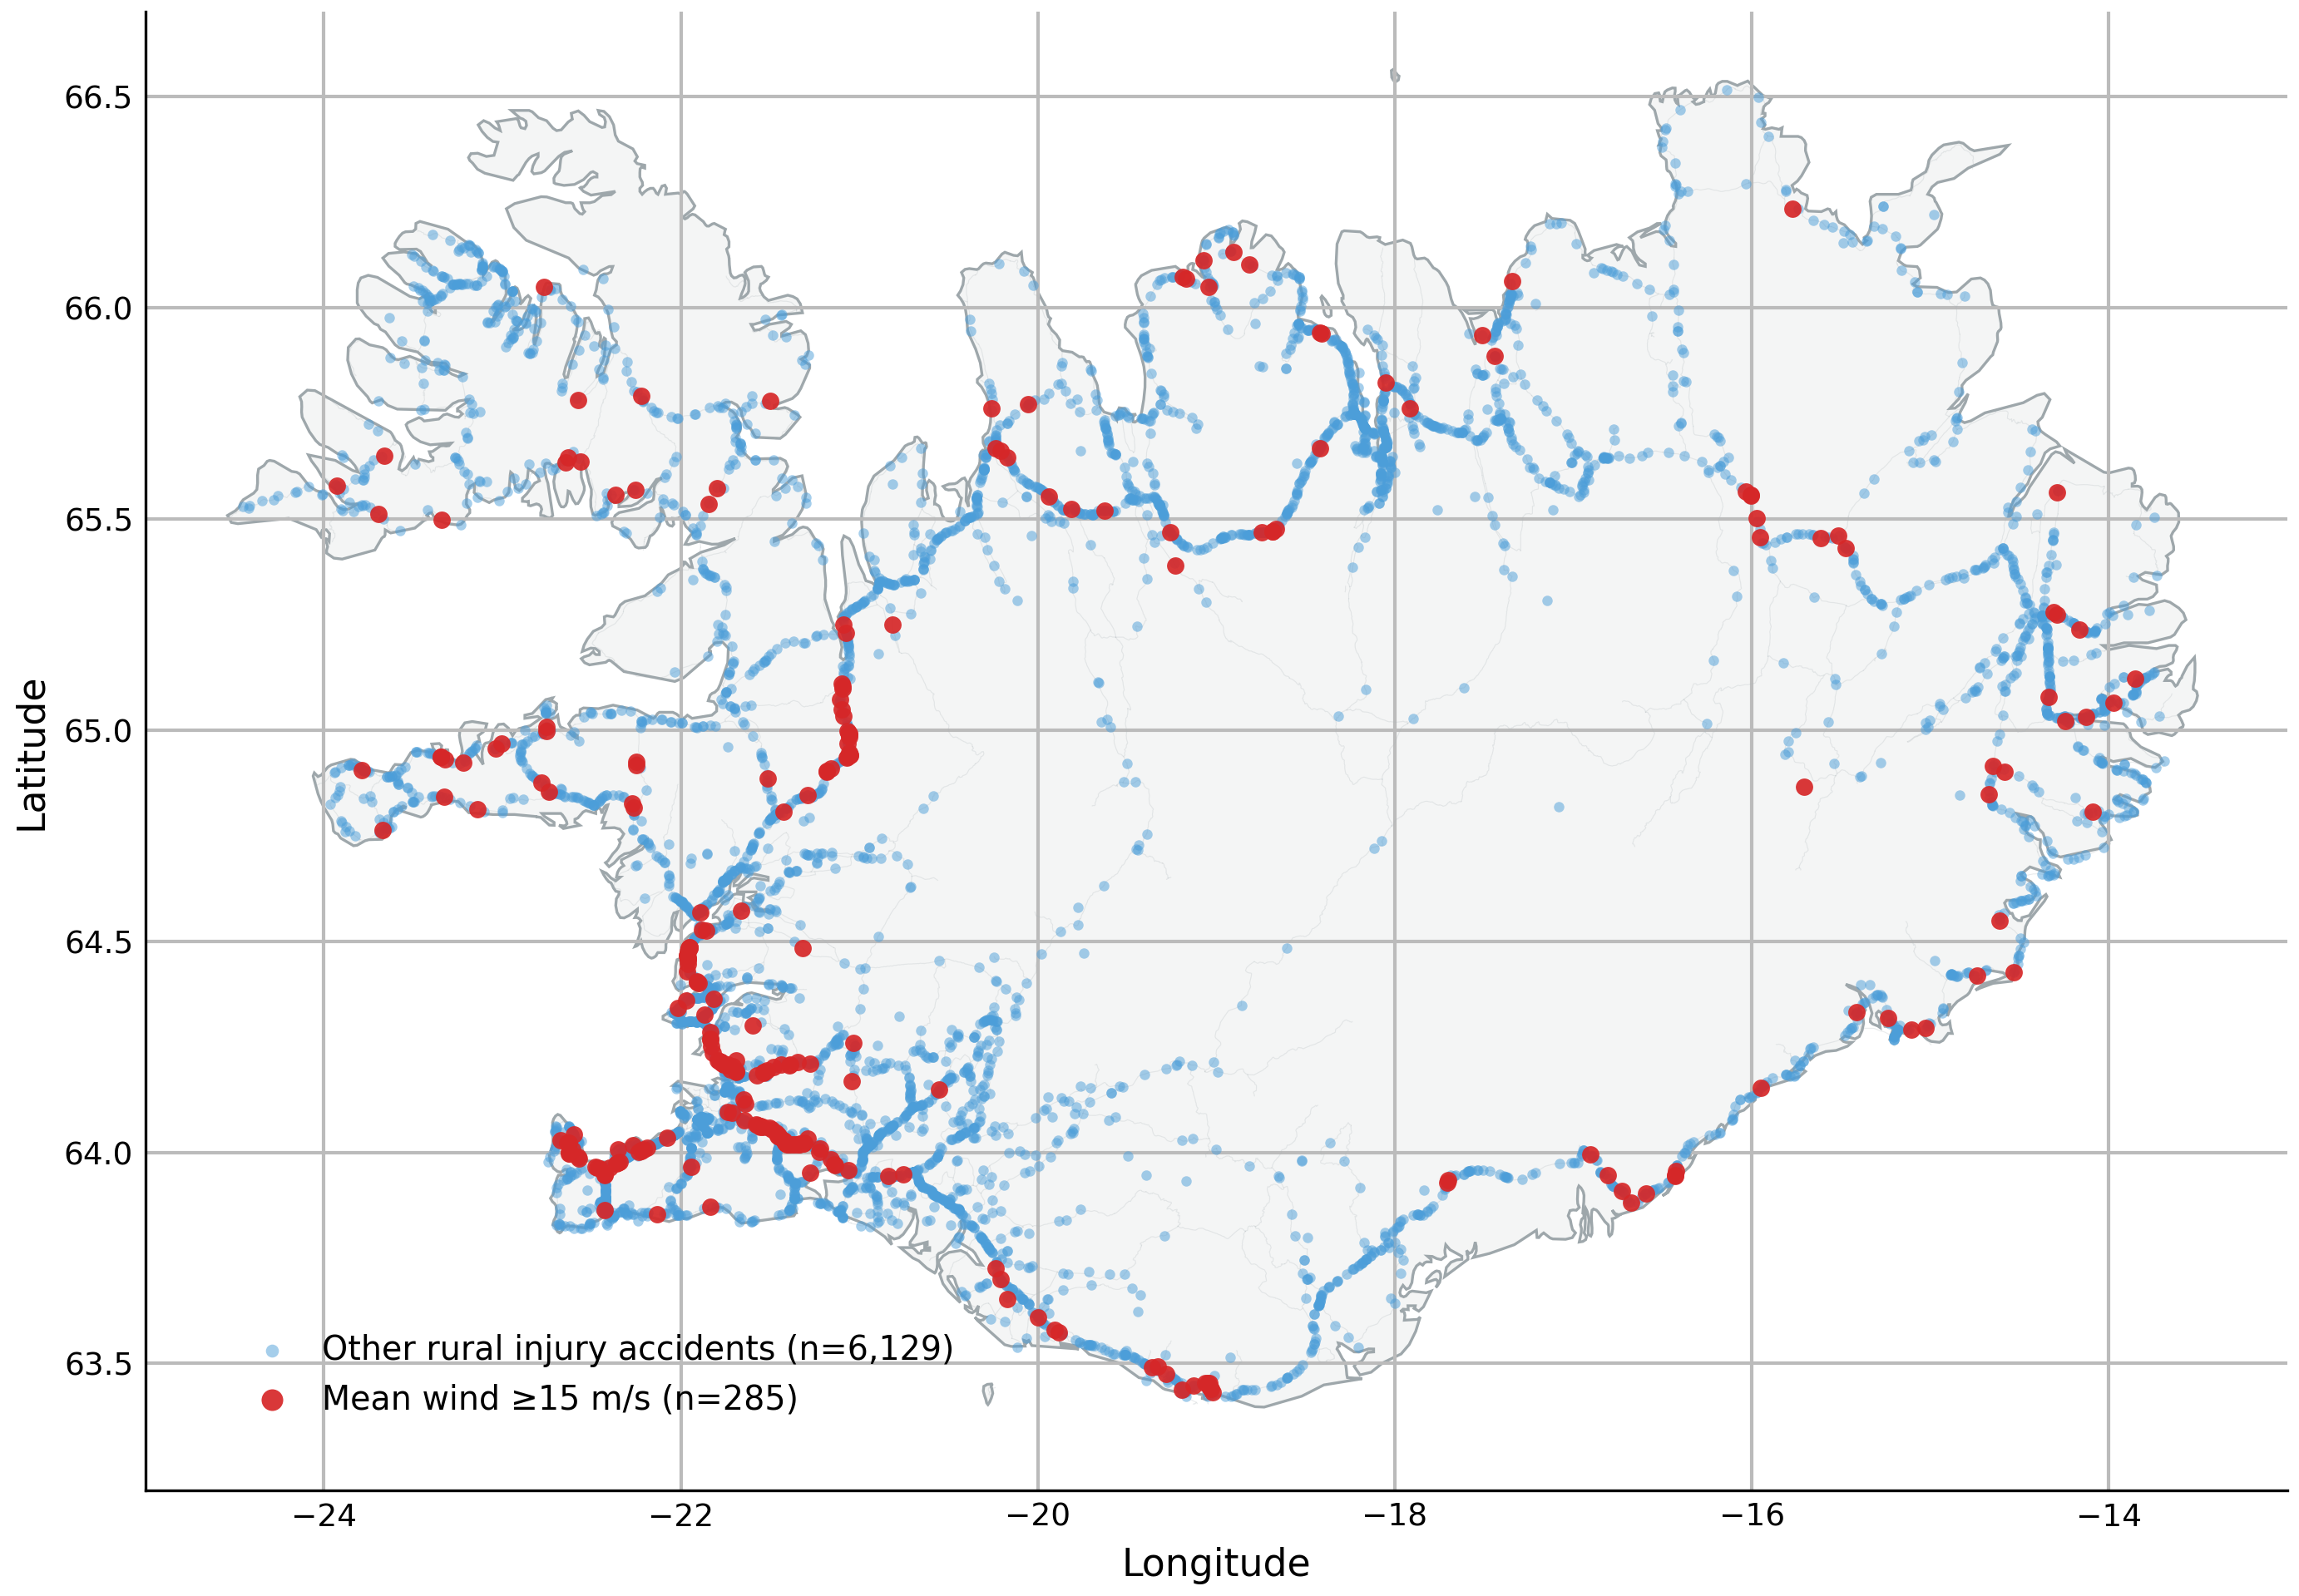
\includegraphics[width=0.96\textwidth]{accident_map.png}
\caption[Locations of rural injury accidents and strong-wind matches.]{Locations of the 6,414 rural injury accidents. Accidents matched to
mean wind of at least 15 m/s are highlighted. The map shows the spatial
coverage of the study and is not a regional accident-rate map.}
\label{fig:accident-map}
\end{figure}

\subsection{Weather Data}

The weather dataset contains 10-minute observations from Icelandic weather
stations. The variables used here are 10-minute mean wind speed (\texttt{f}), reported
wind gust (\texttt{fg}), and temperature (\texttt{t}). For each accident, the
gust is taken from the same matched 10-minute observation as mean wind; it is
not the maximum across the accident day. Mean wind speed remains the main
weather measure. A wind observation is used when

\[
0 \leq f < 45, \qquad 0 \leq fg < 65, \qquad fg + 0.5 \geq f.
\]

Rows missing either \texttt{f} or \texttt{fg} are excluded. Negative values,
values at or above either upper limit, and
internally inconsistent values where \texttt{fg = 0} but \texttt{f > 0} are
excluded. These quality exclusions are summarised in
Table~\ref{tab:weather-cleaning}. A value of \texttt{f = 0} alone is
kept. Only uninterrupted all-zero runs where \texttt{f = fg = 0} for at
least two hours are excluded as potentially frozen sensors. Missing temperature
does not affect whether a wind observation is used.

Each accident is matched to the geographically nearest station with a
quality-controlled wind observation at one of the two adjacent timestamps on
the 10-minute observation grid. The selected observation is therefore no more
than five minutes from the recorded accident time. Because matching is based on
absolute time difference, the adjacent observation can fall on the neighbouring
calendar day for accidents occurring within five minutes of midnight. The
maximum matching distance is 20 km. The matching dataset includes all 6,414
accidents and records whether each accident meets the weather-match criterion.

Temperature is matched independently within the same 20 km and five-minute
limits. The nearest valid value between $-30$ and
$30\,^{\circ}\mathrm{C}$ may therefore come from a different station when the
wind station lacks temperature. In the final analysis dataset, however, all
6,259 wind and temperature matches use the same station and observation time.

The IMO supplied observations of time, station, temperature, mean wind, and
gust. The same quality-controlled weather data are used for accident matching,
background frequencies, matched control times, and traffic analyses. No
temperature value is imputed.

Table~\ref{tab:match-quality} reports spatial and temporal match quality for
wind and temperature. Table~\ref{tab:weather-cleaning} then summarises the
wind-quality exclusions and retained observations.

\begin{table}[H]
\centering
\footnotesize
\caption[Weather-match coverage and distance.]{Share of accidents with weather information from a station with a valid measurement within 20 km. Distance is shown as median / 90th percentile; every retained observation is within five minutes of the accident time.}
\label{tab:match-quality}
\begin{tabular}{lrrrr}
\toprule
Variable & Accidents & Share & Stations & Distance (km) \\
\midrule
Mean wind and gust & 6,259 & 97.6\% & 279 & 5.1 / 12.3 \\ \grayhline
Temperature & 6,259 & 97.6\% & 279 & 5.1 / 12.3 \\
\bottomrule
\end{tabular}
\end{table}


\begin{table}[htbp]
\centering
\small
\caption[Overview of cleaning of wind measurement records, 2007--2025.]{Overview of cleaning of wind measurement records, 2007--2025. Cleaning-rule shares use all supplied observations. Every supplied station-year contains at least one wind measurement.}
\label{tab:weather-cleaning}
\begin{tabular}{lrr}
\toprule
Category & Records & Share \\
\midrule
All supplied station-time observations & 232,459,562 & 100.00\% \\ \grayhline
Missing \texttt{f} or \texttt{fg} & 261,519 & 0.11\% \\ \grayhline
$f<0$, $fg<0$, $f\geq45$ or $fg\geq65$ m/s & 8,766 & 0.00\% \\ \grayhline
$fg=0<f$ or $fg+0.5<f$ (m/s) & 257,245 & 0.11\% \\ \grayhline
All-zero runs $\geq 2$ hr & 1,473,082 & 0.63\% \\ \midrule
Wind observations retained & 230,458,950 & 99.14\% \\
\bottomrule
\end{tabular}
\end{table}


The wind-quality rules exclude 2,000,612 observations and retain 230,458,950
(99.14\%). The largest excluded category is uninterrupted all-zero runs, which
is reported separately because it reflects the rule for possible instrument
stoppages rather than a missing observation. The audit reports each rule
separately and uses all supplied weather observations from 2007--2025. For each
accident's station and season, the O/E expected count uses all quality-controlled
background observations in that station--season group, not only observations
recorded on accident days.



\subsection{Traffic Data}

Daily counter data underpin Q2 and Q3, while annual road-section traffic is
used in supporting analyses.

Annual road-section data provide average annual daily traffic (ADU), summer
daily traffic (SDU), winter daily traffic (VDU), section length, and annual
vehicle-kilometres for 2000--2025 \citep{vegagerdinTraffic}. The road-section
comparison uses the years shared with the accident study, 2007--2025.
Following the official definitions, SDU
covers June--September and VDU covers December--March. These data can be linked
to accidents with a registered road-section identifier, but this linkage is
considerably more restrictive than the weather matching. Table~\ref{tab:traffic-periods} distinguishes
the published averages from the derived spring/autumn value.

\begin{table}[H]
\centering
\small
\caption{Official traffic averages and the spring/autumn daily traffic value
used in the annual-traffic analysis.}
\label{tab:traffic-periods}
\begin{tabularx}{\textwidth}{L{0.27\textwidth}L{0.25\textwidth}X}
\toprule
Period & Months & Daily traffic reference \\
\midrule
ADU (\emph{\'arsdagsumfer\dh}) & Full calendar year & Official annual daily traffic \\
VDU (\emph{vetrardagsumfer\dh}) & December--March & Official winter daily traffic \\
SDU (\emph{sumardagsumfer\dh}) & June--September & Official summer daily traffic \\
VHDU (vor- og haustdagsumferð) &
April--May and October--November &
Residual daily average calculated from ADU, SDU, VDU, and the number of days in each period \\
\bottomrule
\end{tabularx}
\end{table}

Throughout the analyses, the four study seasons are aligned with these
traffic periods: winter is December--March, spring is April--May, summer is
June--September, and autumn is October--November. These are study-specific
traffic-aligned seasons rather than conventional three-month meteorological
seasons. Using June--September as summer keeps the weather comparison aligned
with the Icelandic road authority's summer traffic period; it is an operational
definition, not a claim that weather is uniform across those months. The IMO
also uses June--September when summarising the Icelandic summer
\citep{vedurSummer2025}.
VHDU is not calculated as \(ADU-SDU-VDU\). Annual traffic implied by
ADU is first converted to a calendar-year total; the day-weighted SDU and VDU
totals are subtracted, and the remainder is divided by the number of spring and
autumn days:
\[
VHDU=\frac{D_{year}ADU-D_{VDU}VDU-D_{SDU}SDU}{D_{VHDU}}.
\]
Here, each \(D\) is the number of calendar days in that period. VHDU is
therefore a residual estimate rather than an additional official traffic
measure.

Daily traffic counts extracted from Vegagerðin reports cover 2019--2024 and
provide observed totals at selected counter sites. They underpin the traffic
response used in Q2 and the counter-linked exposure calculation in Q3, but do
not provide hourly traffic at accident locations. More than one counter may occur on a road section, and counter
positions are estimated from the registered road geometry. These data remain
separate from the primary O/E calculation.

Of 68,946 annual road-section--year--period records, 61,442 have nearby usable
wind data; separately, 763,171 of 774,274 daily counter-days have a matched
daytime wind summary. The smaller linked accident samples used by the
traffic models are reported in Chapter 4.

\subsection{Selection Summary}

Table~\ref{tab:data-trimming} summarises the main data reductions. Selection
for the study area and injury outcome is distinguished from invalid or missing
measurements: an excluded record is not necessarily an erroneous record. The
traffic-based rate analysis starts with the 1,863 rural injury accidents in
2019--2024; the broader weather and annual-traffic samples cover 2007--2025.
Traffic-period rows and counter-days are exposure records rather than accident
counts, so the rows in the table are separate selections rather than one
successive filtering chain.

\begin{table}[H]
\centering
\footnotesize
\caption[Primary data selections.]{Overview of primary data selections for accidents, weather and traffic counts. The first four rows are sequential; the last three rows start from separate populations. Each removal percentage uses the count entering that row.}
\label{tab:data-trimming}
\begin{tabularx}{\textwidth}{L{0.23\textwidth}rL{0.13\textwidth}rX}
\toprule
Selection & Entering & Removed at step (\%) & Retained & Reason \\
\midrule
Valid accident records & 126,607 & $<0.01$\% & 126,606 & Invalid time or coordinates. \\ \grayhline
Rural accidents & 126,606 & 81.04\% & 24,005 & Inside the urban study boundary. \\ \grayhline
Rural injury accidents & 24,005 & 73.28\% & 6,414 & No recorded injury. \\ \grayhline
Accidents for weather-only analysis & 6,414 & 2.42\% & 6,259 & No qualifying weather within 20 km and five minutes. \\ \grayhline
Accidents for VKT analysis & 1,863 & 62.75\% & 694 & Separate 2019--2024 sample: counter linkage, daytime, weather and traffic eligibility. \\ \grayhline
Wind observations & 232,459,562 & 0.86\% & 230,458,950 & Wind exclusions in the cleaning overview. \\ \grayhline
Counter-days for traffic-response analysis & 774,274 & 1.43\% & 763,171 & Usable daytime weather summary. \\
\bottomrule
\end{tabularx}
\end{table}


\subsection{Descriptive Accident Patterns}

Figure~\ref{fig:accident-conditions} shows when the selected accidents occurred
and the conditions recorded with them. The blue and red groups are the same
separate severity groups used in the O/E figures. These are raw counts:
more accidents in an hour or season may reflect more traffic, and the panels
do not estimate accident risk. Vehicle counts and accident-type composition
are shown in Appendix~\ref{app:accident-characteristics}.

\begin{figure}[htbp]
\centering
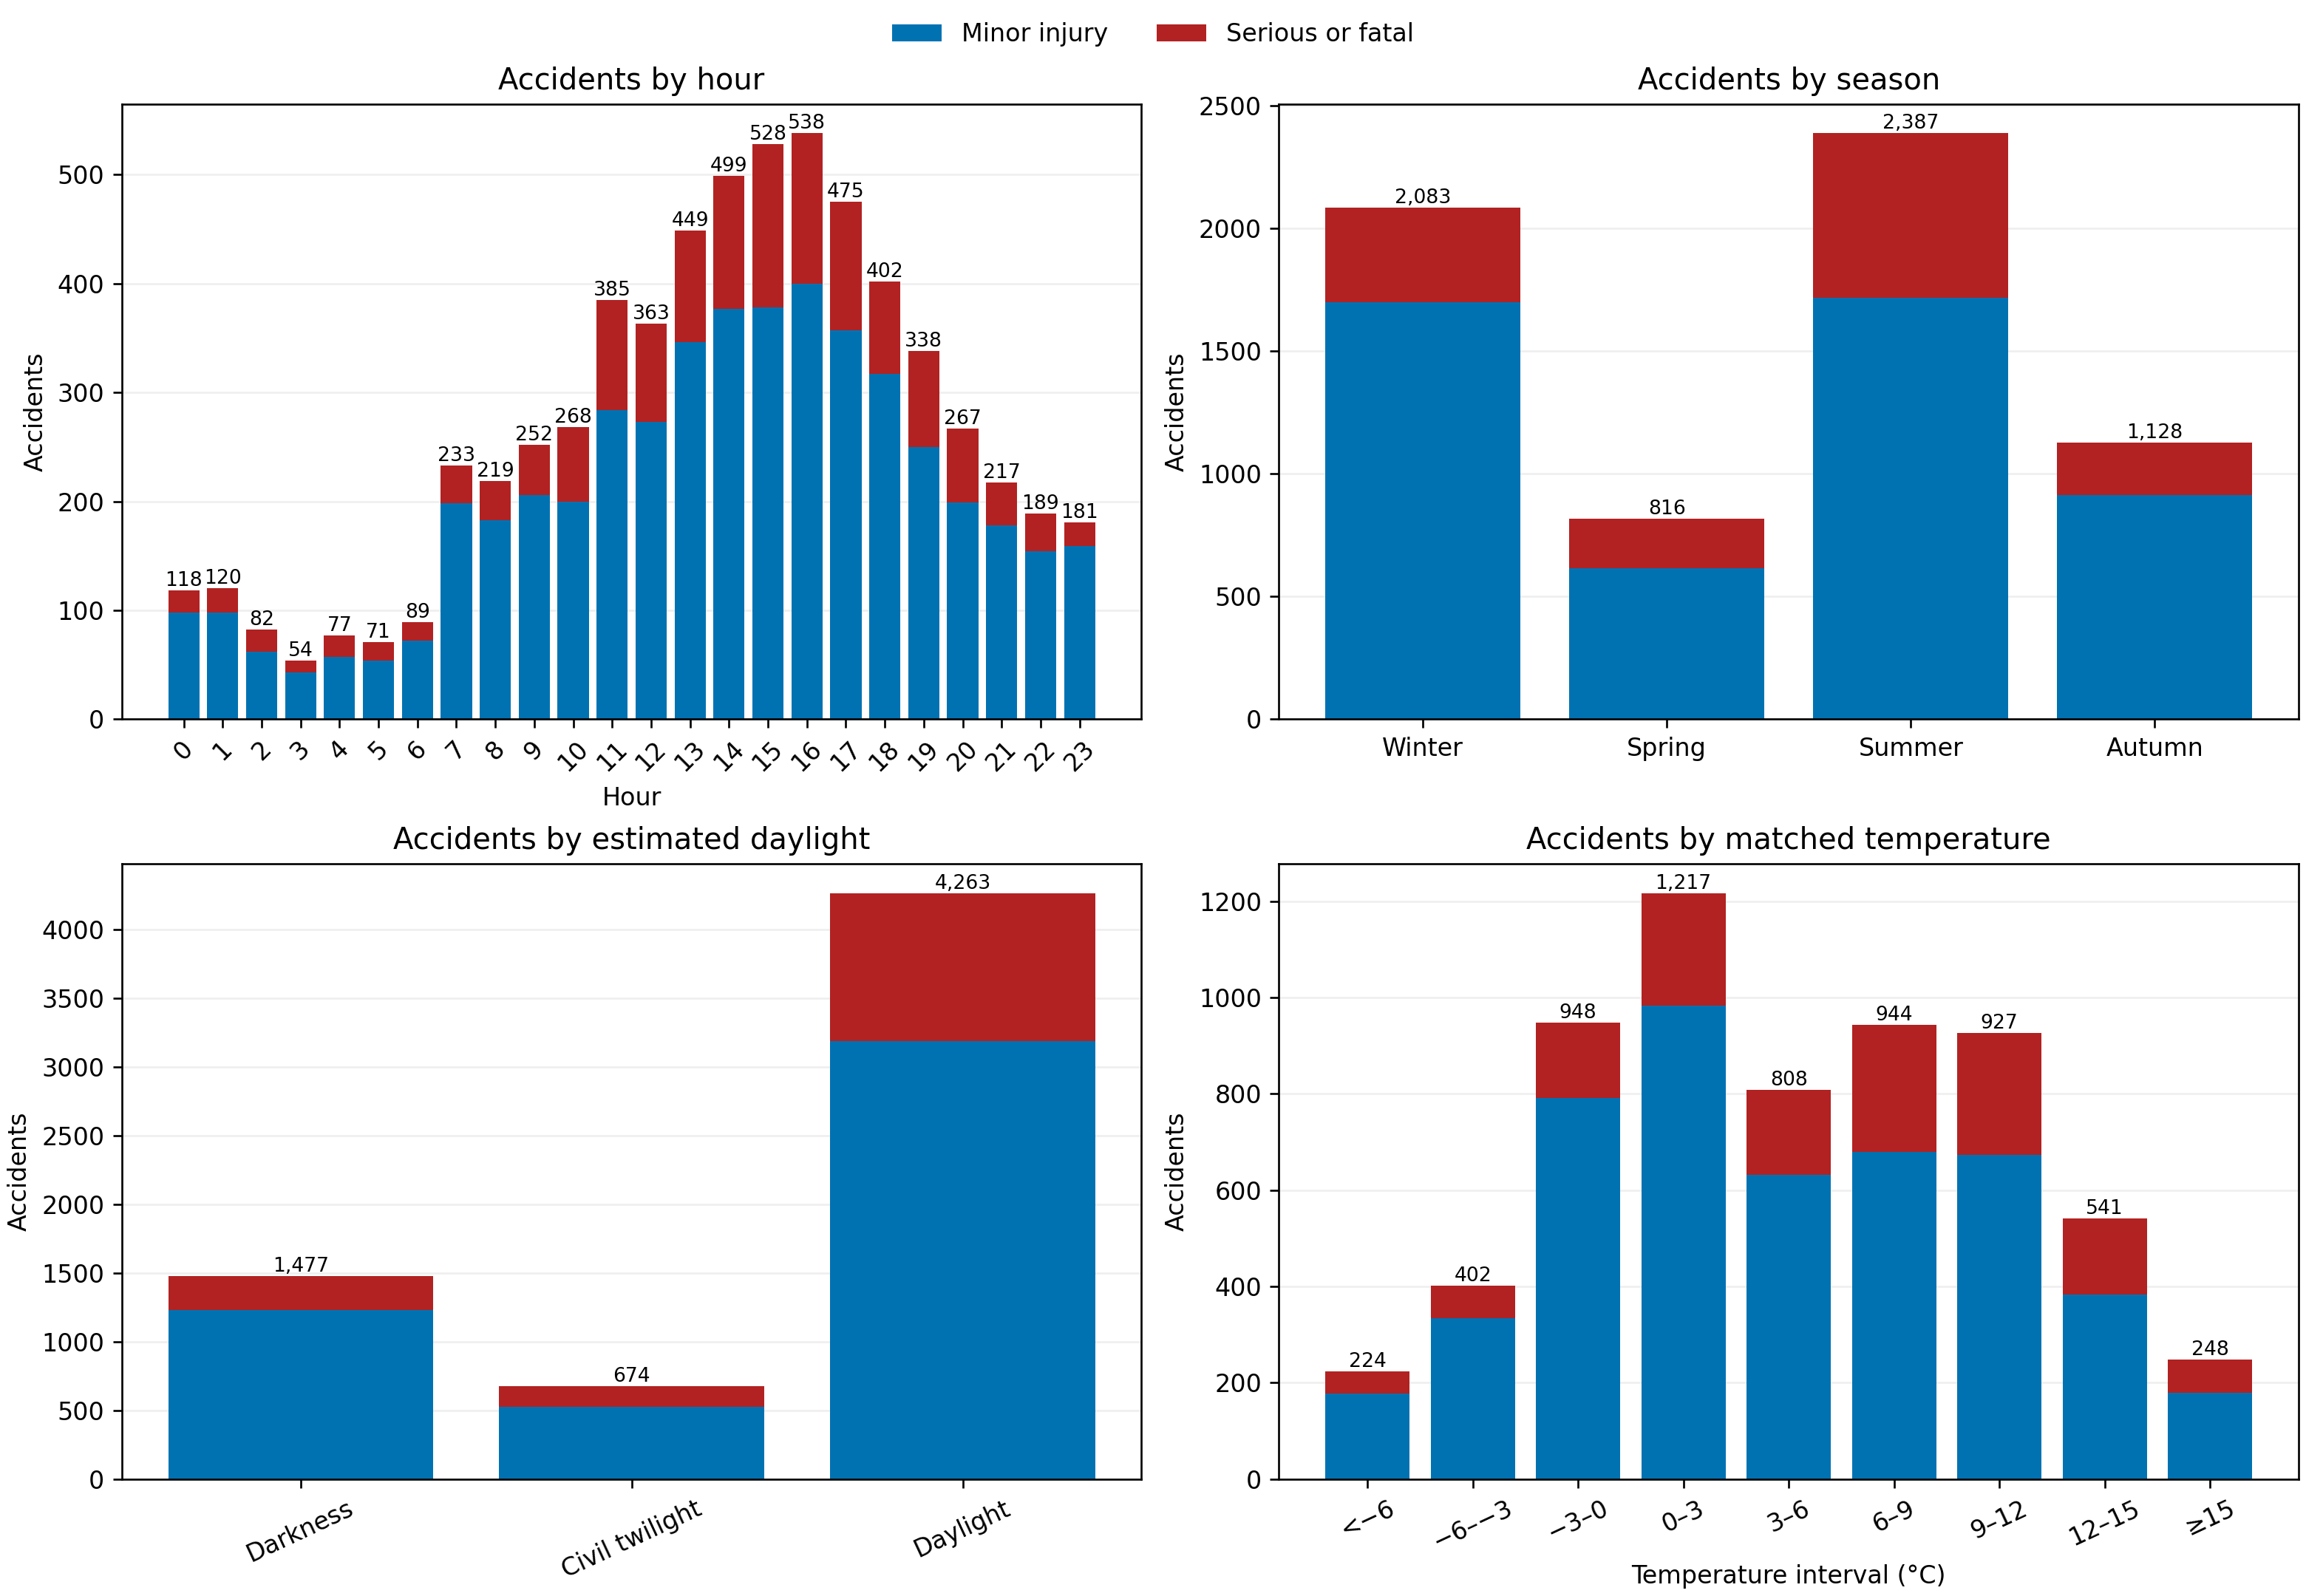
\includegraphics[width=\textwidth]{conditions.png}
\caption[Rural injury accidents by hour, season, daylight, and temperature.]{Rural injury accidents by hour, study season, estimated daylight
and matched temperature. Blue shows minor injury (code 3), and red shows
serious or fatal injury (codes 1--2). Labels give total accidents. Hour,
season and daylight use 6,414 accidents; temperature uses 6,259 qualifying
matches. These are descriptive counts, without traffic adjustment.}
\label{fig:accident-conditions}
\end{figure}

\section{Data Preparation and Reproducibility}

Table~\ref{tab:analysis-pipeline} summarises the path from source data to the
three main analyses. Accident, weather and traffic records first undergo
quality checks and selection. Qualifying accidents are matched to nearby
weather observations, and local weather frequencies form the denominator for
Q1. Q2 applies an approximate traffic correction estimated from the 2019--2024
counters to that same weather-frequency framework. Q3 uses the counter-linked
2019--2024 sample to estimate vehicle-kilometre exposure from observed daily
traffic, road length and pooled monthly weather frequencies. Matched-time and
additional traffic models are retained as supporting checks. This separation is important because the analyses use different
exposure assumptions and eligible samples.

All cleaning, matching, analysis, and thesis-table generation are scripted.
Generated tables are written from analysis outputs, and validation checks cover
key sample counts, matching rules, and exposure conservation. This reduces
manual transcription between the analysis and the thesis while keeping the
main transformations auditable.

\begin{table}[H]

\centering
\footnotesize
\setlength{\tabcolsep}{2.5pt}
\renewcommand{\arraystretch}{1.08}
\caption{Data preparation and analysis workflow.}
\label{tab:analysis-pipeline}
\begin{tabularx}{\textwidth}{L{0.16\textwidth}L{0.27\textwidth}L{0.27\textwidth}L{0.18\textwidth}}
\toprule
Stage & Main data & Output & Role in thesis \\
\midrule
Data preparation &
Accident, weather, road and traffic data &
Prepared analysis datasets &
Defines the study data. \\ \grayhline
Accident selection &
Accident data and urban boundaries &
Rural injury accidents &
Defines the study population. \\ \grayhline
Weather matching &
Accidents, weather observations and stations &
Accident-time weather and local frequencies &
Common input to the weather analyses. \\ \grayhline
Weather-frequency O/E &
Accident weather and local frequencies &
Observed and expected counts &
First analysis stage. \\ \grayhline
Approximate traffic-corrected O/E &
Primary O/E and 2019--2024 counter response &
Traffic-corrected expected counts &
Second analysis stage. \\ \grayhline
Monthly-frequency VKT analysis &
Recorded counter-days, rural lengths and monthly weather frequencies &
Accidents per million vehicle-km &
Third analysis stage. \\ \grayhline
Supporting analyses &
Matched control times and alternative traffic panels &
Matched odds ratios and alternative rate estimates &
Robustness checks. \\
\bottomrule
\end{tabularx}
\end{table}


\section{Analysis}

\subsection{Q1: Weather-Frequency Comparison}
\label{sec:weather-frequency}

Accident-time mean wind speed \texttt{f} is the main weather
measure and is divided into 5 m/s intervals. It is the 10-minute mean wind
observation matched within five minutes of the accident time, not an
instantaneous measurement. Wind gust \texttt{fg} from the same observation and
independently matched temperature are additional weather measures. For each
measure, accidents are compared with the distribution of that weather measure at
the matched station in the same study season, pooled across
all study years. Expected counts are therefore based on how often each
condition occurred locally rather than on a national weather distribution.
For example, if 5\% of the relevant station--season observations fall in one
wind interval, approximately 5\% of that group's accidents would be expected
there under weather-frequency-proportional occurrence.

Let \(g\) identify a weather station and study season.
Let \(A_{jg}\) be the number of accidents in weather interval \(j\) and group \(g\),
and let \(A_g=\sum_j A_{jg}\). From all quality-controlled 10-minute observations, let
\(T_{jg}\) be the number in interval \(j\) and \(T_g\) the total in group \(g\).
The local background frequency is

\[
p_{jg}=\frac{T_{jg}}{T_g}.
\]

If accident timing followed local wind frequency, the expected number in the
interval would be \(A_g p_{jg}\). The pooled observed/expected ratio is

\[
R_j=
\frac{\sum_g A_{jg}}
     {\sum_g A_g p_{jg}}.
\]

At mean wind of at least 20 m/s, 56 minor-injury accidents were observed
compared with 25.18 expected, giving O/E 2.22. This illustrates the calculation
without attributing any individual accident to wind.

A value of one means that the accident share equals the local time share of the
weather interval. A value above one means that accidents are over-represented
in that interval. Standardisation within station and season prevents locations
or seasons with different weather distributions from dominating the result.

The figures show the calculation separately for minor-injury accidents
(\textit{meiðsli}\(=3\)) and serious or fatal accidents
(\textit{meiðsli}\(\leq2\)). These groups do not overlap. Each group's
expected count uses its own accident totals within station and season.
The combined all-injury O/E is also retained for comparison with the other
analyses; it is calculated from summed observed and expected counts, not by
averaging the two group ratios. Q1 is reported as a descriptive standardised
ratio rather than a fitted inferential model, so observed and expected counts are
shown without model-based confidence intervals. Wind gust and temperature are
handled in the same way as mean wind. Temperature is
matched independently, and its intervals are below \(-6\), \(-6\) to \(-3\),
\(-3\) to 0, 0 to 3, 3 to 6, 6 to 9, 9 to 12, and at least
12\(^{\circ}\)C.
The O/E upper interval is combined at 12\(^{\circ}\)C to keep the seasonal
panels readable. The matched-time and annual-traffic models retain separate
12--15 and at-least-15\(^{\circ}\)C intervals. Estimates across those different
upper intervals are not treated as direct numerical comparisons.

\subsection{Use of Traffic Data}

The primary O/E denominator is the local frequency of wind conditions rather
than traffic volume. Complete traffic data are unavailable at the required
spatial and temporal resolution, so Q1 does not account for changes in travel
volume during strong wind. If traffic is lower in strong wind while other
factors remain unchanged, the accident-rate contrast per vehicle-kilometre
would be larger than the weather-frequency O/E contrast.

Traffic enters the main analysis in two ways. Q2 estimates the relative daily
traffic response across weather intervals from the 2019--2024 counters and uses
that response to reweight the Q1 denominator. Q3 constructs estimated
vehicle-kilometre exposure from observed daily traffic and rural road length in
a smaller counter-linked sample. Neither analysis observes hourly traffic.
Additional annual road-section and allocated daily-counter models are retained
as supporting checks under alternative exposure constructions.

\subsection{Q2: Approximate Traffic Correction to O/E}

The approximate correction uses the observed day-to-day traffic response at
counter sections during 2019--2024. Among positive-count days, the mean count
for the same counter section, year, month, and weekday defines expected daily
traffic. Each day's observed 24-hour count and expected count are allocated
to weather intervals in proportion to their valid 07:00--24:00 weather minutes
on that date. For interval \(j\), \(r_j\) is the sum of allocated observed
traffic divided by the sum of allocated expected traffic. Zero-count days are
excluded from this response calculation.

Using the same station--season group \(g\) and weather interval \(j\) as in Q1,
the traffic-weighted weather frequency is

\[
p^{*}_{jg}=\frac{p_{jg}r_j}{\sum_h p_{hg}r_h}.
\]

Expected counts are then recalculated as \(A_g p^{*}_{jg}\). Accident bins use
weather at the recorded accident time, whereas \(r_j\) is based on a 24-hour
traffic total repeated across the day's daytime weather composition. Daily
counters do not observe hourly traffic. The 2019--2024 response is also
extrapolated to the 2007--2025 primary population. The result is therefore a
model-based sensitivity analysis, not a directly observed traffic-adjusted O/E.

The period sensitivity repeats the original comparison separately for
2007--2018 and 2019--2024, restricting both accidents and background weather
to the stated years. The latter period is also recalculated with the counter
traffic response. These All year comparisons show what changes when the
accident and weather period aligns with the traffic data. Minor and serious
or fatal injuries remain disjoint and use their own expected counts. The
existing counter-era correction includes temperature as well as wind and gust;
it does not extend the full-period correction to temperature.

\subsection{Q3: Traffic-Based Accident Rates}

The main traffic rate is restricted to 2019--2024, when daily counter data are
available. Eligible accidents must be rural injury accidents occurring between
07:00 and 24:00, have a counter section for the registered road and year, be
successfully located on that section, have usable accident-time wind and gust
within 20 km and five minutes, and have a traffic record on the accident date.
For this analysis, the 20 km weather distance is measured from the
counter-section location rather than from the accident coordinate. The same
five-minute time rule applies as in Q1 and can select the adjacent observation
across midnight. The denominator is broader than the accident set: it uses
every eligible recorded counter-section day with a nonnegative traffic count
and rural road length, including days without an accident. For counter section
\(j\), date \(d\), and weather interval \(b\), estimated exposure, in vehicle-kilometres travelled (VKT), is

\[
\widehat V_{jdb}=C_{jd}L_jp_{j,m(d),b},
\]

where \(C_{jd}\) is the observed 24-hour traffic count, \(L_j\) is rural
section length under that year's definition, and \(p_{j,m(d),b}\) is the
07:00--24:00 weather frequency for that calendar month at the station assigned
to counter section \(j\). The weather frequencies are pooled across 2007--2025 to provide stable
station--month proportions, while both traffic and accident eligibility remain
restricted to 2019--2024. The full daily count is allocated to the 07:00--24:00
window and the proportions sum to one, so exposure is conserved. Accidents are
classified separately by observed event-time weather within 20 km and five
minutes. The reported rate is

\[
R_b=\frac{O_b}{\sum_j\sum_d\widehat V_{jdb}}10^6.
\]

This construction uses actual day-to-day traffic variation and rural road
length, but allocates it with a typical monthly weather distribution rather
than observed hourly traffic. Daily traffic still varies from day to day, but
one storm day's weather does not determine that day's entire allocation among
weather bins. The typical distribution for the station and calendar month
provides a more stable allocation. This is an exposure assumption, not evidence
that the monthly method measures actual traffic within each weather interval.

For the injury-component figures, the exposure denominator
\(\widehat V_b=\sum_j\sum_d\widehat V_{jdb}\) is shared:
\[
R_b^{\mathrm{minor}}=\frac{O_b^{\mathrm{minor}}}{\widehat V_b}10^6,
\qquad
R_b^{\mathrm{serious/fatal}}=\frac{O_b^{\mathrm{serious/fatal}}}{\widehat V_b}10^6.
\]
Minor injury means code 3; serious or fatal injury means codes 1--2. Their
counts are disjoint, so their rates sum to the all-injury rate. Blue forms
the bottom of each stack and red the top. This is a descriptive decomposition
of the accident numerator, not a severity model. For seasonal panels, counts
and exposure are summed within each study season before division; the seasons
partition the All year result. In the seasonal rate figures, mean-wind
intervals at or above 15 m/s and gust intervals at or above 20 m/s are combined
by summing counts and exposure before division. All year retains the fine bins.

\paragraph{Same-day allocation sensitivity.}
The alternative allocation uses weather observed on each actual counter-day:
\[
\widehat V^{\mathrm{day}}_b=\sum_j\sum_d C_{jd}L_j
\frac{M_{jdb}}{1020},
\qquad
R^{\mathrm{day}}_b=\frac{O_b}{\widehat V^{\mathrm{day}}_b}10^6,
\]
where \(M_{jdb}\) is the number of observed minutes in bin \(b\) during
07:00--24:00. Traffic is assumed uniform over this window. Weather is taken
from the nearest qualifying station available at each timestamp; missing
weather time contributes no allocated exposure. Eligible positive-traffic days
without accidents still contribute. Unlike monthly allocation, this method
retains only weather-covered exposure rather than the full daily total. It therefore depends more strongly on the weather
composition of individual days, completeness of observations and the assumption
about traffic within the day. Sparse extreme-weather days can have greater
influence. It is retained as a sensitivity, not a replacement for the main
monthly-frequency denominator.
The accident numerator still uses actual event-time weather in the linked
sample. The existing output supports mean wind, gust and temperature, with
disjoint injury groups sharing exposure in each bin and season. Seasonal wind
and gust tails are combined for display as specified in Results, while All year
keeps the finer bins. This is Q3's exposure-allocation sensitivity, distinct
from the older allocated daily-counter regression below.

Table~\ref{tab:allocation-comparison} summarises the two exposure constructions.
Monthly allocation is the main method because only daily traffic totals are
observed: typical station-month weather provides a stable allocation while
retaining actual day-to-day traffic variation. It depends less on isolated
storm days and missing observations within a particular day. Same-day allocation
has the useful advantage of using realised weather, but distributing the full
daily traffic total using that day's observed weather requires an additional
assumption about traffic within the day. Neither method observes hourly exposure.

\begin{table}[htbp]
\centering
\small
\caption{Comparison of the main monthly-frequency allocation and same-day sensitivity.}
\label{tab:allocation-comparison}
\begin{tabularx}{\textwidth}{@{}>{\raggedright\arraybackslash}p{0.20\textwidth}>{\raggedright\arraybackslash}X>{\raggedright\arraybackslash}X@{}}
\hline
 & \textbf{Monthly-frequency main method} & \textbf{Same-day sensitivity} \\
\hline
Traffic and road input & Observed daily count $\times$ rural road length & Same \\
Weather allocation & Typical pooled station-month distribution & Weather observed on the actual date \\
Accident classification & Actual accident-time weather & Actual accident-time weather \\
Accident-free days & Included when eligible & Included where weather defines exposure \\
Hourly traffic observed? & No & No \\
Main advantage & Stable weather-bin allocation & Responds to realised daily weather \\
Key limitation & Monthly weather approximates exposure & Daily total allocated by observed weather; missing time excluded \\
Role & Main traffic-rate analysis & Sensitivity to allocation choice \\
\hline
\end{tabularx}
\end{table}

\subsection{Supporting Matched-Time Comparison}

The supporting matched-time analysis uses a time-stratified case-crossover
design in which each accident forms one matched set. The accident time is the
case time, and the control times are the other occurrences of the same weekday
and clock time in the same calendar month and year. For example, a
Tuesday accident at 14:20 is compared with the other Tuesdays at 14:20 in that
month. Mean-wind and gust controls use the accident's matched wind station;
temperature controls use its independently matched temperature station. Control
weather must satisfy the same five-minute observation-time rule, and both station
matches are restricted to 20 km. Conditional logistic regression compares
weather at the accident time with weather at its matched control times. This
time-stratified referent strategy was selected to avoid overlap bias and to
control calendar time without selecting controls from outside the accident
month \citep{janes2005}.

The model asks whether weather at an accident time differs from weather at
comparable non-accident times. The matching holds station, year, month, weekday,
and clock time fixed, but not unusual traffic, road conditions, or other
factors that change on a particular day. Continuous effects are reported per
5 m/s or 5\(^{\circ}\)C together with categorical estimates.

Mean wind and temperature are also entered together as categorical variables
to assess whether the wind estimate changes after including temperature at the
same case and control times. Daylight is calculated at the accident location for the accident date and the same matched
dates. Because month, weekday, and clock time are held fixed, only strata that
change between darkness, civil twilight, and daylight contribute information.

Seasonal differences in the mean-wind association are tested in a separate
matched-time model. Mean wind is grouped as 0--10, 10--15, and at least
15 m/s for stability. The model includes interactions between wind interval and
season, and a likelihood-ratio test compares it with a model having one common
wind association across seasons. The omnibus test is used instead of judging
seasonal differences from separate confidence intervals.

A separate logistic model describes serious or fatal rather than minor injury
among accidents with complete wind and temperature matches. It includes broad
categories of mean wind, temperature, daylight, time of day, and season. The
result concerns injury severity among recorded accidents. It is not a model of
whether an accident occurs and does not replace the traffic analyses.

\subsection{Supporting Road-Section Traffic Comparison}

Annual road-section data provide a supporting exposure analysis for accidents
that can be linked by road section, year, official traffic period, and wind
interval. For road-section--year--traffic-period stratum \(k\) and wind
interval \(j\), estimated vehicle-kilometres are

\[
V_{kj}=q_k L_k D_k p_{kj},
\]

where \(q_k\) is SDU, VDU, or derived VHDU vehicles per day, \(L_k\) is section
length, \(D_k\) is the number of calendar days, and \(p_{kj}\) is the local
share of quality-controlled 10-minute observations in wind interval \(j\).
This construction accounts for road length and differences in published
seasonal traffic, but assumes that traffic within each traffic period is
distributed across wind intervals in proportion to time. It does not observe
traffic at the accident minute.

The station nearest the road-section midpoint with qualifying data supplies
\(p_{kj}\). Accidents in this analysis are matched to that road-section station,
rather than to the accident-nearest station used in Q1, and are retained only
when the station is within 20 km and has a valid observation within five
minutes of the accident time.

A conditional Poisson model is fitted as a supporting inferential analysis.
Each road section, year, and traffic period has its own intercept:

\[
\log E(A_{kj}) = \alpha_k + \beta_j + \log V_{kj},
\]

where \(A_{kj}\) is the accident count and \(\log V_{kj}\) is the offset. The
exponentiated coefficient \(\exp(\beta_j)\) is the estimated rate ratio relative
to 0--5 m/s within road-section--year--traffic-period strata. Strata with no
accidents contain no within-stratum information after conditioning and do not
contribute to this model. The model is fitted separately for all injury
accidents and for serious or fatal accidents. A seasonal extension uses
0--10, 10--15, and at least 15 m/s because the finer upper-wind cells are
sparse.

\subsection{Supporting Allocated Daily-Counter Model}

An additional daily-counter model uses observed 24-hour totals but estimates
how those totals are distributed across wind intervals within each day.
Directional channels are first summed to one count for each physical counter
and date. Each 2019--2024 accident then requires a counter on the exact
registered road section and year, positive traffic on the accident date, and a
qualifying accident-time mean-wind observation. For counter \(c\), date \(d\),
and wind interval \(j\), the daily count is allocated as

\[
\widehat Q_{cdj}=Q_{cd}\frac{N_{cdj}}{N_{cd}},
\]

where \(N_{cdj}\) is the number of valid 10-minute observations in interval
\(j\) and \(N_{cd}\) is the total number of valid observations that day.
Accidents are classified by accident-time mean wind from the same station used
for the counter-day denominator. Estimated traffic and accidents are aggregated
by counter, year, and wind interval, and a conditional Poisson model gives each
counter--year its own intercept. The allocation assumes uniform traffic across
valid observation times and is therefore an estimated within-day split rather
than observed hourly exposure. Selection and sensitivity checks for this
762-accident supporting model are reported in the appendix.

\chapter{Results}

Results are presented in the order of the three research questions. First, the
primary weather-frequency analysis compares observed accidents with counts
expected from local weather frequency. Second, an approximate traffic
correction asks how that comparison changes when the traffic response measured at daily
counters is applied to the primary denominator. Third, the monthly-frequency
counter analysis estimates accident rates per vehicle-kilometre in the smaller
2019--2024 traffic-linked sample. Matched-time and additional traffic models
are reported afterwards as supporting checks. Because these analyses use
different samples and denominators, their numerical estimates are not interpreted as
repeated estimates of the same quantity.

\section{Study Sample and Coverage}

Table~\ref{tab:coverage} summarises the populations used by the main and
supporting analyses. The primary O/E retains 6,259 of the 6,414 rural injury
accidents, whereas analyses requiring traffic linkage use smaller and more
selective samples. Figure~\ref{fig:annual-coverage} shows that weather-match
coverage remains high throughout 2007--2025.

\begin{table}[H]
\centering
\footnotesize
\caption[Analysis sample sizes.]{Accident selection and analysis sample sizes.}
\label{tab:coverage}
\begin{tabularx}{\textwidth}{L{0.34\textwidth}rX}
\toprule
Stage & Accidents & Purpose \\
\midrule
Source records & 126,607 & Accident database, 2007--2025. \\ \grayhline
Rural injury accidents & 6,414 & Study population. \\ \grayhline
Q1: Primary O/E & 6,259 & Main weather-frequency analysis. \\ \grayhline
Q2: Approximate traffic correction & 6,259 & Same accident sample as Q1; denominator reweighted using counter-derived traffic response. \\ \grayhline
Q3: Monthly-frequency VKT & 694 & Main counter-linked traffic analysis, 2019--2024. \\ \grayhline
Supporting matched-time & 6,257 & Time-matched robustness analysis. \\ \grayhline
Supporting annual traffic & 5,125 & Broader road-linked traffic model. \\ \grayhline
Supporting allocated daily-counter & 762 & Alternative daily-counter model. \\
\bottomrule
\end{tabularx}
\end{table}


\begin{figure}[htbp]
\centering
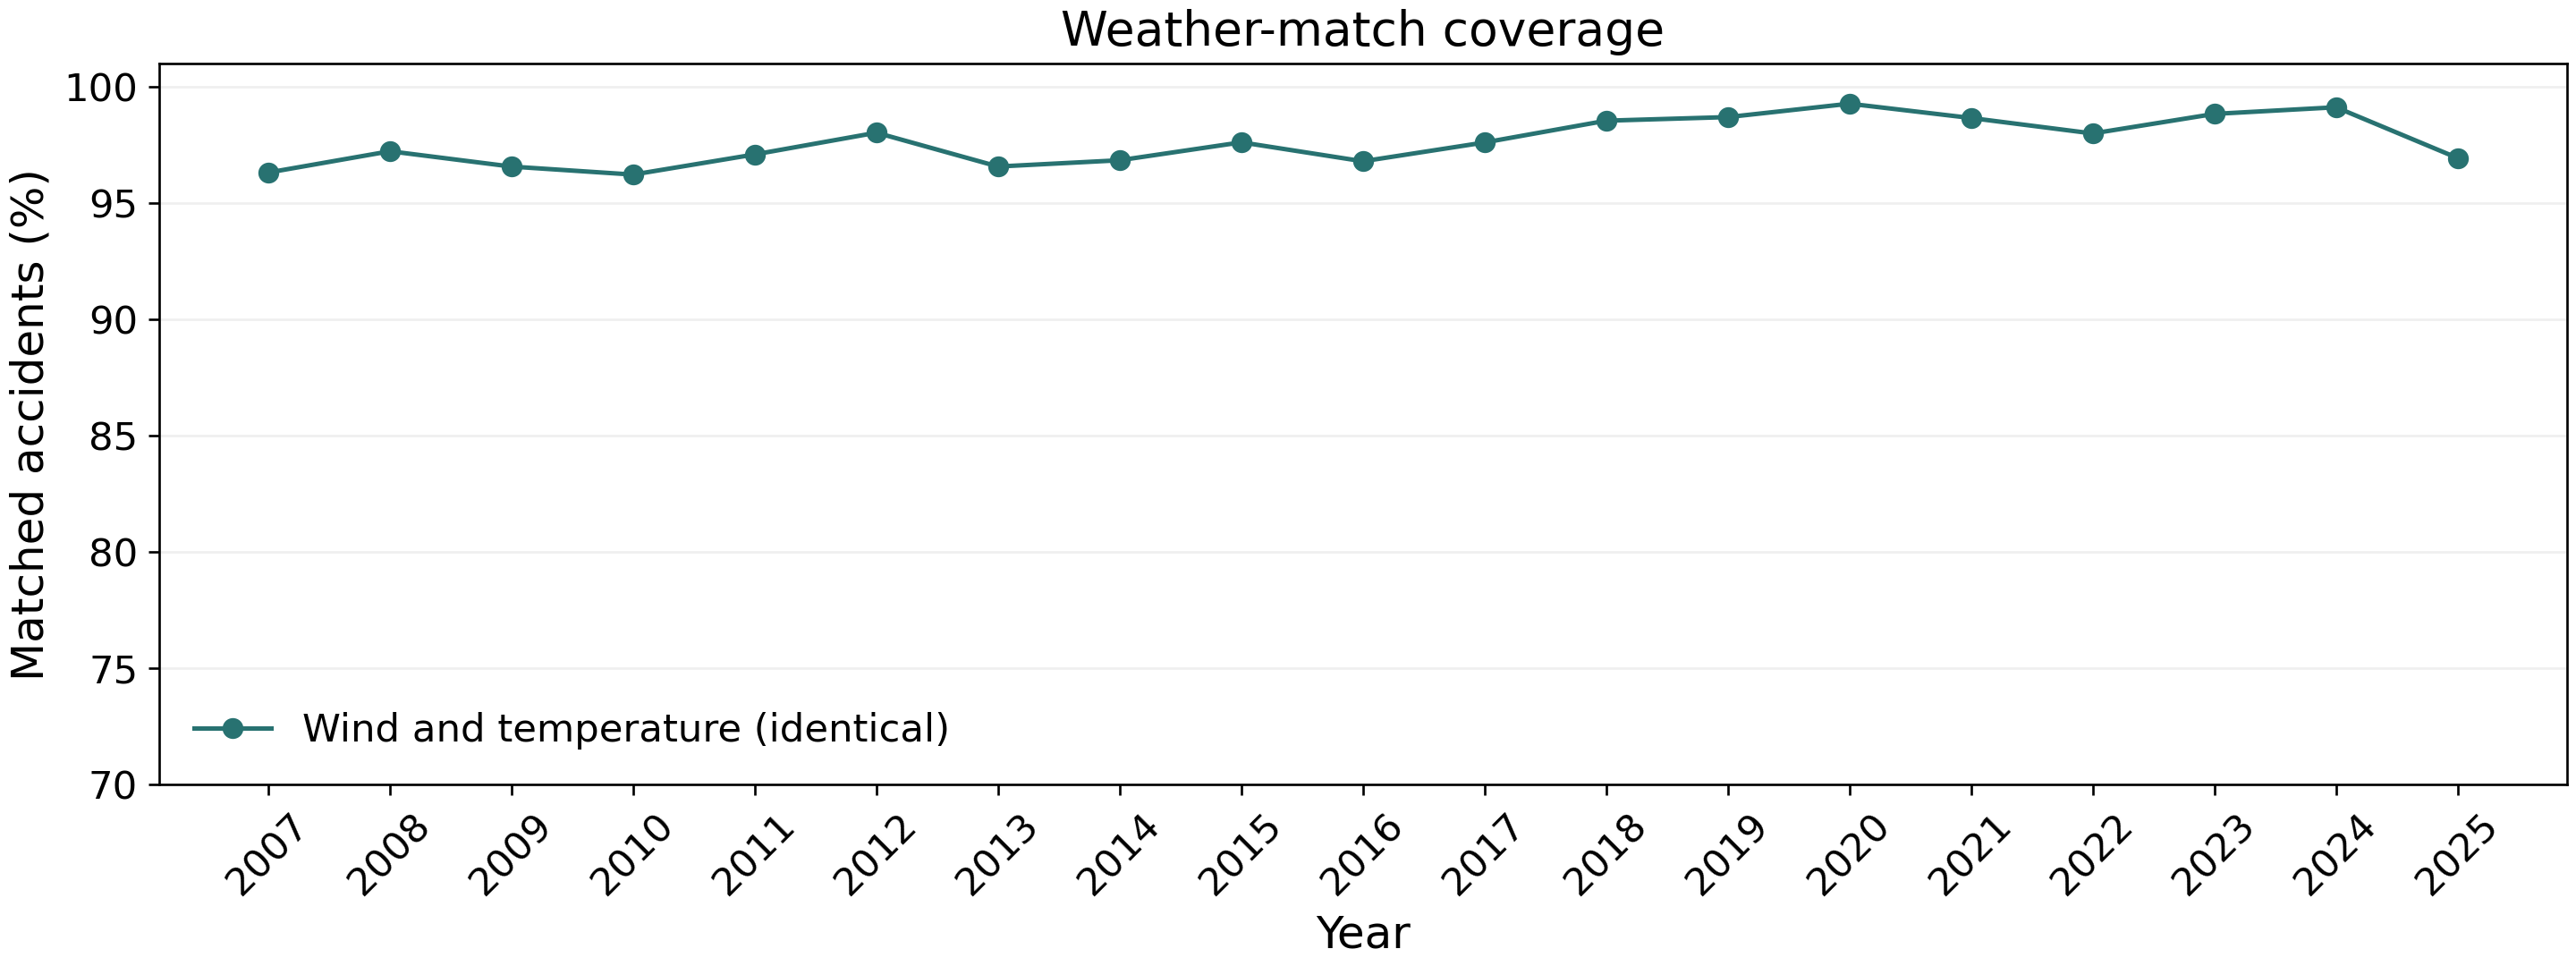
\includegraphics[width=0.9\textwidth]{weather_coverage.png}
\caption[Annual rural injury-accident counts and weather-match coverage.]{Annual rural injury-accident counts and weather-match coverage,
2007--2025. The lower panel gives the percentage of accidents with a qualifying
wind or temperature observation within 20 km and five minutes. Wind and
temperature coverage is identical in every year, and no missing temperature
value is imputed.}
\label{fig:annual-coverage}
\end{figure}

The 20 km threshold provides broad coverage while limiting the distance between
an accident and its weather proxy. It does not imply that station conditions
are identical to conditions at the road, particularly in complex terrain.
Wind and temperature are matched independently, but both procedures retain the
same accidents and select the same station and observation time in the
final analysis dataset.

Question 3 uses a different starting population because daily counters are
available only for 2019--2024. Table~\ref{tab:monthly-vkt-selection} shows the
full selection from all injury accidents in 2007--2025, first restricting to
2019--2024 and then applying the Q3 linkage criteria, to the final 694
counter-linked daytime accidents. The first row includes urban and rural injury
accidents; the rural restriction is applied in step~(a). All 83 exclusions at
the final step lack a counter-day record on the accident date; no accident is
removed because its recorded daily count is zero.

\begin{table}[htbp]
\centering
\caption{Selection for the monthly-frequency daily-counter rate. The final set contains all injury severities and is distinct from the earlier allocated daily samples.}
\label{tab:monthly-vkt-selection}
\small
\begin{tabular}{p{0.64\textwidth}rr}
\toprule
Step & Removed & Remaining \\ \midrule
All injury accidents, 2007-2025 & -- & 17,045 \\ \grayhline
0) Restrict to 2019-2024 & 11,849 & 5,196 \\ \grayhline
a) Exclude urban accidents & 3,333 & 1,863 \\ \grayhline
b) Require counter-section road/year & 994 & 869 \\ \grayhline
c) Require successful road-location assignment & 21 & 848 \\ \grayhline
d) Exclude 00:00-07:00 & 67 & 781 \\ \grayhline
e) Require usable wind and gust & 4 & 777 \\ \grayhline
Require daily traffic count & 83 & 694 \\ \grayhline
\bottomrule
\end{tabular}
\end{table}


\section{Weather-Frequency Baseline}

Figures~\ref{fig:wind-oe-panels}--\ref{fig:temperature-oe-panels} show the
primary weather-frequency comparisons for the full year and the four study
seasons. Blue bars show minor-injury accidents and red bars show serious or
fatal injury accidents; the groups do not overlap. The grey horizontal line
marks O/E = 1, where observed accidents equal the number expected from local
weather frequency. Values above one indicate over-representation relative to
that frequency, not a measured increase in risk per vehicle-kilometre.

\subsection{Mean Wind}

Figure~\ref{fig:wind-oe-panels} shows the main result: O/E is close to one
at low and moderate mean wind speeds and rises in the upper intervals.
At 20 m/s or above, the all-injury O/E is 2.15. Both injury groups show this
upper-wind pattern, but the serious or fatal group contains few accidents.
Differences between the bars should therefore not be read as evidence that
wind changes injury severity.

\begin{figure}[!htbp]
\centering
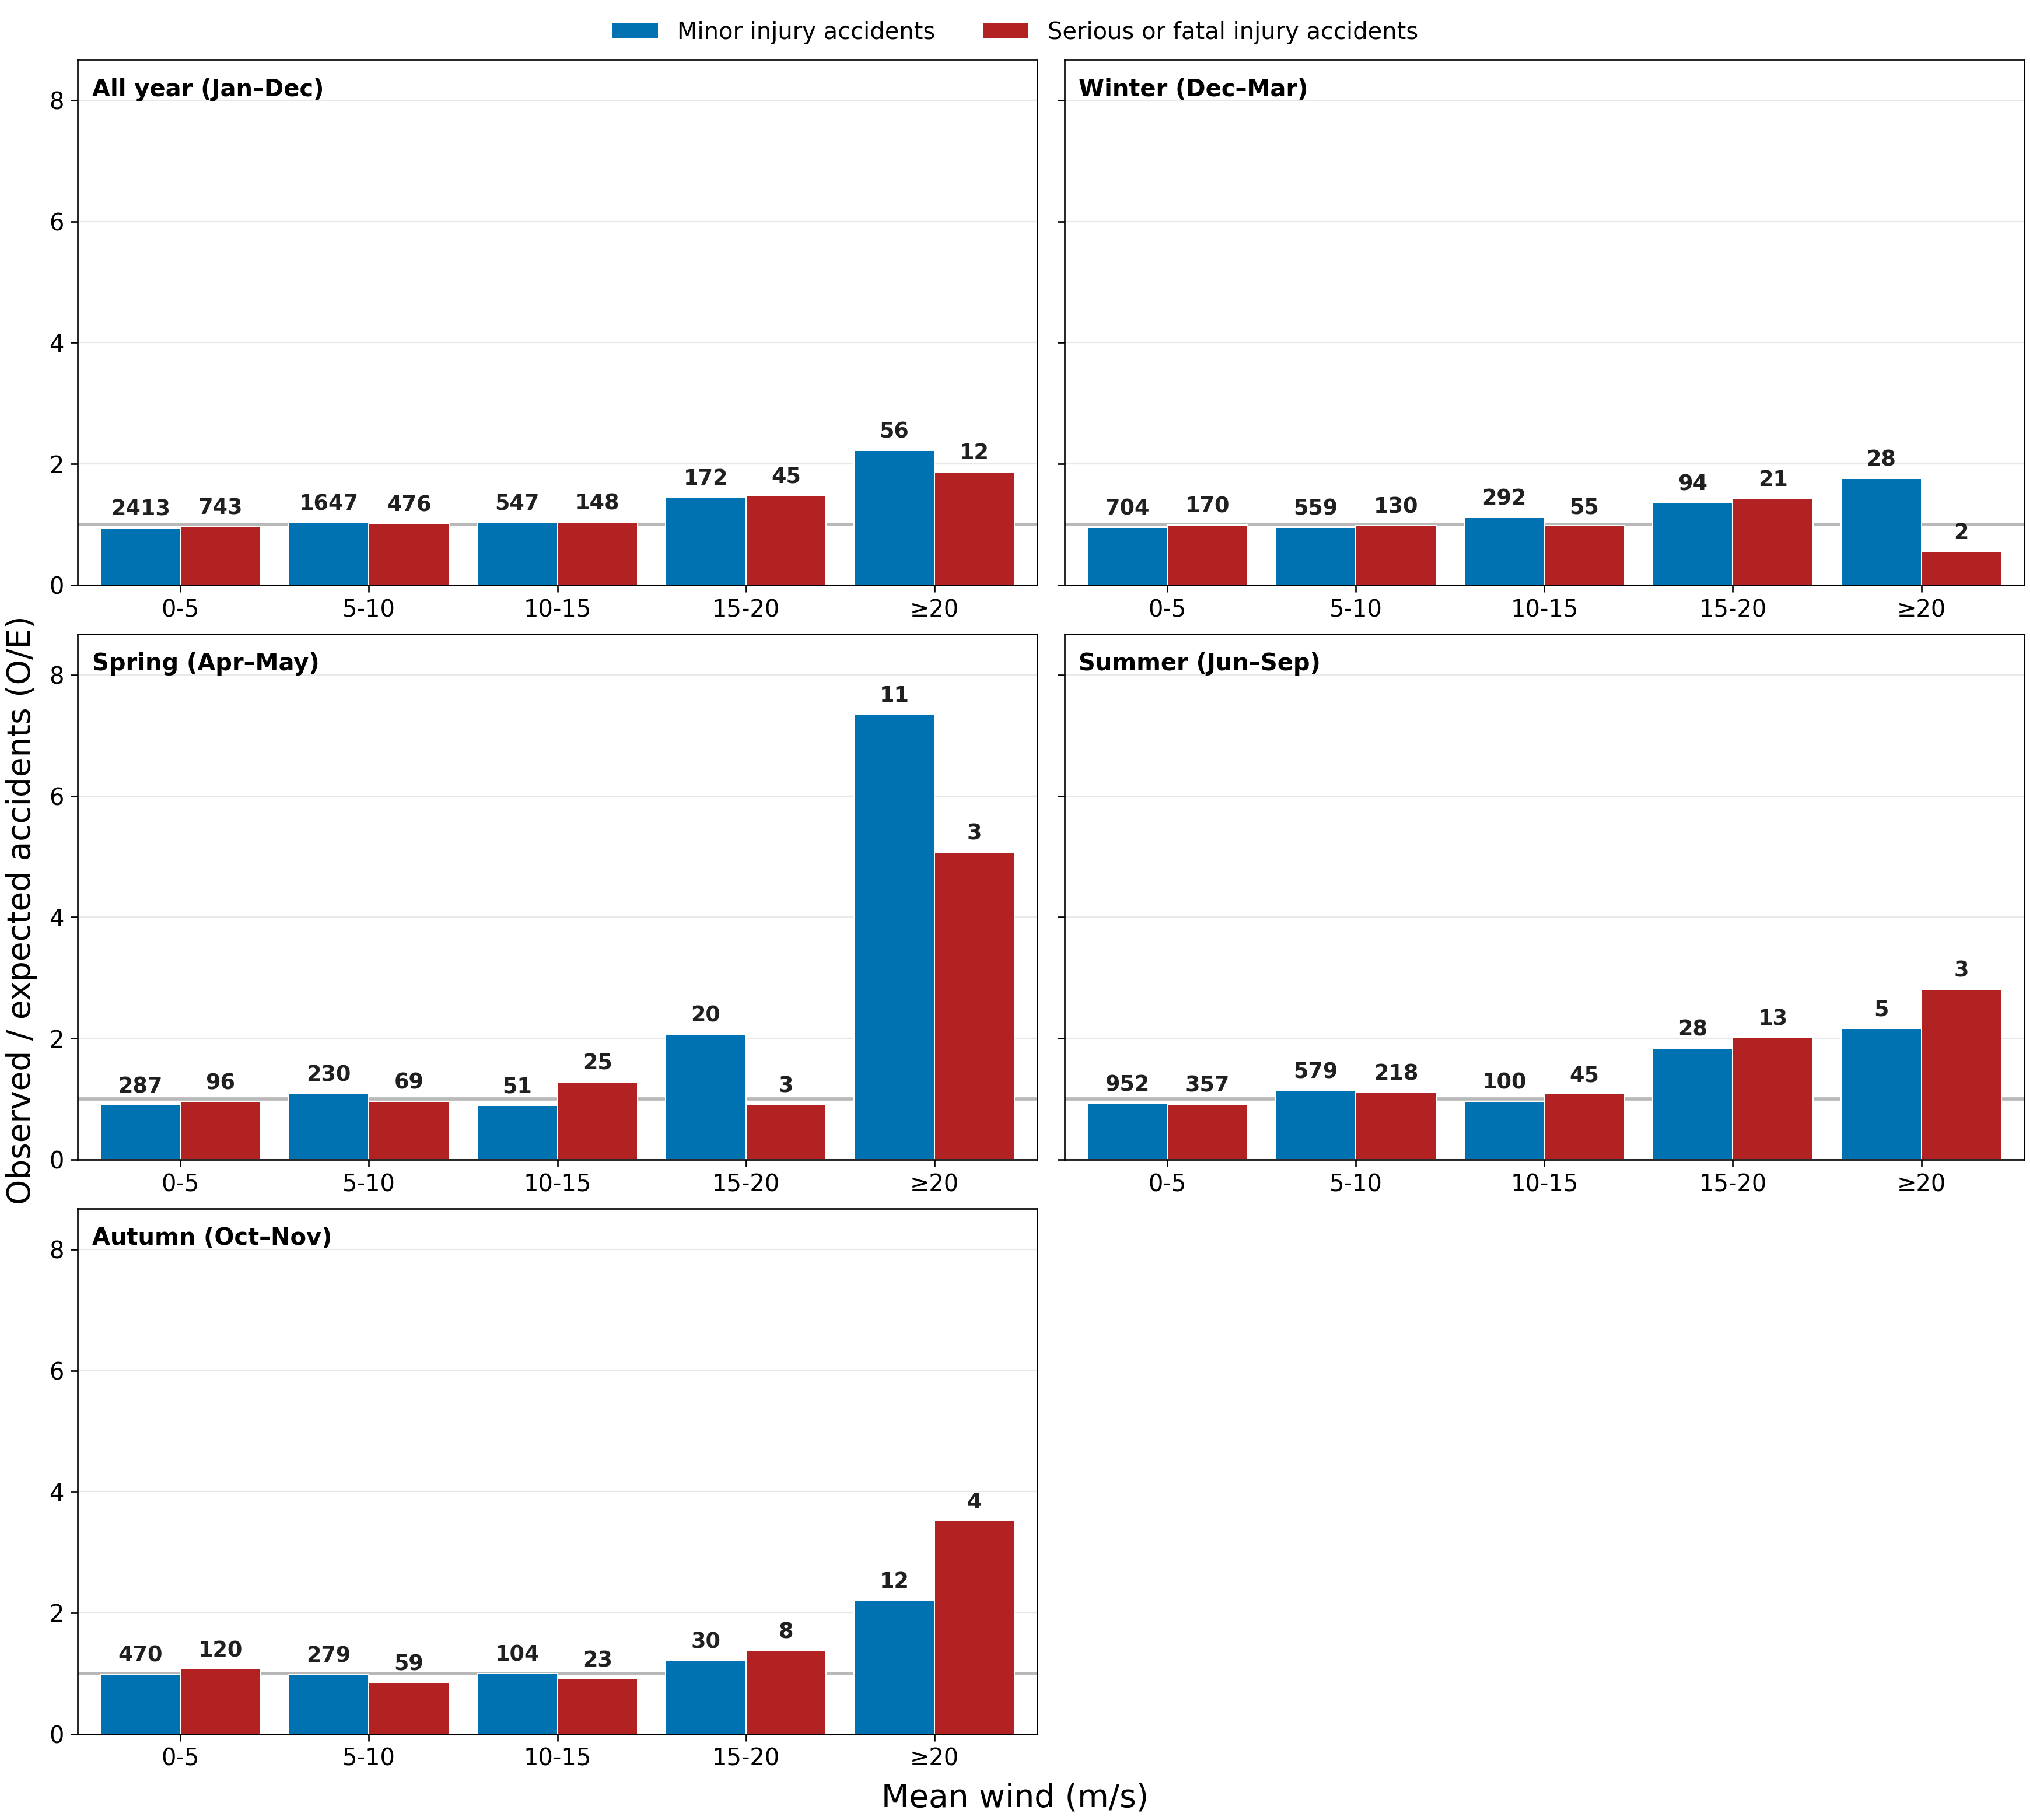
\includegraphics[width=\textwidth,height=0.82\textheight,keepaspectratio]{wind_oe_panels.png}
\caption[All-year and seasonal mean-wind O/E, 2007--2025.]{All-year and seasonal mean-wind O/E, 2007--2025. Blue bars show minor
injury and red bars show serious or fatal injury. Expected counts are calculated from local
station--season weather frequency separately for each group; labels above bars
are observed accident counts. The grey reference line is O/E = 1. Seasonal
upper-wind bars should be interpreted with their small observed counts.}
\label{fig:wind-oe-panels}
\end{figure}

The seasonal panels are less stable than the pooled result. In particular,
some of the largest seasonal O/E values are based on only a few accidents, so
they do not support ranking seasons or injury groups. The 5 m/s intervals are
used as descriptive bins rather than physical wind thresholds.

\subsection{Wind Gust}

Wind gust shows a similar upper-tail pattern in Figure~\ref{fig:gust-oe-panels},
with all-injury O/E 3.34 at gusts of at least 30 m/s. Both injury groups are
above one in this interval. Gust and mean wind are related measurements from
the same observation, so their agreement supports a general high-wind pattern
rather than an independent replication. Seasonal extremes remain sparse.

\begin{figure}[!htbp]
\centering
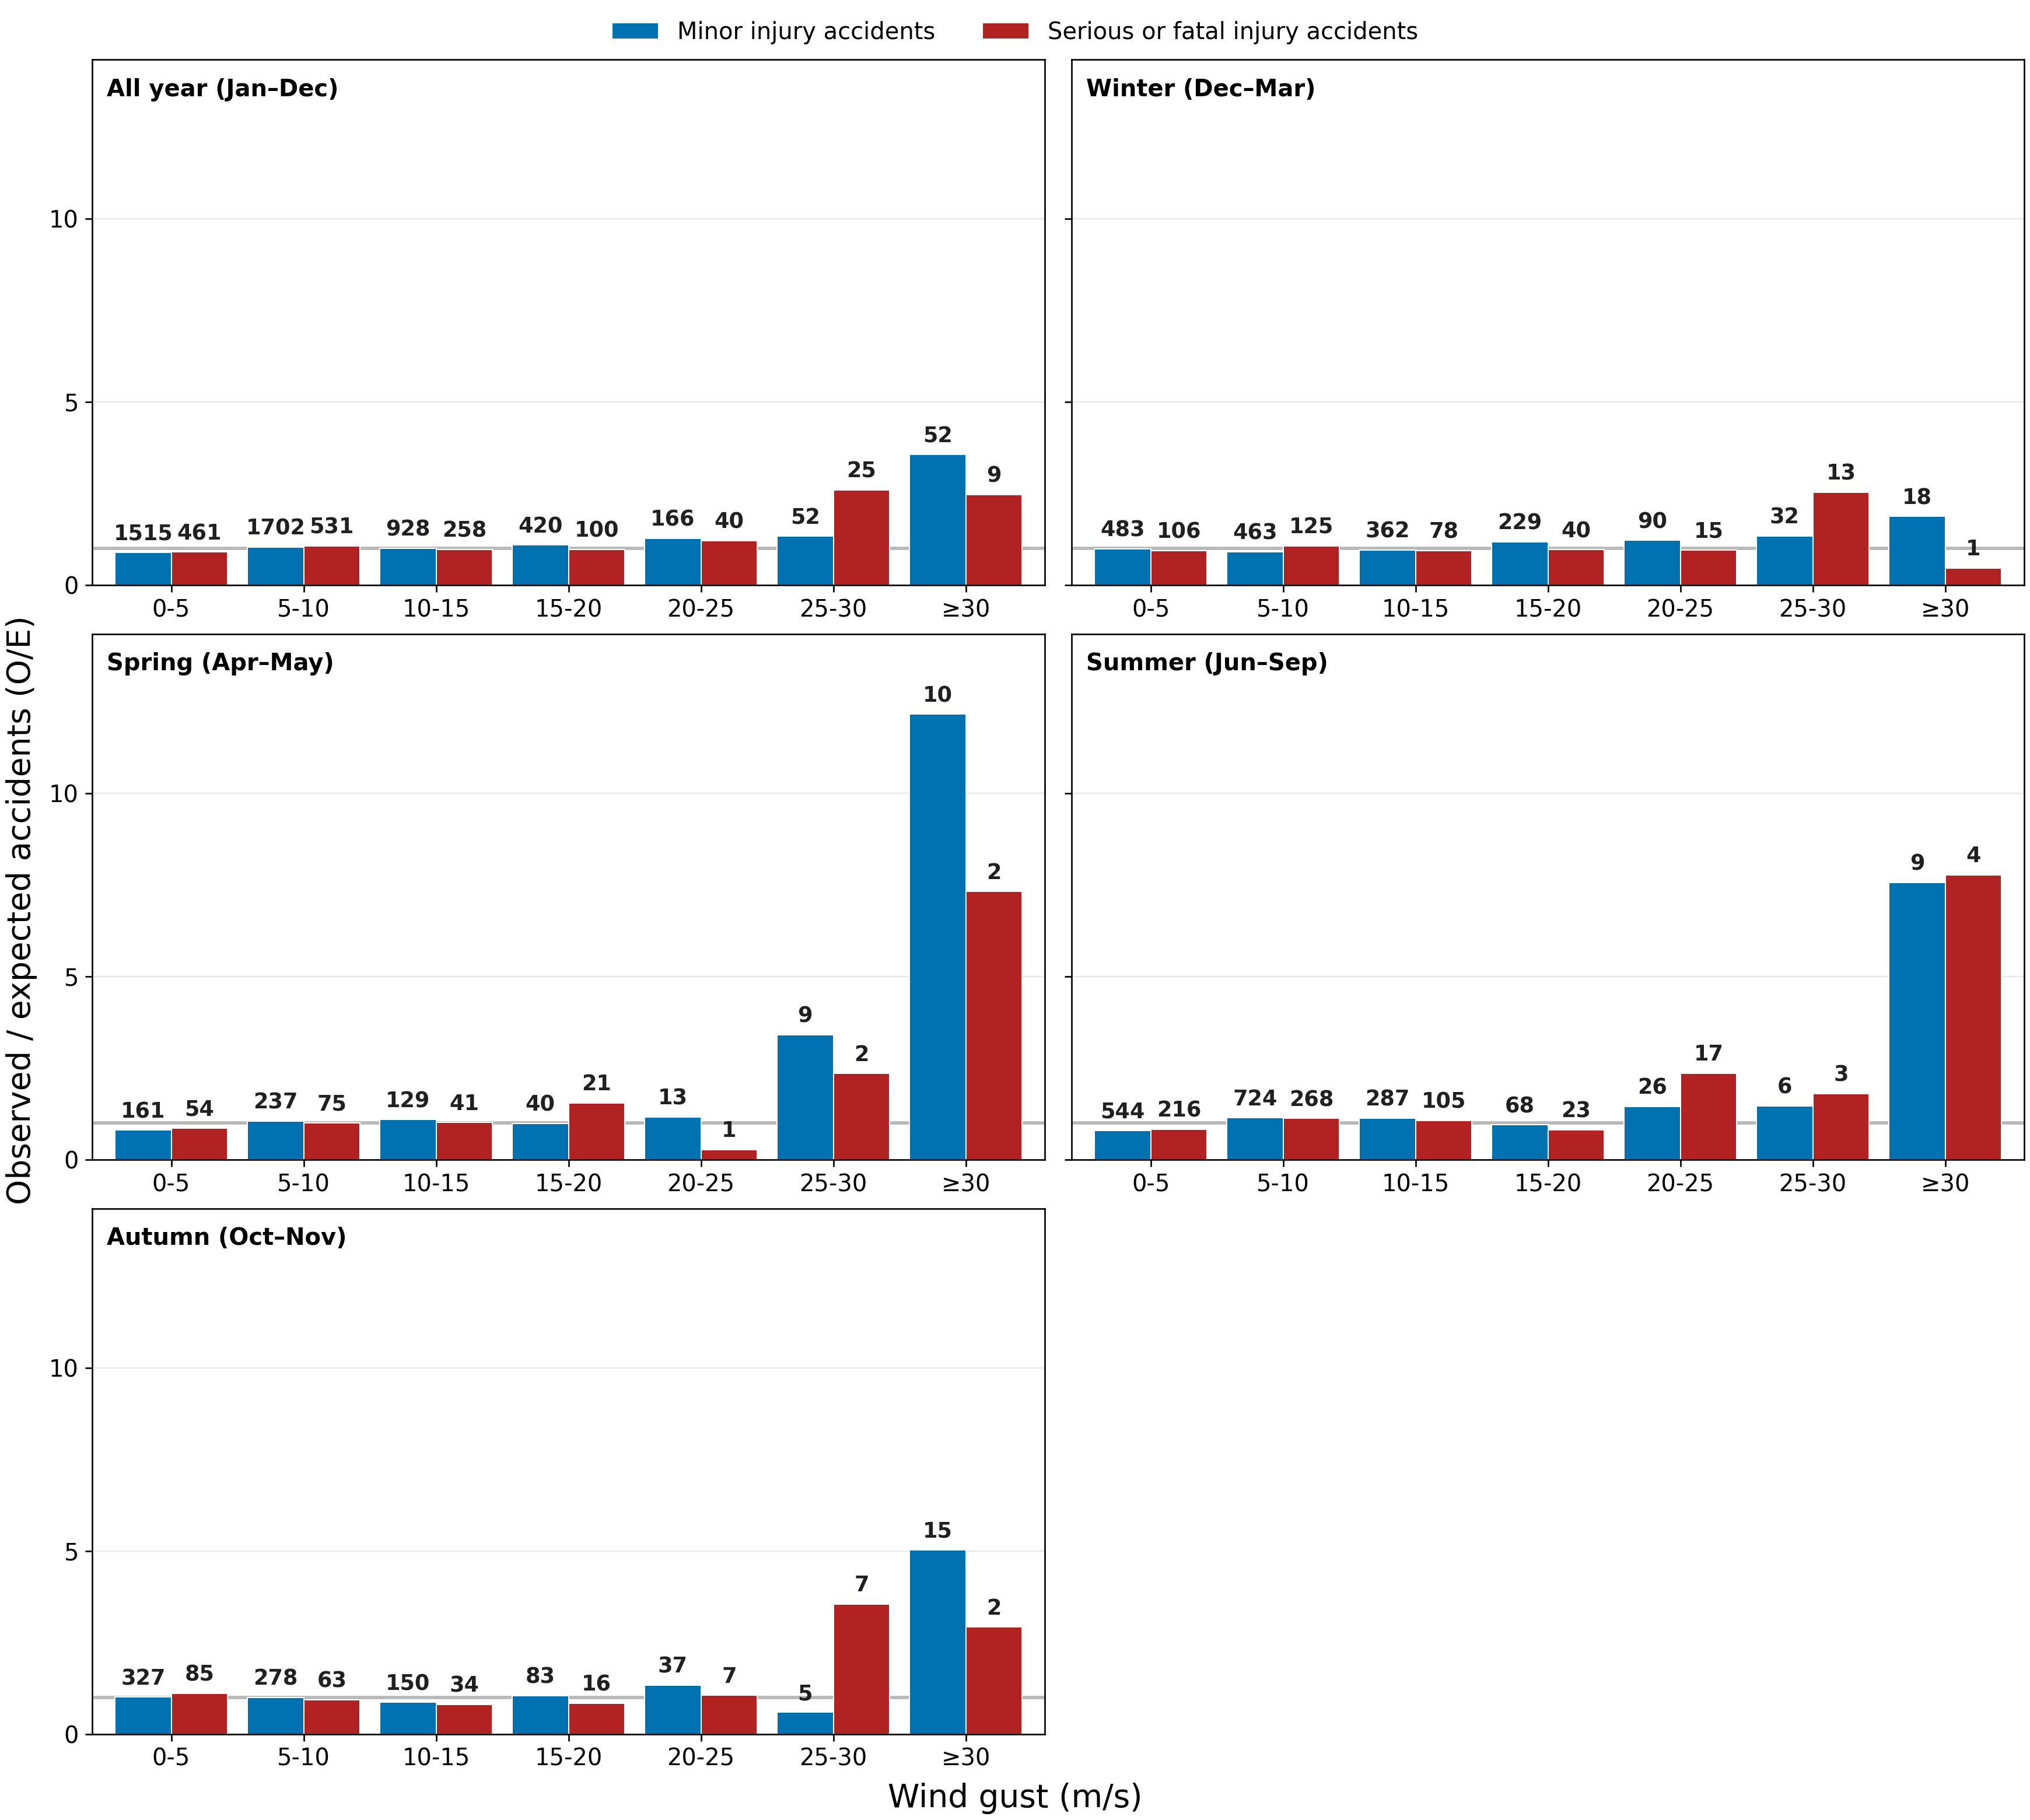
\includegraphics[width=\textwidth,height=0.82\textheight,keepaspectratio]{gust_oe_panels.png}
\caption[All-year and seasonal wind-gust O/E.]{All-year and seasonal wind-gust O/E. Gust is taken from the same
10-minute observation as the accident-time mean wind and is not a daily
maximum. Blue bars show minor injury and red bars show serious or fatal injury;
labels above bars are observed accident counts. The grey reference line is
O/E = 1. Several seasonal upper-gust cells contain few accidents and are
therefore descriptive.}
\label{fig:gust-oe-panels}
\end{figure}

\subsection{Temperature}

Temperature has a non-monotonic pattern in Figure~\ref{fig:temperature-oe-panels}:
O/E is lower at moderate temperatures and higher in some colder and warmer
intervals. Both injury groups show this broad shape, but seasonal extremes
contain few accidents. The finding is secondary and does not establish a
causal temperature effect.

\begin{figure}[!htbp]
\centering
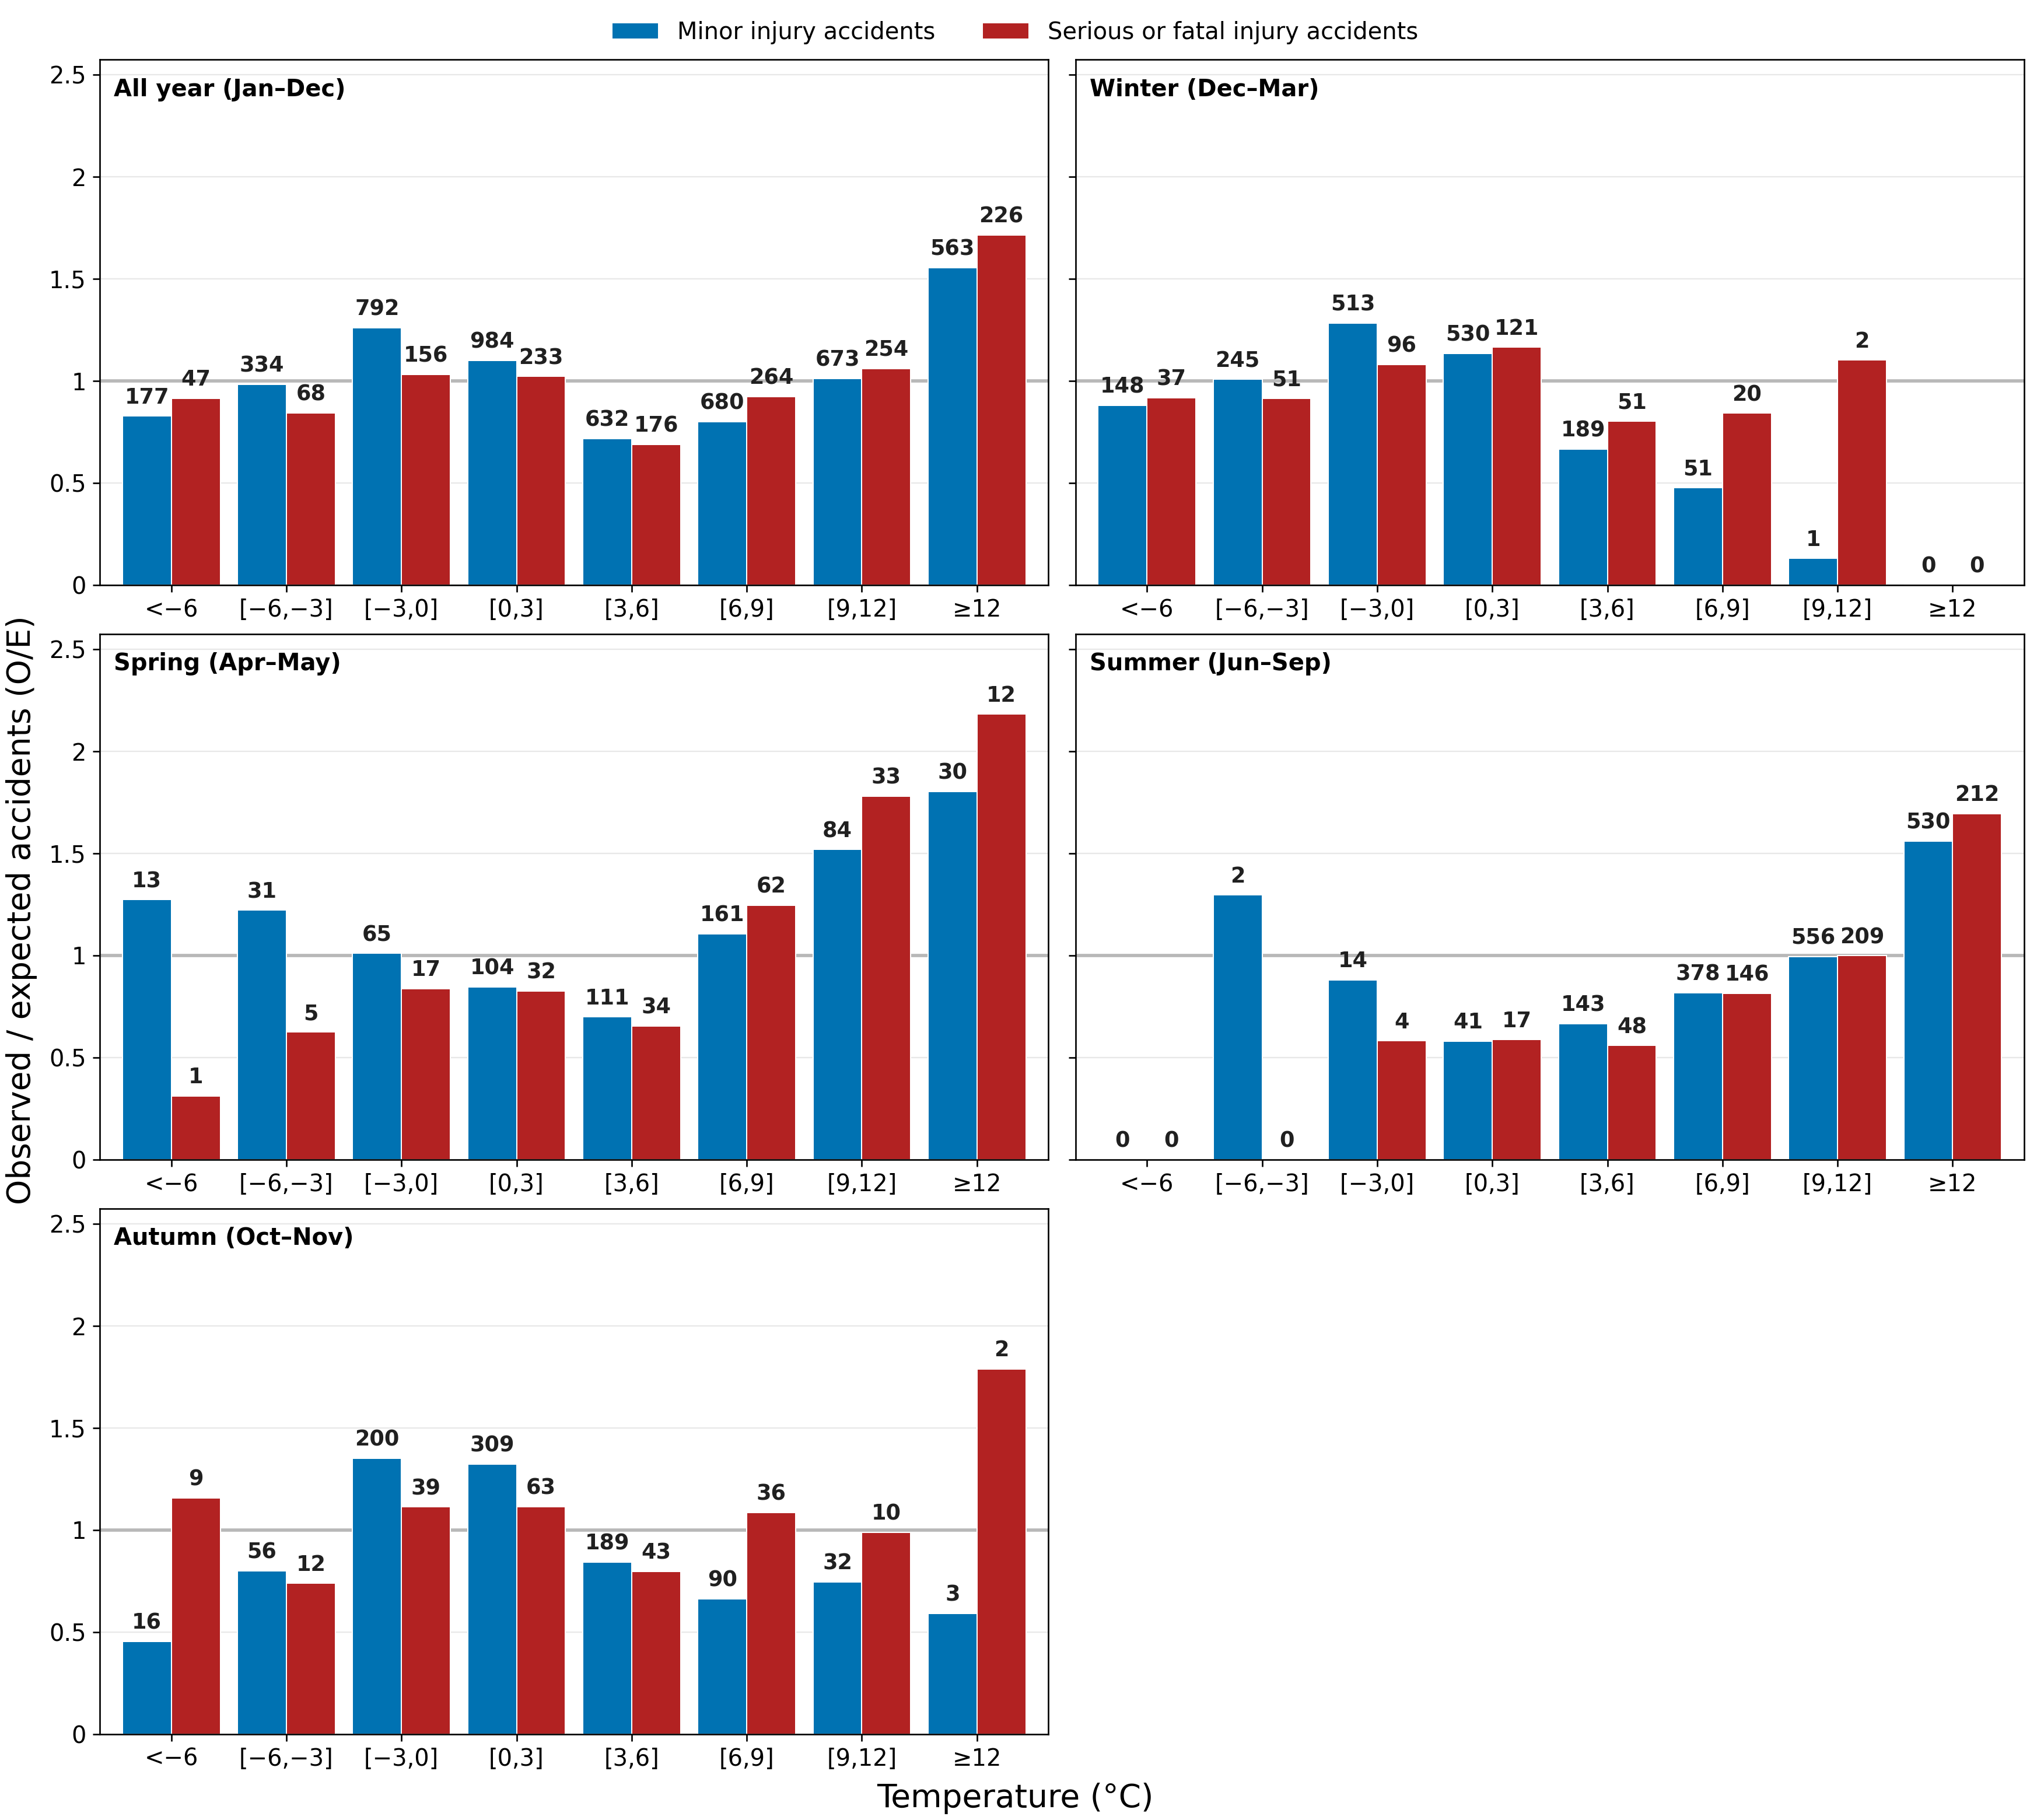
\includegraphics[width=\textwidth,height=0.82\textheight,keepaspectratio]{temperature_oe_panels.png}
\caption[All-year and seasonal temperature O/E.]{All-year and seasonal temperature O/E, standardised within matched
temperature station and study season. Blue bars show minor injury and red bars
show serious or fatal injury; labels above bars are observed accident counts.
The grey reference line is O/E = 1. The non-monotonic pattern and sparse
seasonal extremes are interpreted cautiously.}
\label{fig:temperature-oe-panels}
\end{figure}

Adding year to the station--season standardisation changes the selected O/E
estimates only slightly. The pre-specified comparison is therefore retained
as Q1.

\section{Traffic Response and Approximate O/E Correction}

\subsection{Traffic Behaviour and the Baseline Limitation}

Figure~\ref{fig:traffic-response} shows the traffic response underlying the
correction. Values below 100\% indicate less traffic than the counter's
calendar expectation, not fewer accidents. The upper wind and gust intervals
show reductions. Temperature is included because the existing response output
also estimates that relationship; it does not define a new temperature Q3 rate.

\begin{figure}[p]
\centering
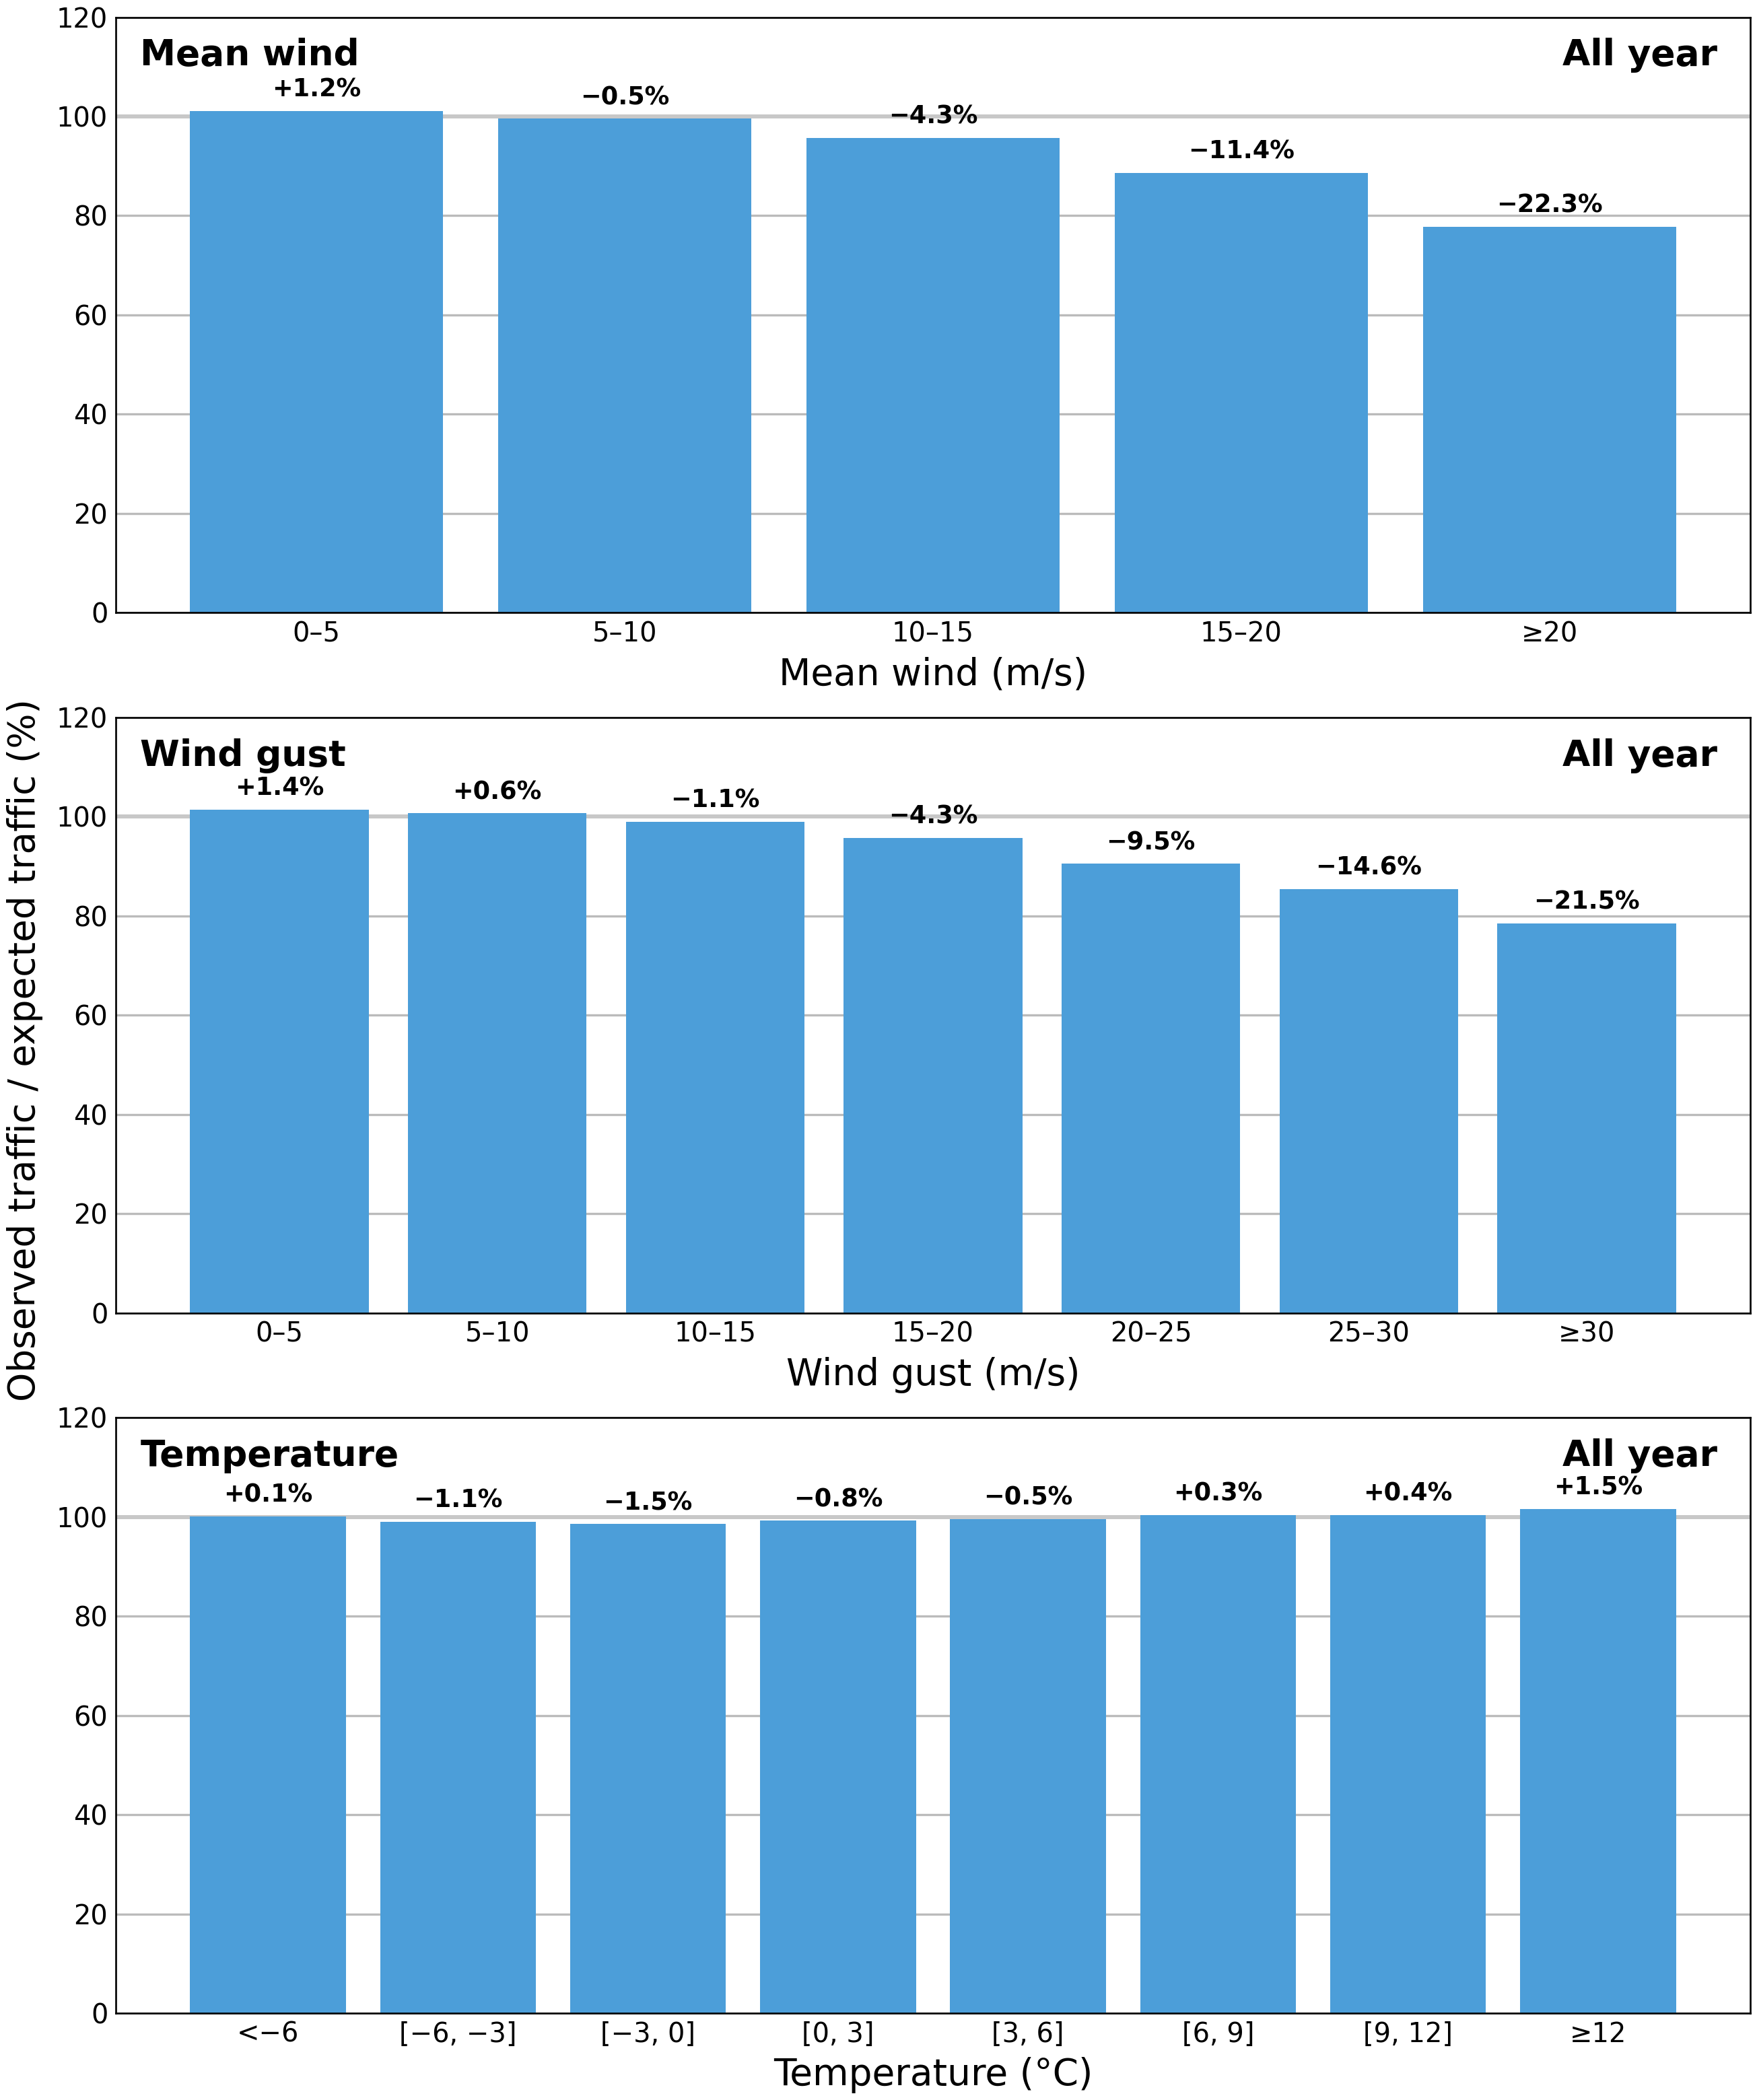
\includegraphics[width=\textwidth,height=0.73\textheight,keepaspectratio]{traffic_weather_response.png}
\caption[Daily traffic relative to calendar expectation.]{Observed daily traffic
relative to expected traffic at counter sections, 2019--2024, pooled across
seasons. The expectation uses the same section, year, month and weekday among
positive-count days. Counts are allocated by observed 07:00--24:00 weather-bin
minutes; bars show the ratio of pooled allocated observed to expected traffic.
The line marks 100\%; labels show percentage changes, not accident counts.}
\label{fig:traffic-response}
\end{figure}

This motivates an approximate correction under the assumption that the traffic response observed at the selected counters is
informative for the wider road network. It does not establish the magnitude of
a national per-vehicle-kilometre contrast, because the traffic response is
estimated over a shorter period and from a geographically selective set of
counters.

\clearpage
\subsection{Full-Period Correction}

The primary O/E uses weather time rather than vehicle exposure. Daily-counter
data from 2019--2024 show that traffic is lower in the strongest wind and gust
intervals, so Q2 applies the estimated counter response to the primary
station--season denominator as a sensitivity analysis. The observed accident
counts remain unchanged; only the expected distribution is reweighted.

The change is visible directly in Figures~\ref{fig:traffic-corrected-wind}
and \ref{fig:traffic-corrected-gust}: upper-bin O/E rises from 2.15 to 2.71
for mean wind and from 3.34 to 4.20 for gust. Outlined bars show Q1 and filled
teal bars show Q2 for the same all-injury population. Thus, accounting for lower
traffic strengthens the high-wind contrast. The validated correction is
available only for All year.

\begin{figure}[H]
\centering
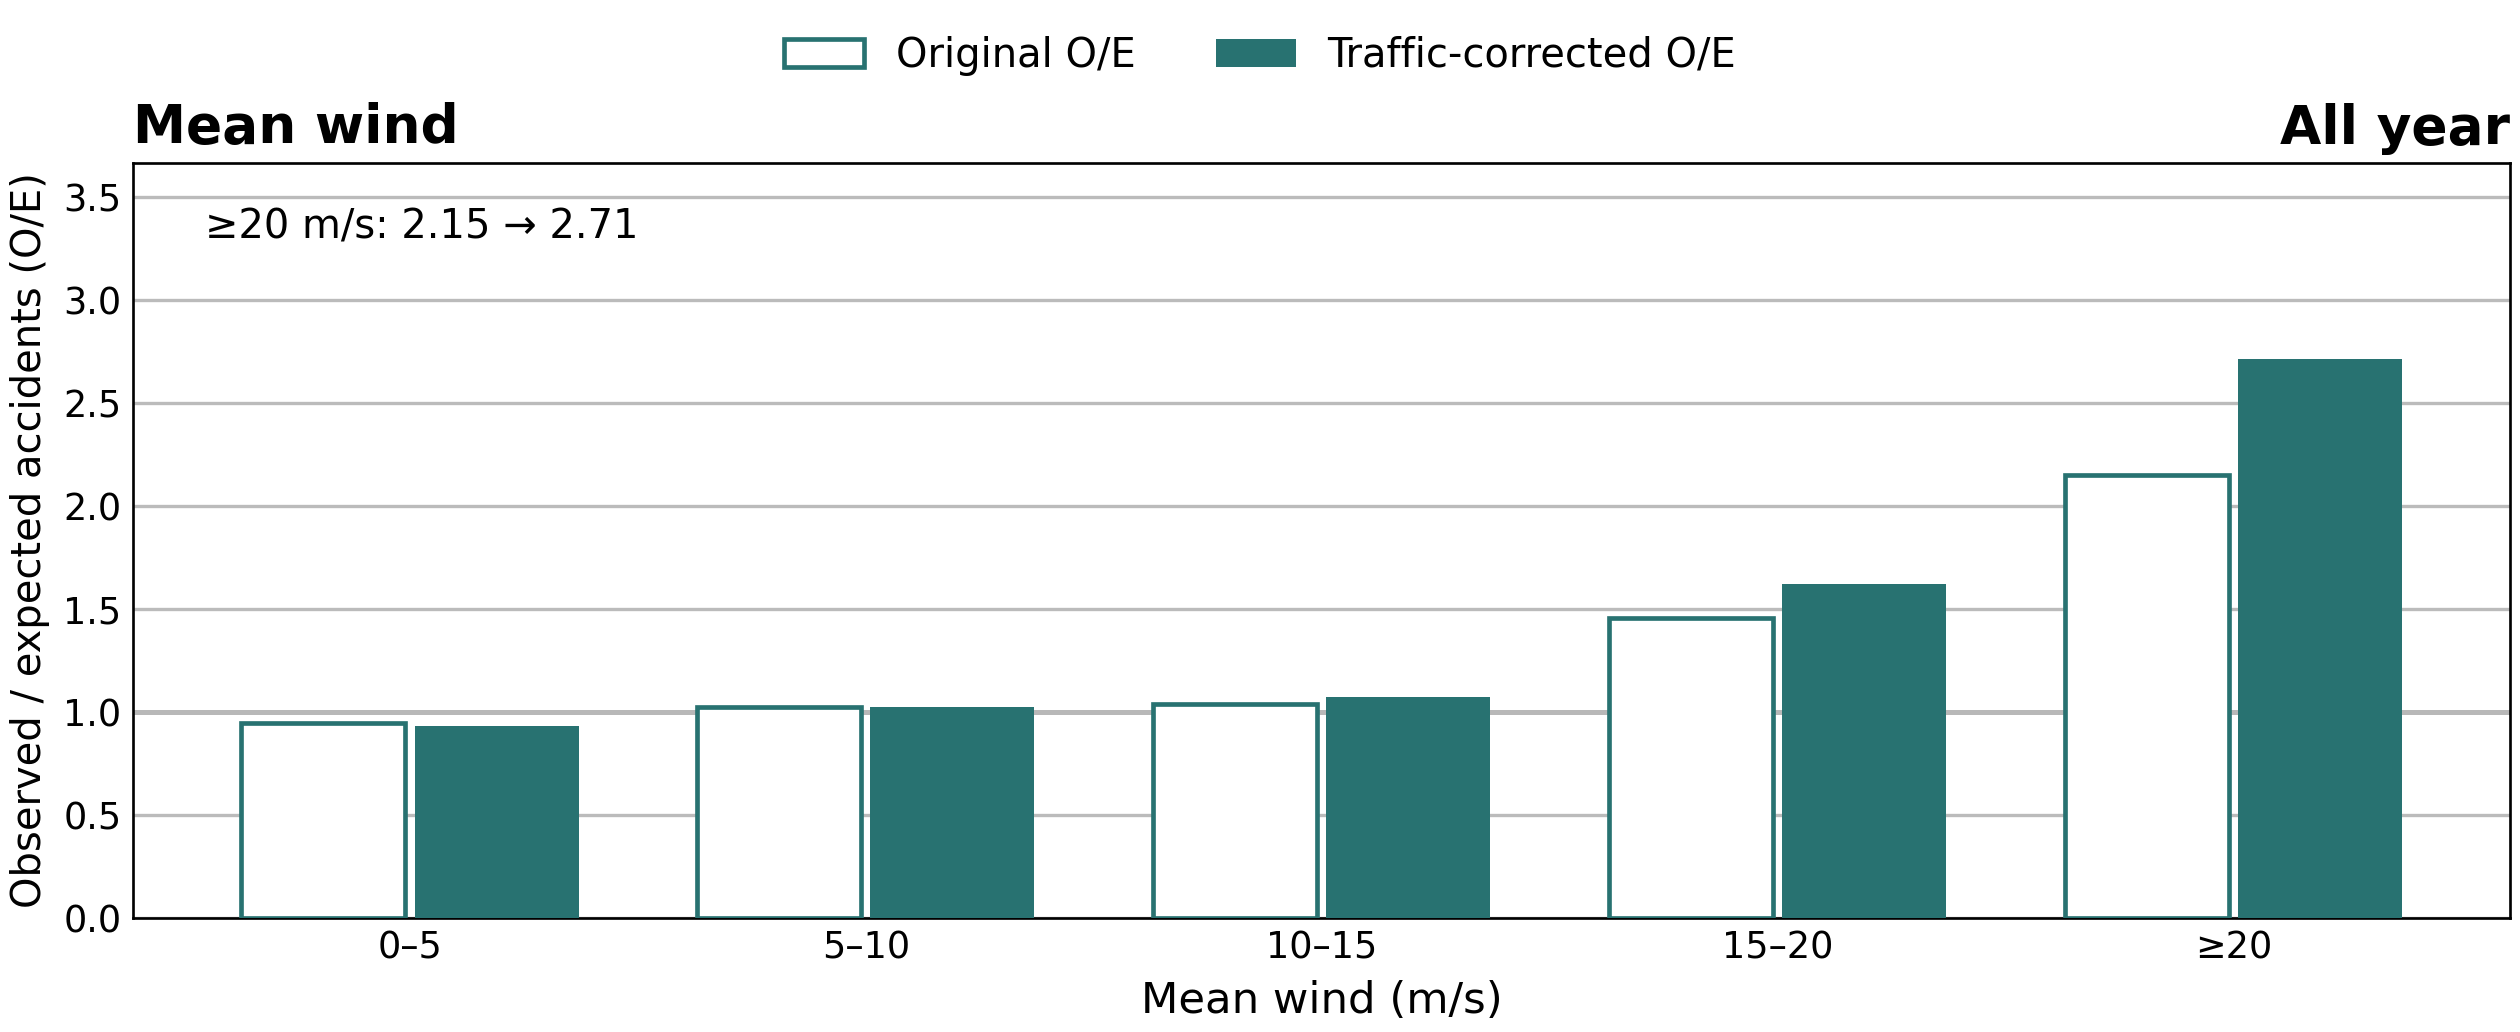
\includegraphics[width=\textwidth]{weather_oe_traffic_corrected_f.png}
\caption[Original and traffic-corrected mean-wind O/E.]{Original and approximately
traffic-corrected mean-wind O/E for all qualifying rural injury accidents,
2007--2025, All year. Outlined bars use weather frequency; teal bars reweight
it using the 2019--2024 counter response. The annotation highlights the upper-bin change; the reference line is O/E = 1. Extrapolation beyond the counters
and absence of hourly traffic make this a model-based sensitivity analysis.}
\label{fig:traffic-corrected-wind}
\end{figure}

\clearpage
\begin{figure}[H]
\centering
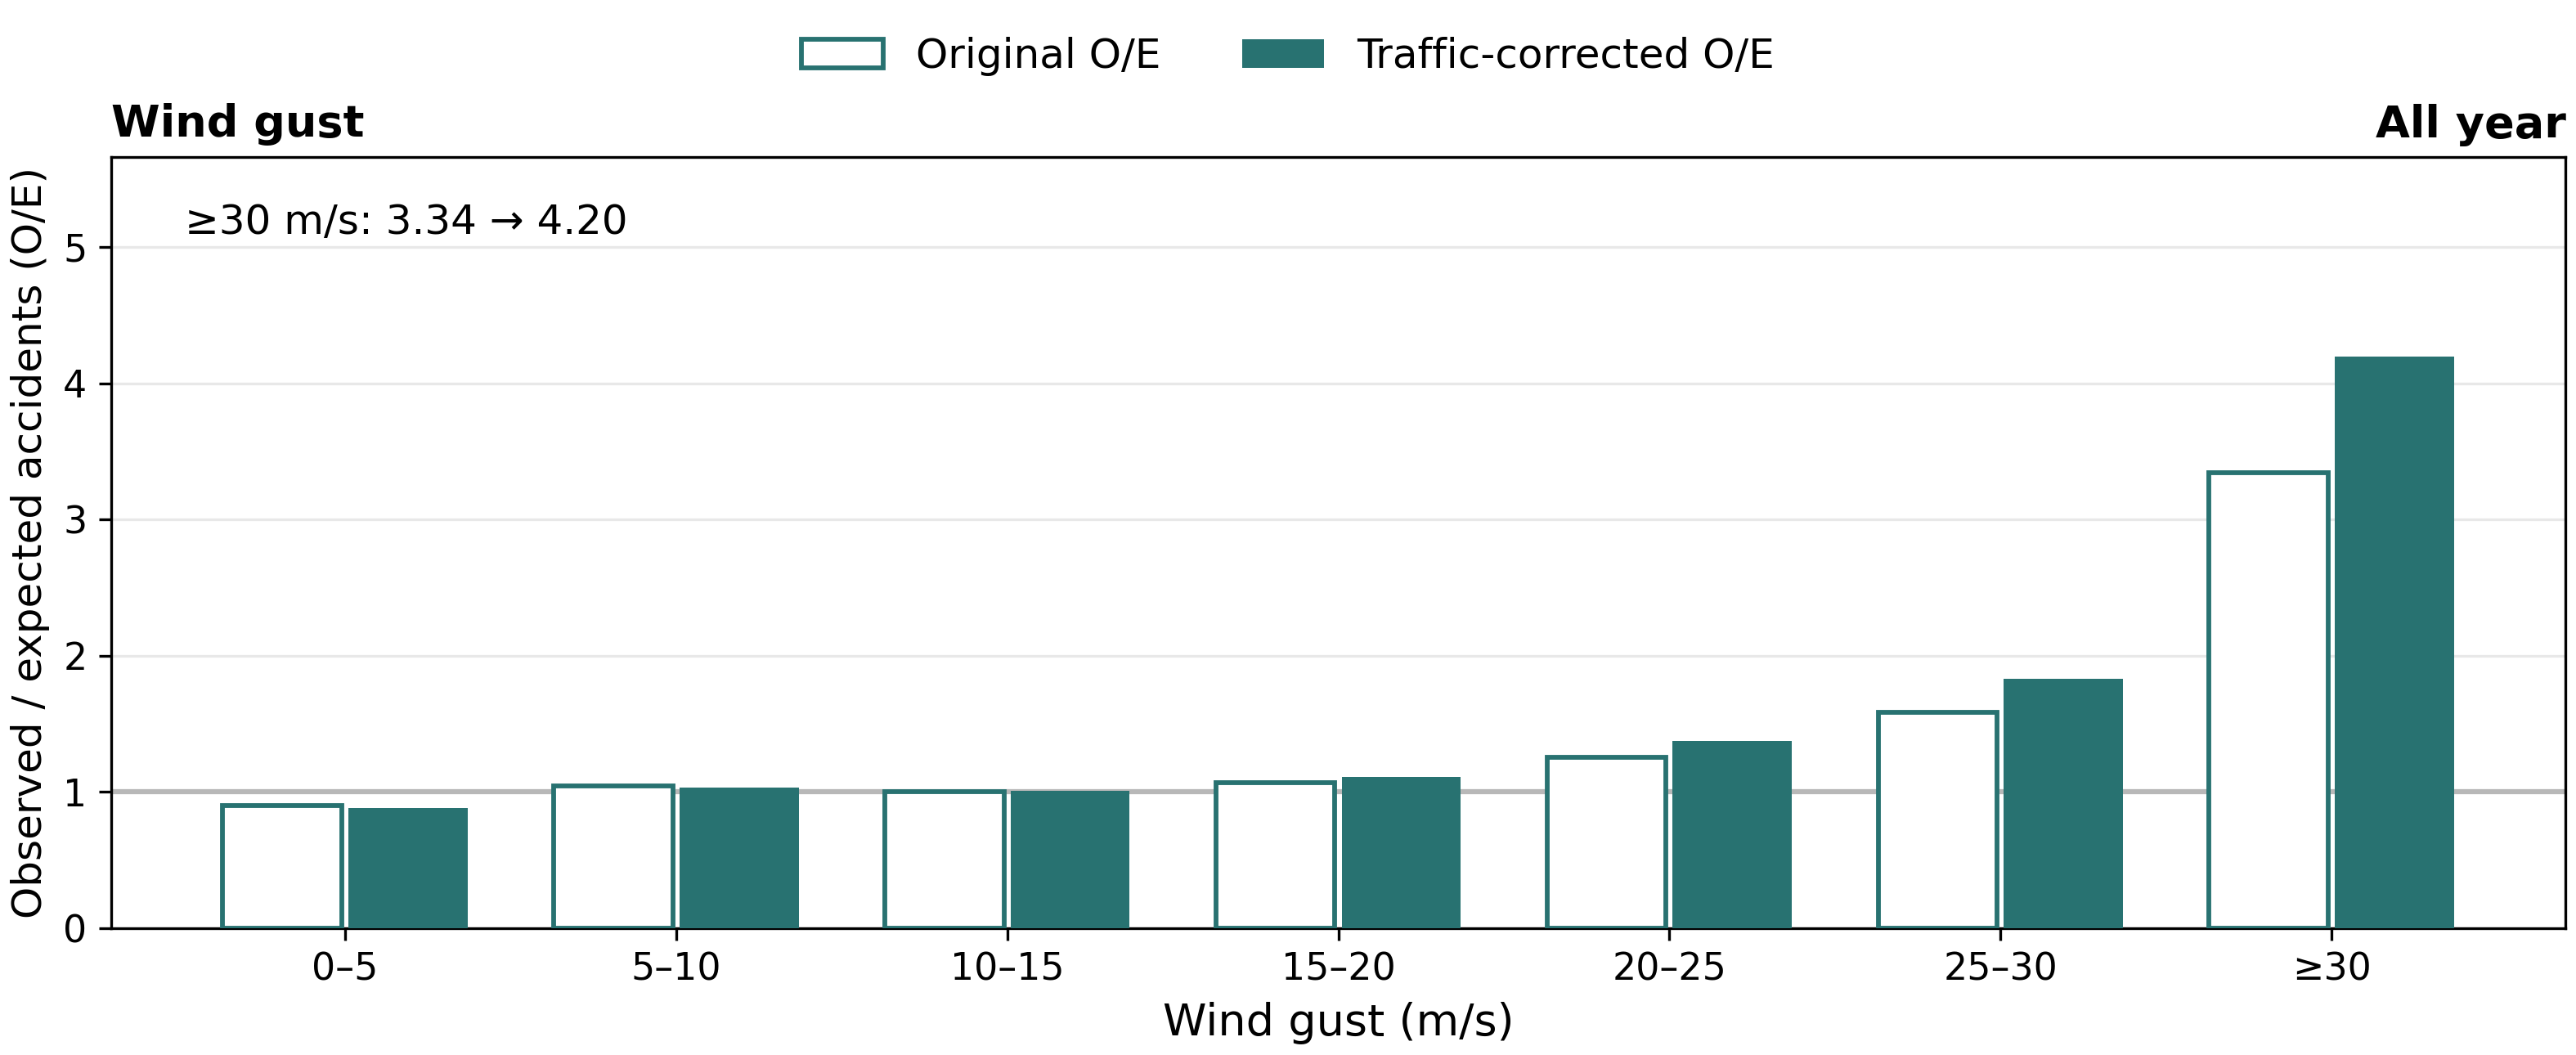
\includegraphics[width=\textwidth]{weather_oe_traffic_corrected_fg.png}
\caption[Original and traffic-corrected wind-gust O/E.]{Original and approximately
traffic-corrected wind-gust O/E for all qualifying rural injury accidents,
2007--2025, All year. Outlined and teal bars use the original and reweighted
expected counts, respectively. The annotation highlights the upper-bin change;
the reference line is O/E = 1. The 2019--2024 daily-counter response is extrapolated to the
wider population and does not identify hourly traffic exposure.}
\label{fig:traffic-corrected-gust}
\end{figure}

Figure~\ref{fig:corrected-injury-groups} retains the corrected comparison
separately for minor injury and serious or fatal injury, matching Q1's two
groups. This shows whether the corrected upper-wind pattern is shared across
injury categories. Differences between the bars are not a test of severity,
particularly where the serious or fatal counts are small.

\begin{figure}[p]
\centering
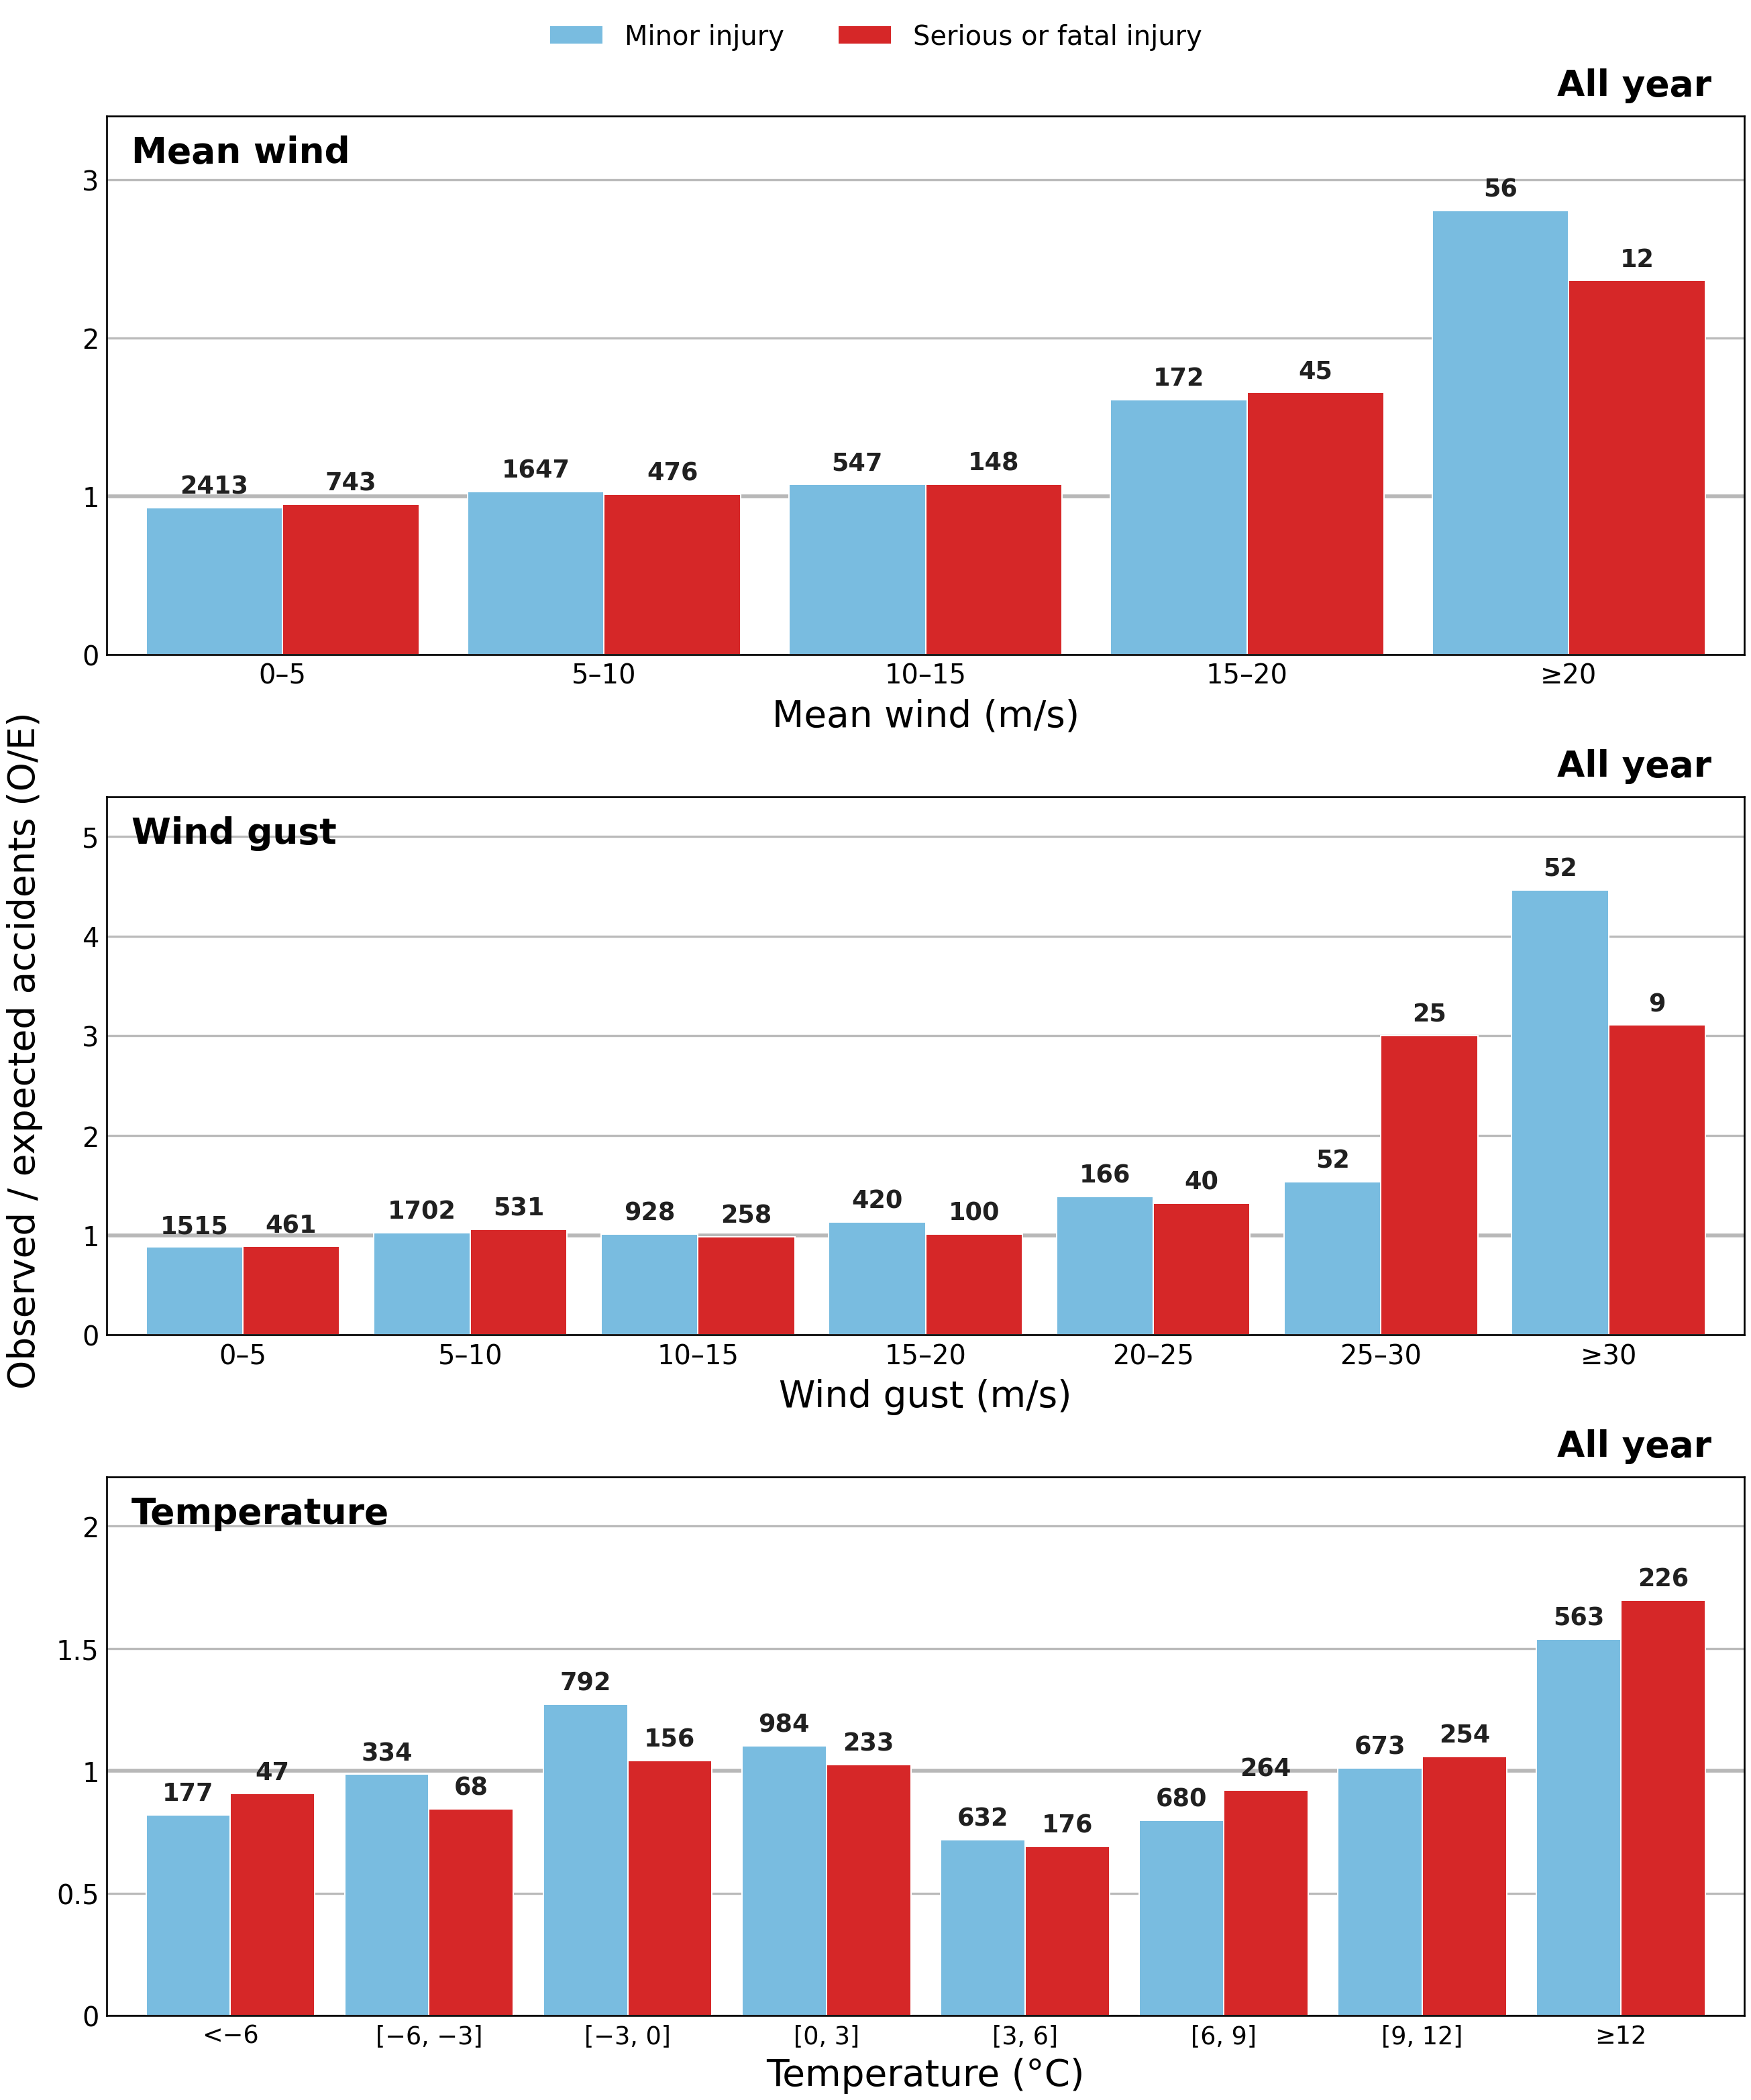
\includegraphics[width=\textwidth,height=0.73\textheight,keepaspectratio]{weather_oe_traffic_corrected.png}
\caption[Traffic-corrected O/E by injury group.]{Approximately traffic-corrected
mean-wind and gust O/E, 2007--2025, All year. Blue and red bars represent
minor injury and serious or fatal injury. Each group's expected count is
reweighted using the 2019--2024 counter response; labels give observed counts.
The line marks O/E = 1. These disjoint groups complement the all-injury
original--corrected comparison; the same extrapolation and hourly-traffic
limitations apply.}
\label{fig:corrected-injury-groups}
\end{figure}

\clearpage
\subsection{Period Comparison and Counter-Era Correction}

Figures~\ref{fig:oe-early-period} and \ref{fig:oe-counter-period} show the
period comparison for mean wind, gust and temperature.
Each figure pools accidents and background weather over its stated years.
These are All year comparisons for different periods, not seasonal estimates
or replacements for the full-period Q1 figures. Upper-bin counts should be read
alongside the bar heights when comparing the periods.

\begin{figure}[p]
\centering
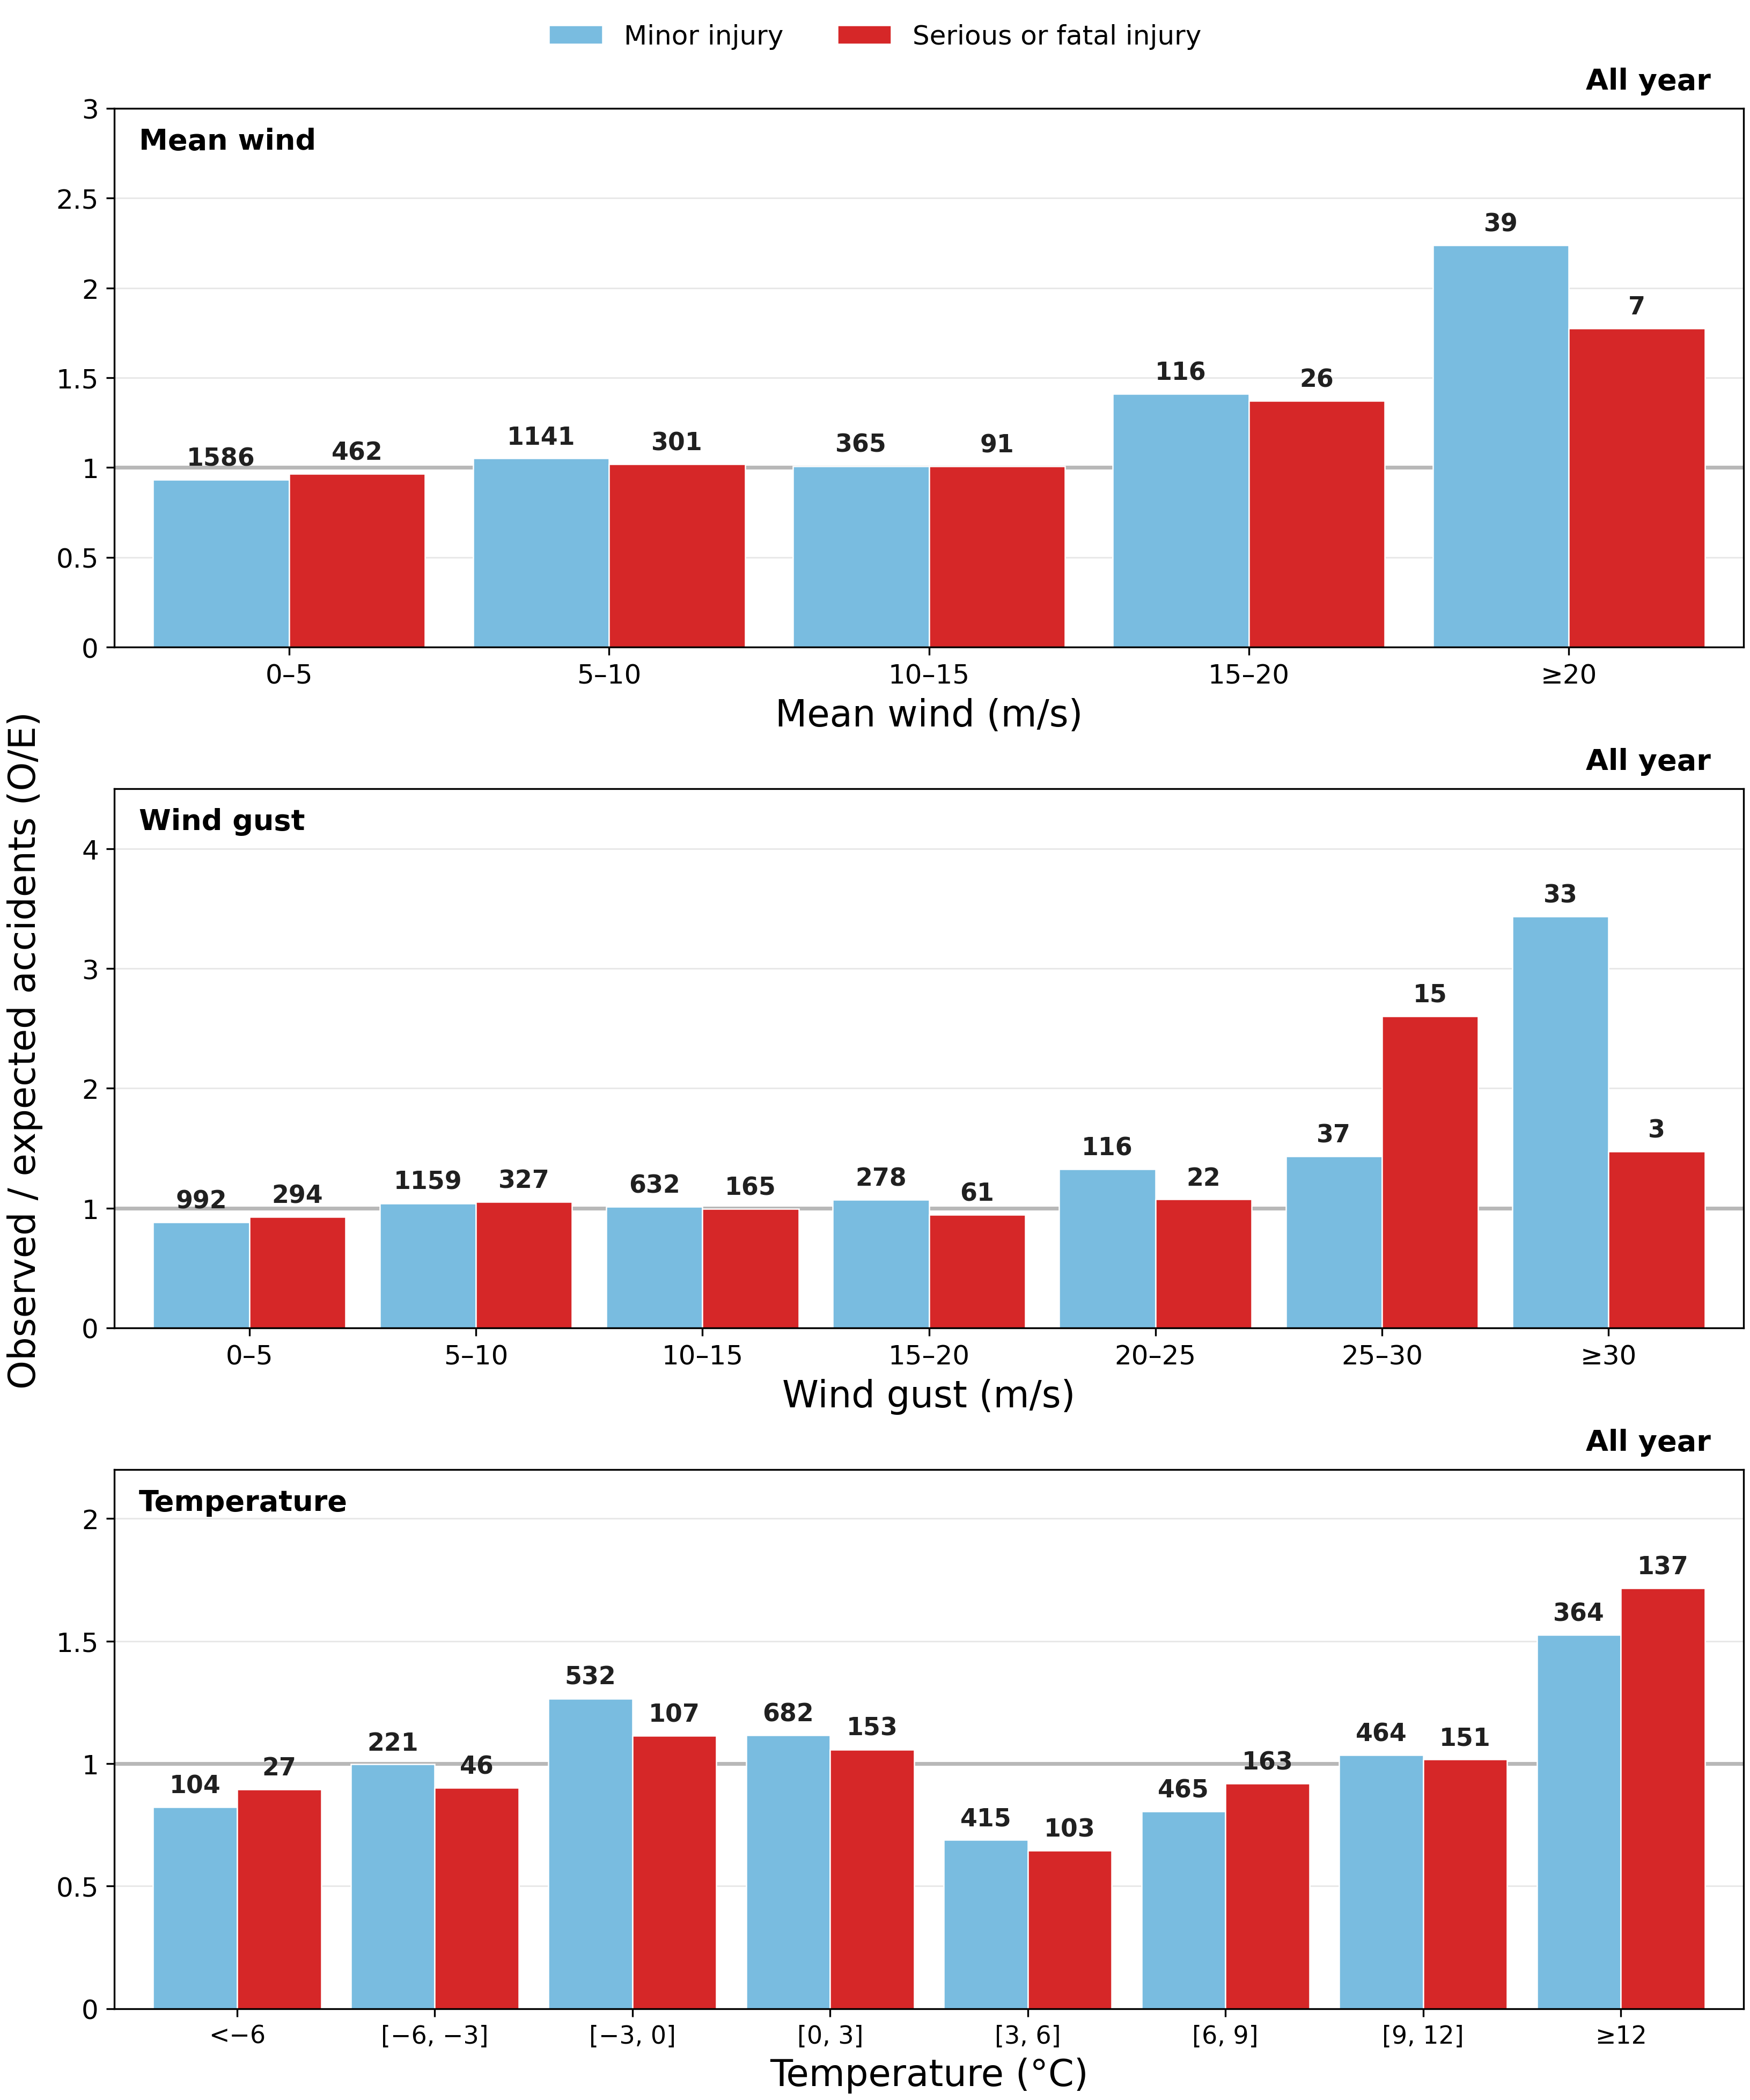
\includegraphics[width=\textwidth,height=0.73\textheight,keepaspectratio]{weather_oe_2007_2018.png}
\caption[All year weather-frequency O/E, 2007--2018.]{Period comparison: All year weather-frequency
O/E for rural injury accidents in 2007--2018. Accident counts and station--season
background weather are restricted to the same years. Blue and red bars show
minor injury and serious or fatal injury separately; labels are accident counts.
The line marks O/E = 1. This period-specific comparison contains no traffic
adjustment and should be interpreted with its sparse upper bins.}
\label{fig:oe-early-period}
\end{figure}

\begin{figure}[p]
\centering
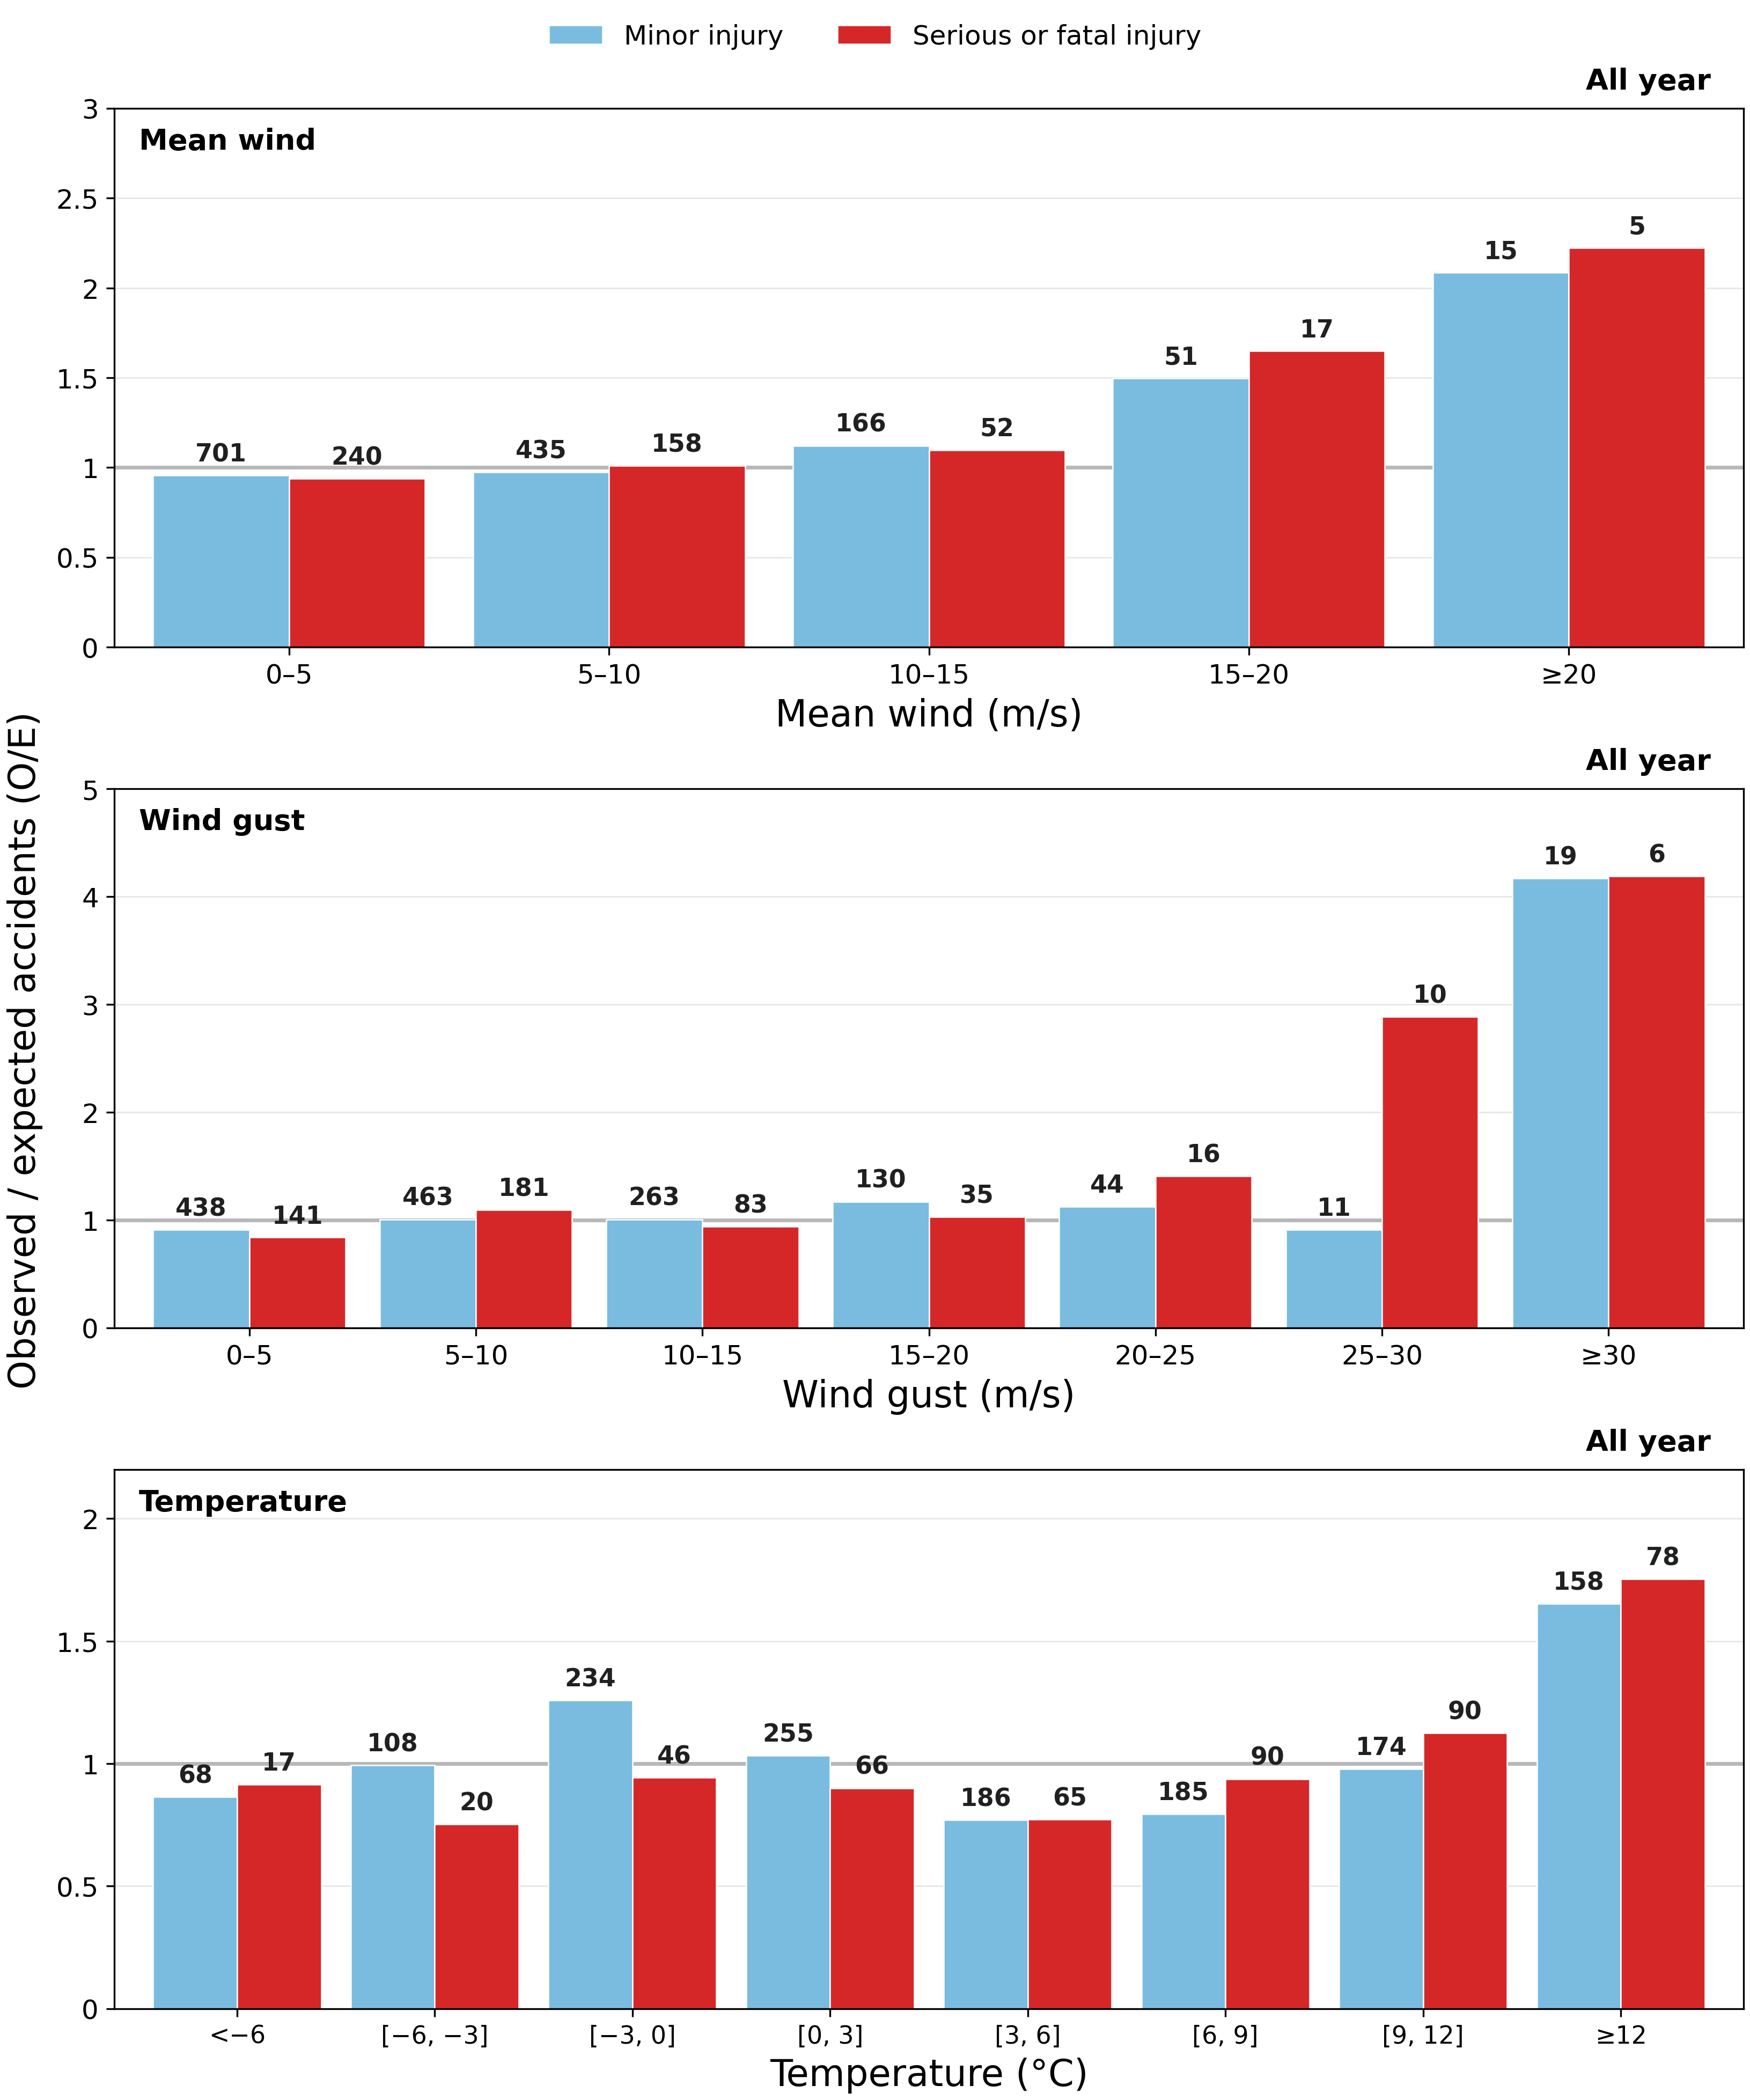
\includegraphics[width=\textwidth,height=0.73\textheight,keepaspectratio]{weather_oe_2019_2024.png}
\caption[All year weather-frequency O/E, 2019--2024.]{Period comparison: All year weather-frequency
O/E for rural injury accidents in 2019--2024. Accident counts and station--season
background weather are restricted to the same years. Blue and red bars show
minor injury and serious or fatal injury separately; labels are accident counts.
The line marks O/E = 1. This period-specific comparison contains no traffic
adjustment and should be interpreted with its sparse upper bins.}
\label{fig:oe-counter-period}
\end{figure}

Figure~\ref{fig:corrected-counter-period} shows the existing correction restricted
to 2019--2024, including its temperature result. Its minor-injury and serious or fatal bars can be compared with
Figure~\ref{fig:oe-counter-period}, which uses the same population without
traffic reweighting. This sensitivity output
uses the shorter period's weather background; it must not be substituted for
Q2's full-period estimates. Its temperature panel concerns
corrected weather-frequency O/E, not the Q3 traffic-based rate method.

\begin{figure}[p]
\centering
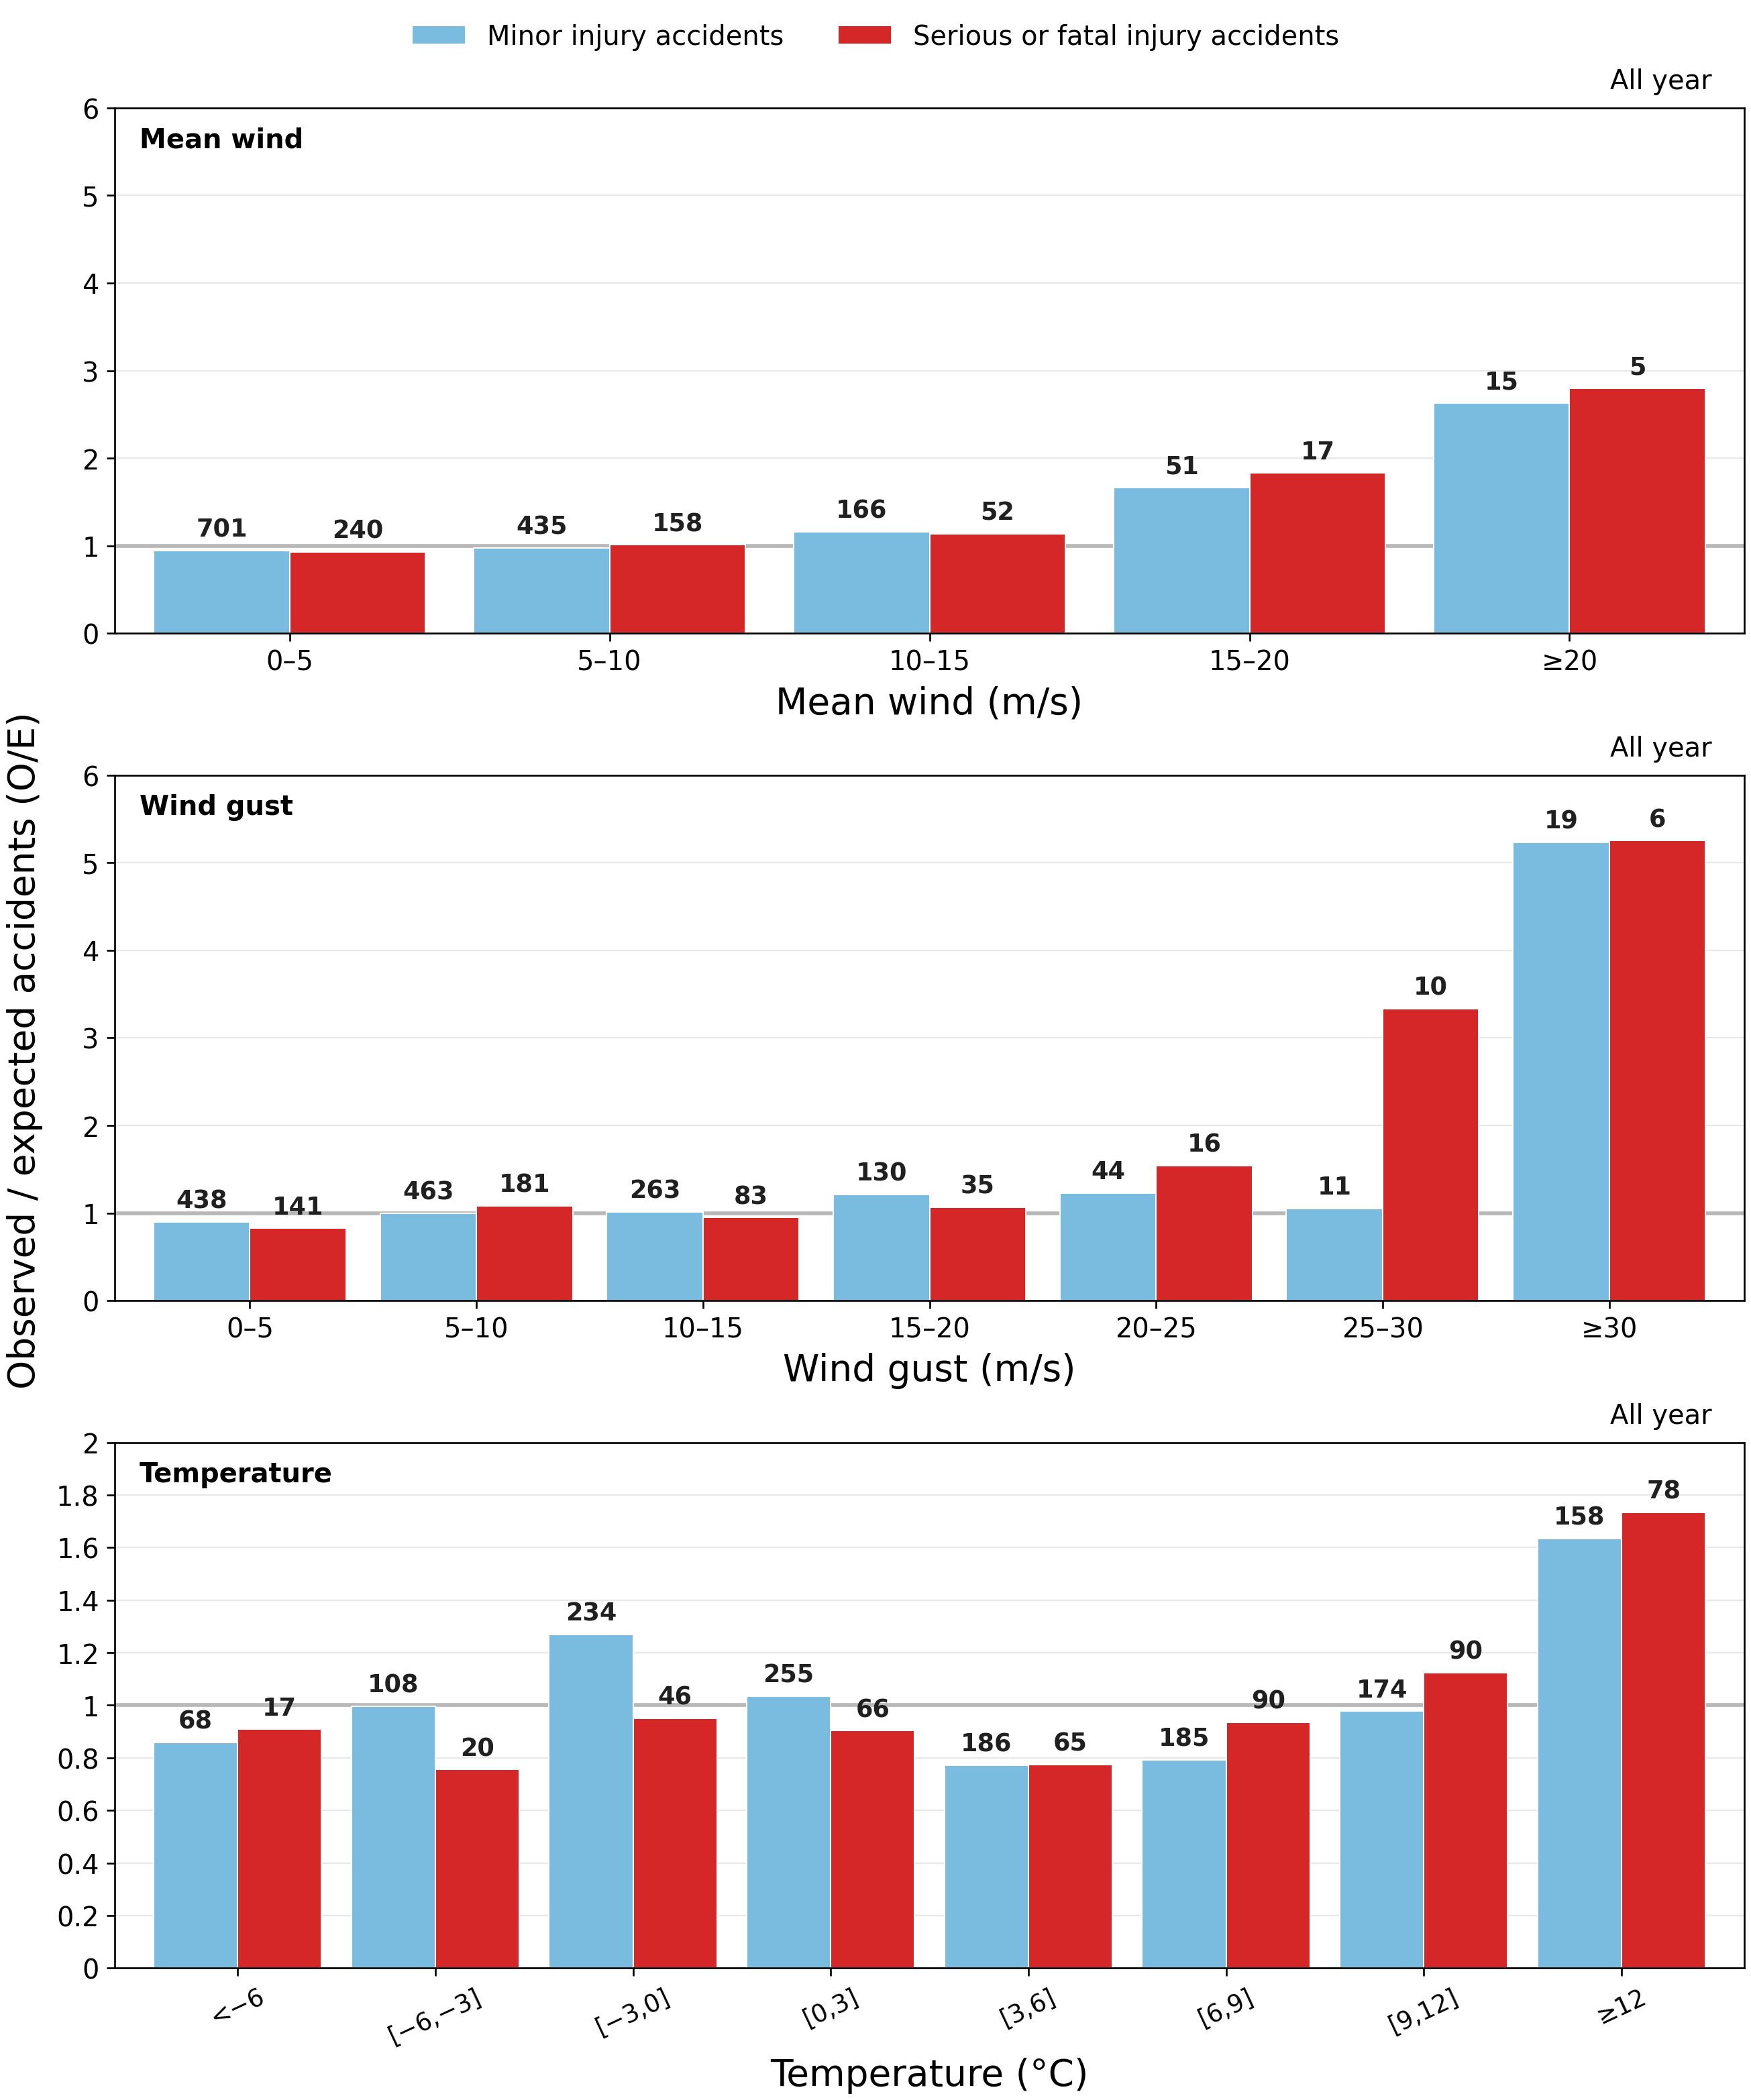
\includegraphics[width=\textwidth,height=0.73\textheight,keepaspectratio]{weather_oe_traffic_corrected_2019_2024.png}
\caption[Traffic-corrected All year O/E by injury group, 2019--2024.]{Approximately
traffic-corrected O/E for qualifying rural injury accidents, 2019--2024,
All year. Blue and red bars show minor injury and serious or fatal injury
using reweighted expected counts within that period. Labels give observed
accidents; the line marks O/E = 1. The daily-counter response includes mean wind, gust and temperature,
but hourly traffic is still unobserved. This is the correction within the counter era.}
\label{fig:corrected-counter-period}
\end{figure}
\clearpage
\section{Counter-Based Accident Rates}

The third stage estimates accident rates in the smaller sample linked to daily
traffic counters. It includes 694 accidents, 533,649 eligible counter-section
days and approximately 5.63 billion estimated vehicle-kilometres.
Table~\ref{tab:monthly-vkt-rate} gives the accident counts, exposure and rates
for each wind interval. The main method uses monthly weather frequencies;
the same-day allocation sensitivity in the following section tests that choice.
Both constructions are defined in the Q3 Methods.

\begin{table}[H]
\centering
\caption[VKT wind and gust counts, exposure and rates.]{VKT wind and gust rates, 2019--2024. Exposure is the full observed daily traffic count times rural section length, allocated by the assigned station's pooled 2007--2025 calendar-month weather frequency for 07:00--24:00.}
\label{tab:monthly-vkt-rate}
\small
\begin{tabular}{llrrr}
\toprule
Measure & Interval (m/s) & Observed & \shortstack{Million estimated\\vehicle-km} & \shortstack{Accidents per million\\estimated vehicle-km} \\ \midrule
Mean wind & 0--5 & 344 & 3011.5 & 0.114 \\ \grayhline
Mean wind & 5--10 & 210 & 1963.5 & 0.107 \\ \grayhline
Mean wind & 10--15 & 96 & 539.9 & 0.178 \\ \grayhline
Mean wind & 15--20 & 33 & 98.9 & 0.334 \\ \grayhline
Mean wind & $\geq$20 & 11 & 16.5 & 0.667 \\ \grayhline
Wind gust & 0--5 & 205 & 1840.9 & 0.111 \\ \grayhline
Wind gust & 5--10 & 238 & 2133.5 & 0.112 \\ \grayhline
Wind gust & 10--15 & 129 & 1085.1 & 0.119 \\ \grayhline
Wind gust & 15--20 & 70 & 400.3 & 0.175 \\ \grayhline
Wind gust & 20--25 & 29 & 123.3 & 0.235 \\ \grayhline
Wind gust & 25--30 & 12 & 34.5 & 0.348 \\ \grayhline
Wind gust & $\geq$30 & 11 & 12.7 & 0.866 \\ \grayhline
\bottomrule
\end{tabular}
\end{table}


Rates rise markedly in the upper wind intervals. At mean wind of at least
20 m/s, the rate is 5.83 times the 0--5 m/s rate; for gusts of at least
30 m/s, the contrast is 7.78. Only 11 accidents contribute to each upper interval, so
these large differences are imprecise. The selective counter coverage also
limits their generalisability.

\subsection{All Year Rates}

Figure~\ref{fig:monthly-vkt-annual} shows the pooled wind and gust rates.
The light-blue and red components share estimated exposure, so their stack
height is the all-injury rate. Counts identify how many accidents contribute;
the bars are not a formal comparison of injury severity.

\begin{figure}[p]
\centering
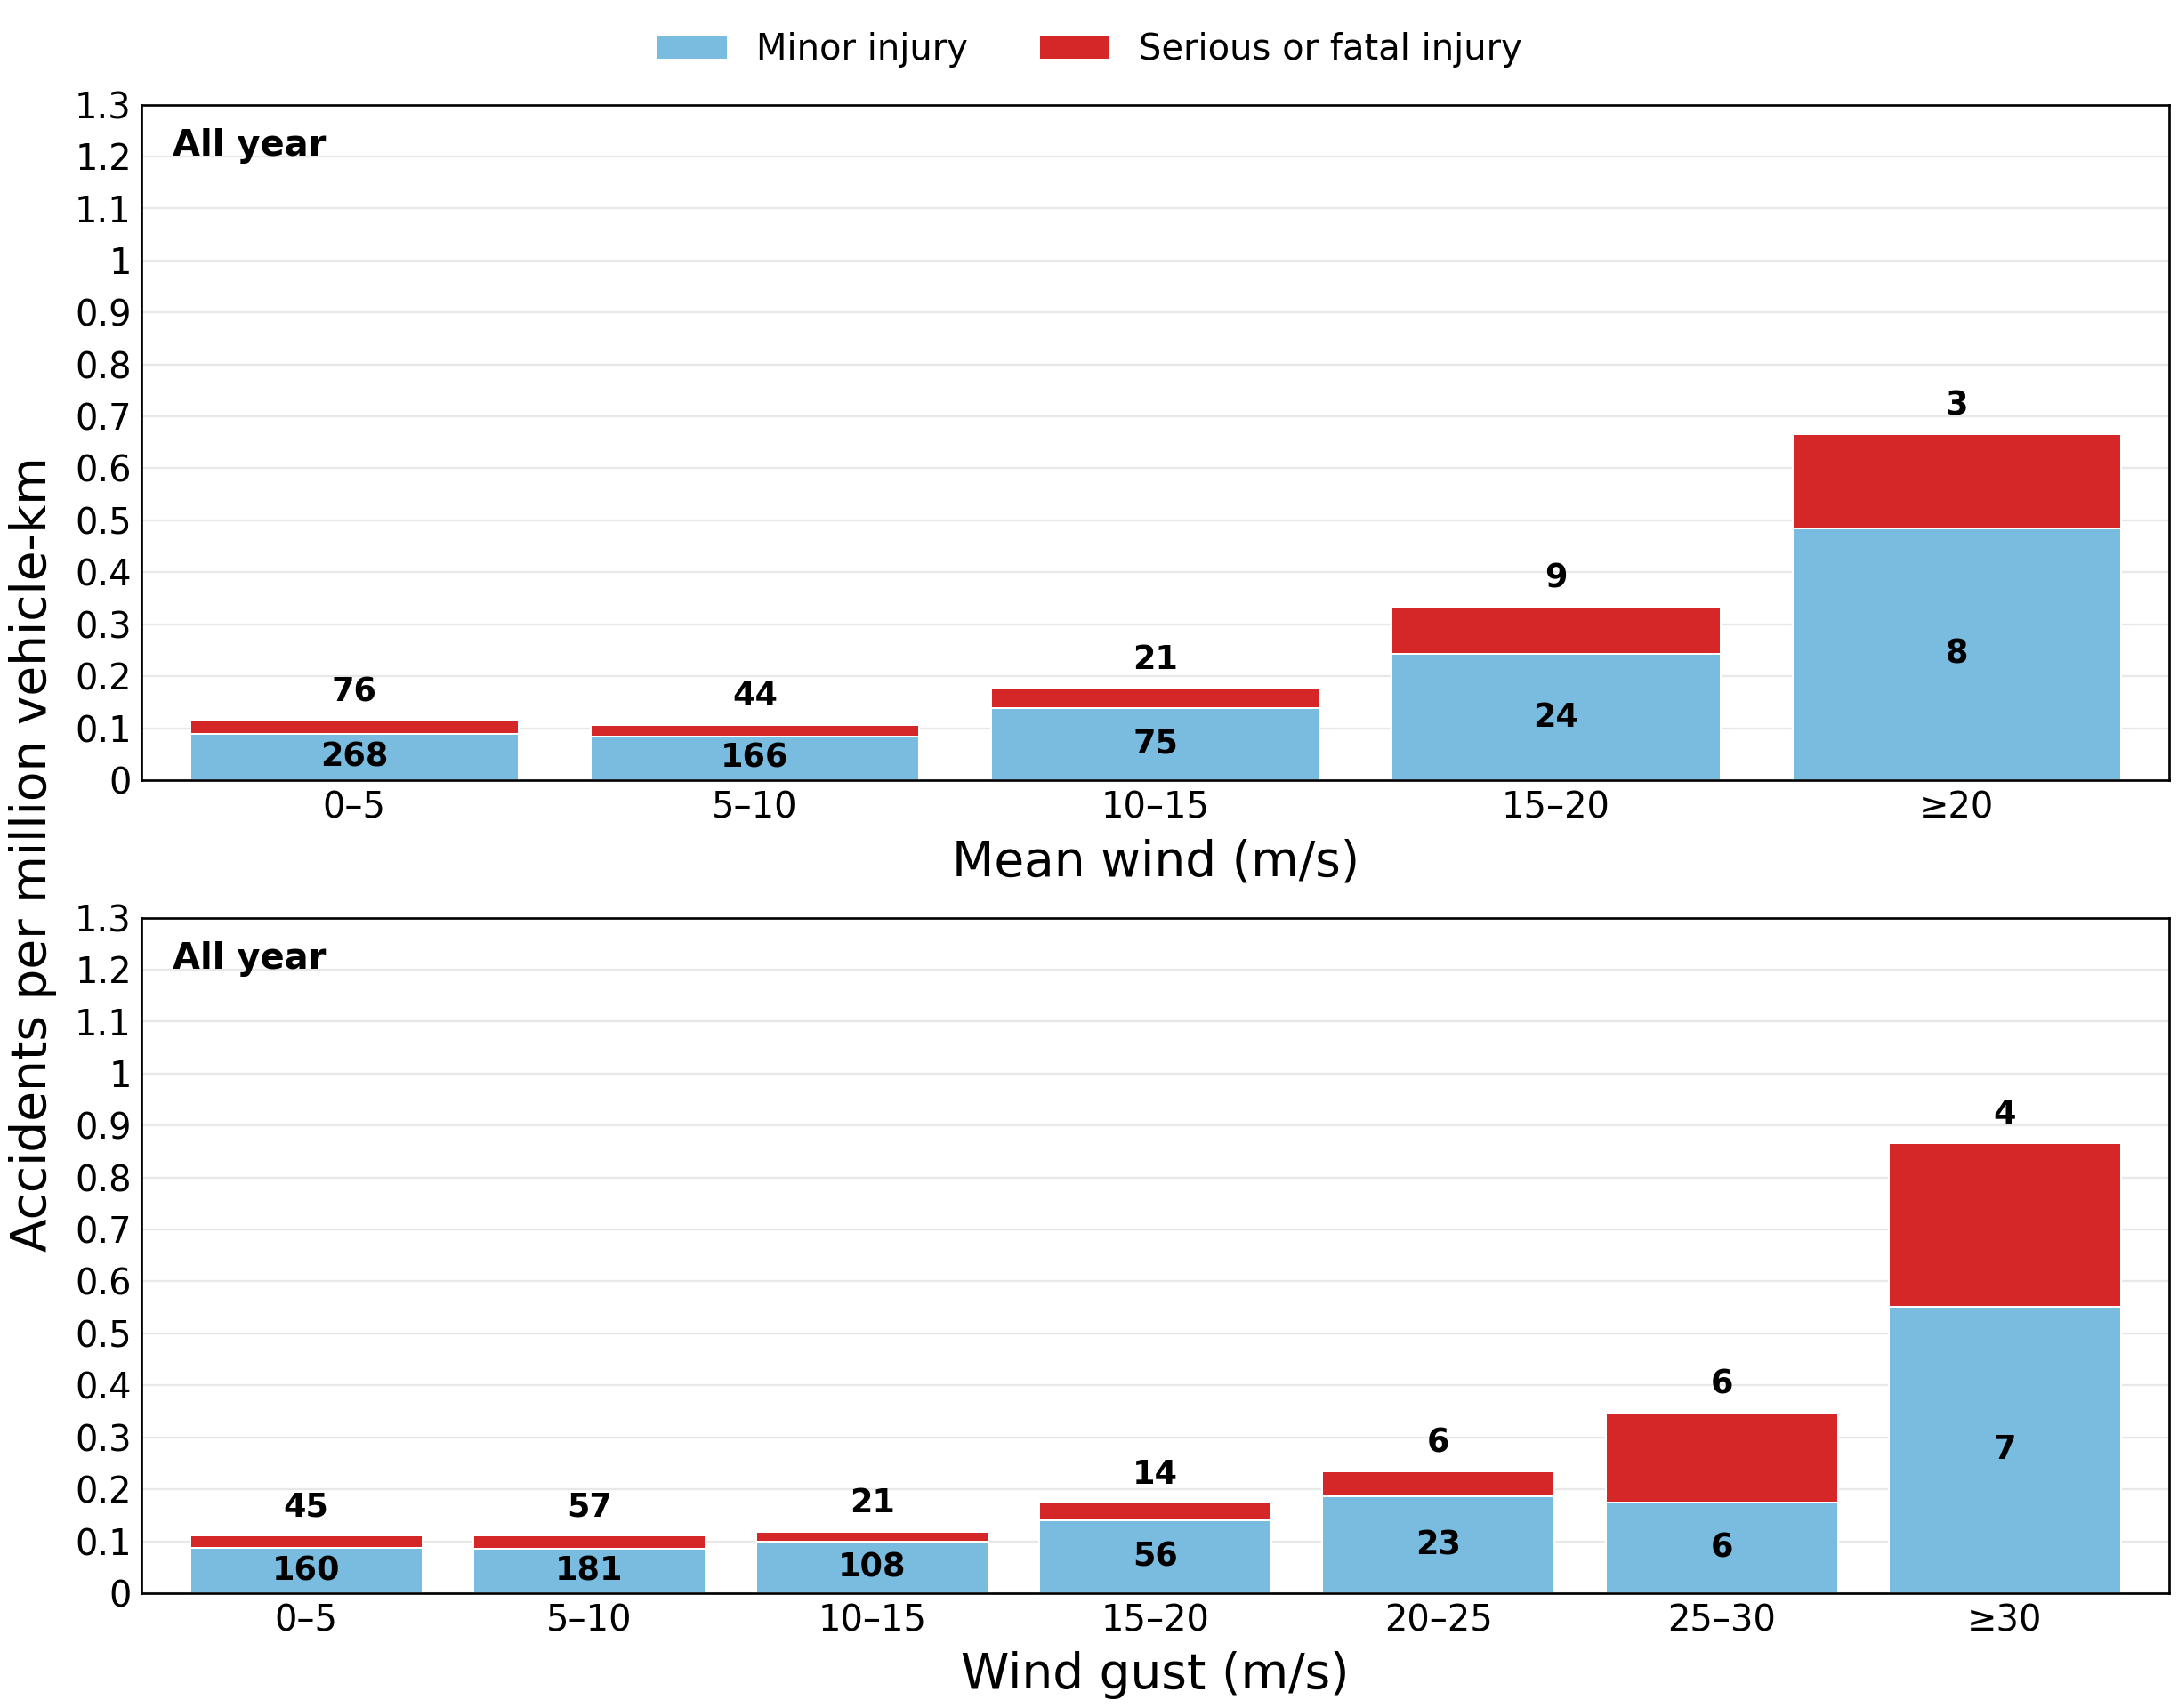
\includegraphics[width=\textwidth,height=0.73\textheight,keepaspectratio]{monthly_weather_rate_annual.png}
\caption[Counter-based wind and gust rates, All year.]{Rural injury-accident
rates per million vehicle-km, 2019--2024, All year. Event-time wind and gust
classify the accidents; daily traffic, rural length and pooled station-month
weather frequencies define estimated exposure. Light blue is minor injury;
red is serious or fatal injury. The stacked components sum to the all-injury
rate; positive labels give counts. Full daily traffic is allocated using
07:00--24:00 weather frequencies; hourly traffic is unobserved.}
\label{fig:monthly-vkt-annual}
\end{figure}
\clearpage

\subsection{Mean Wind by Season}

Figure~\ref{fig:monthly-vkt-wind} shows how the mean-wind pattern varies by
season. Seasonal intervals combine the upper tail at 15 m/s; counts and
exposure are summed before calculating each rate. Blue and red stacks show the minor and serious or fatal components of
each all-injury rate, sharing the same exposure. Positive counts identify
sparse cells; segment sizes are not a formal severity comparison. These panels are descriptive: a season with no observed accident in
an interval is not necessarily free of risk.

\begin{figure}[H]
\centering
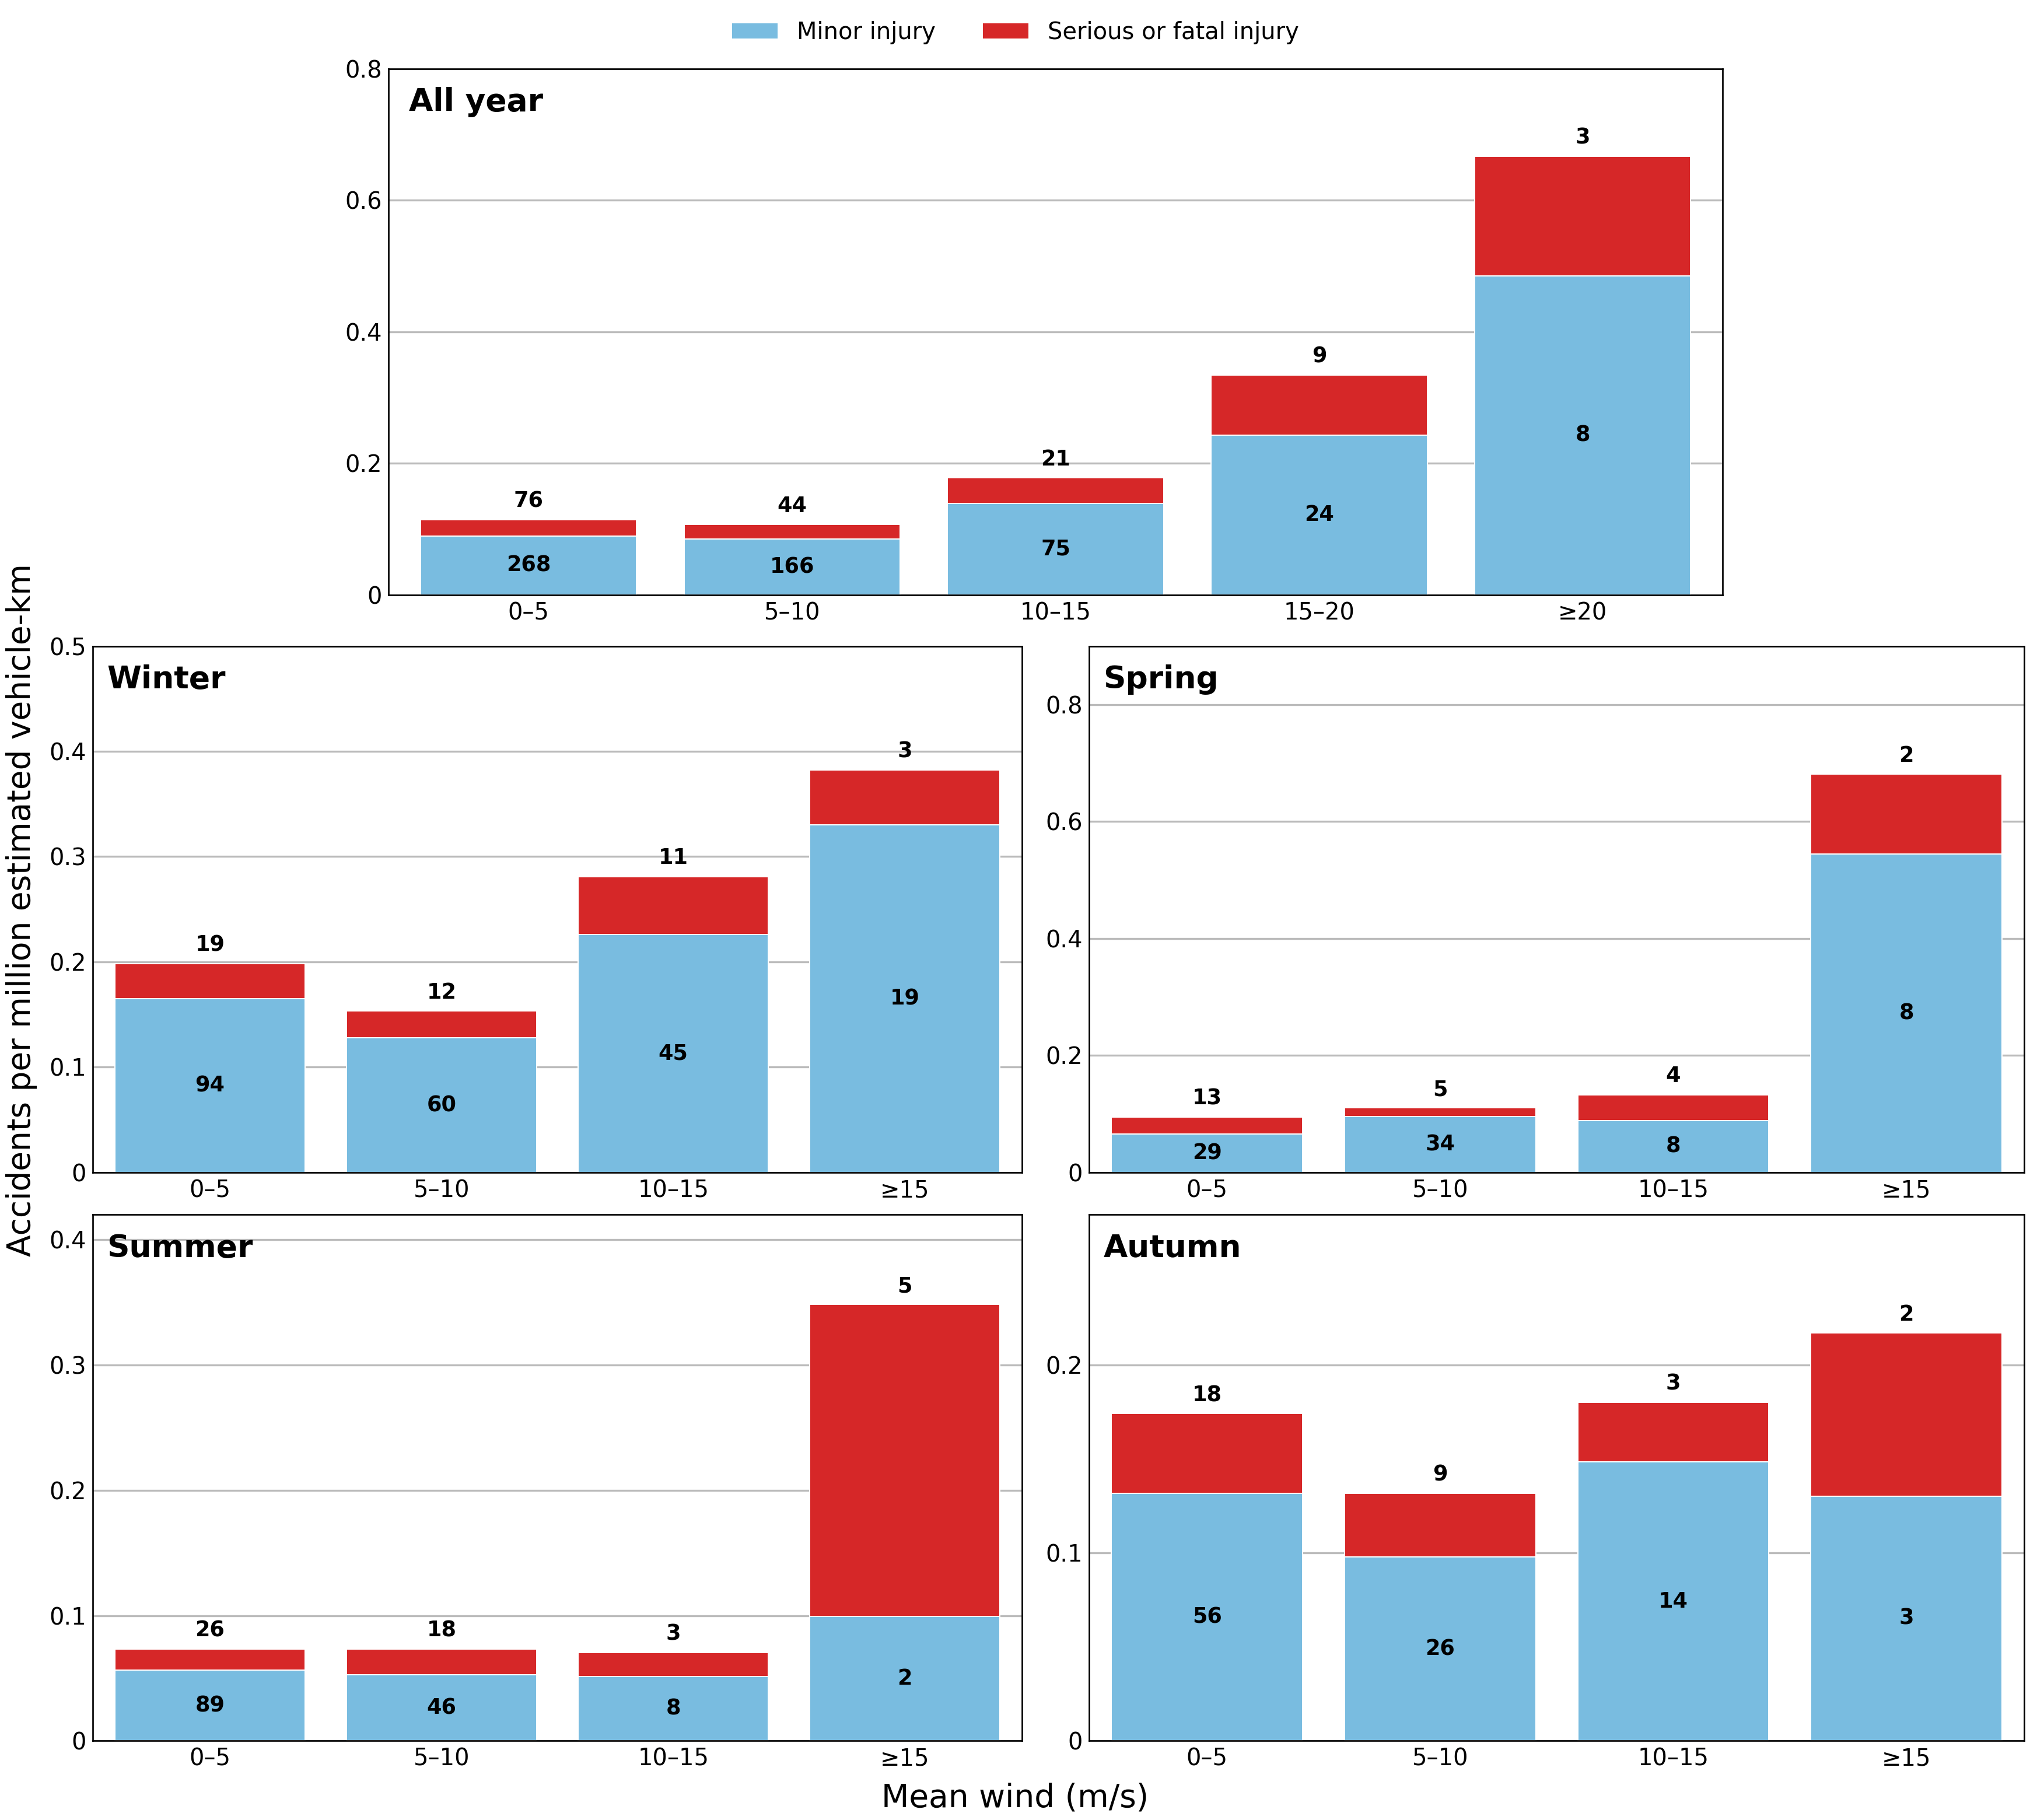
\includegraphics[width=\textwidth,height=0.76\textheight,keepaspectratio]{monthly_f_traffic_rate_panels.png}
\caption[Traffic-based mean wind rates by season.]{Rural injury-accident rates by mean wind, 2019--2024, by season.
Blue is minor injury and red serious or fatal injury; the groups are disjoint.
The stacked components share the same exposure denominator and sum to the
all-injury rate. Estimated vehicle-km use daily traffic, rural length and pooled
monthly weather frequencies. Upper seasonal intervals are combined; labels show positive accident counts;
zero counts are unlabelled. Sparse cells and unobserved hourly traffic limit interpretation.}
\label{fig:monthly-vkt-wind}
\end{figure}

\clearpage
\subsection{Wind Gust by Season}

Figure~\ref{fig:monthly-vkt-gust} shows the corresponding stacked gust pattern,
with seasonal gust intervals combined at 20 m/s.
The upper-bin accidents are spread thinly across seasons, so the panels do
not establish seasonal differences. The main monthly-allocation method supports mean wind and gust only.
Temperature is available in the same-day sensitivity below.

\begin{figure}[H]
\centering
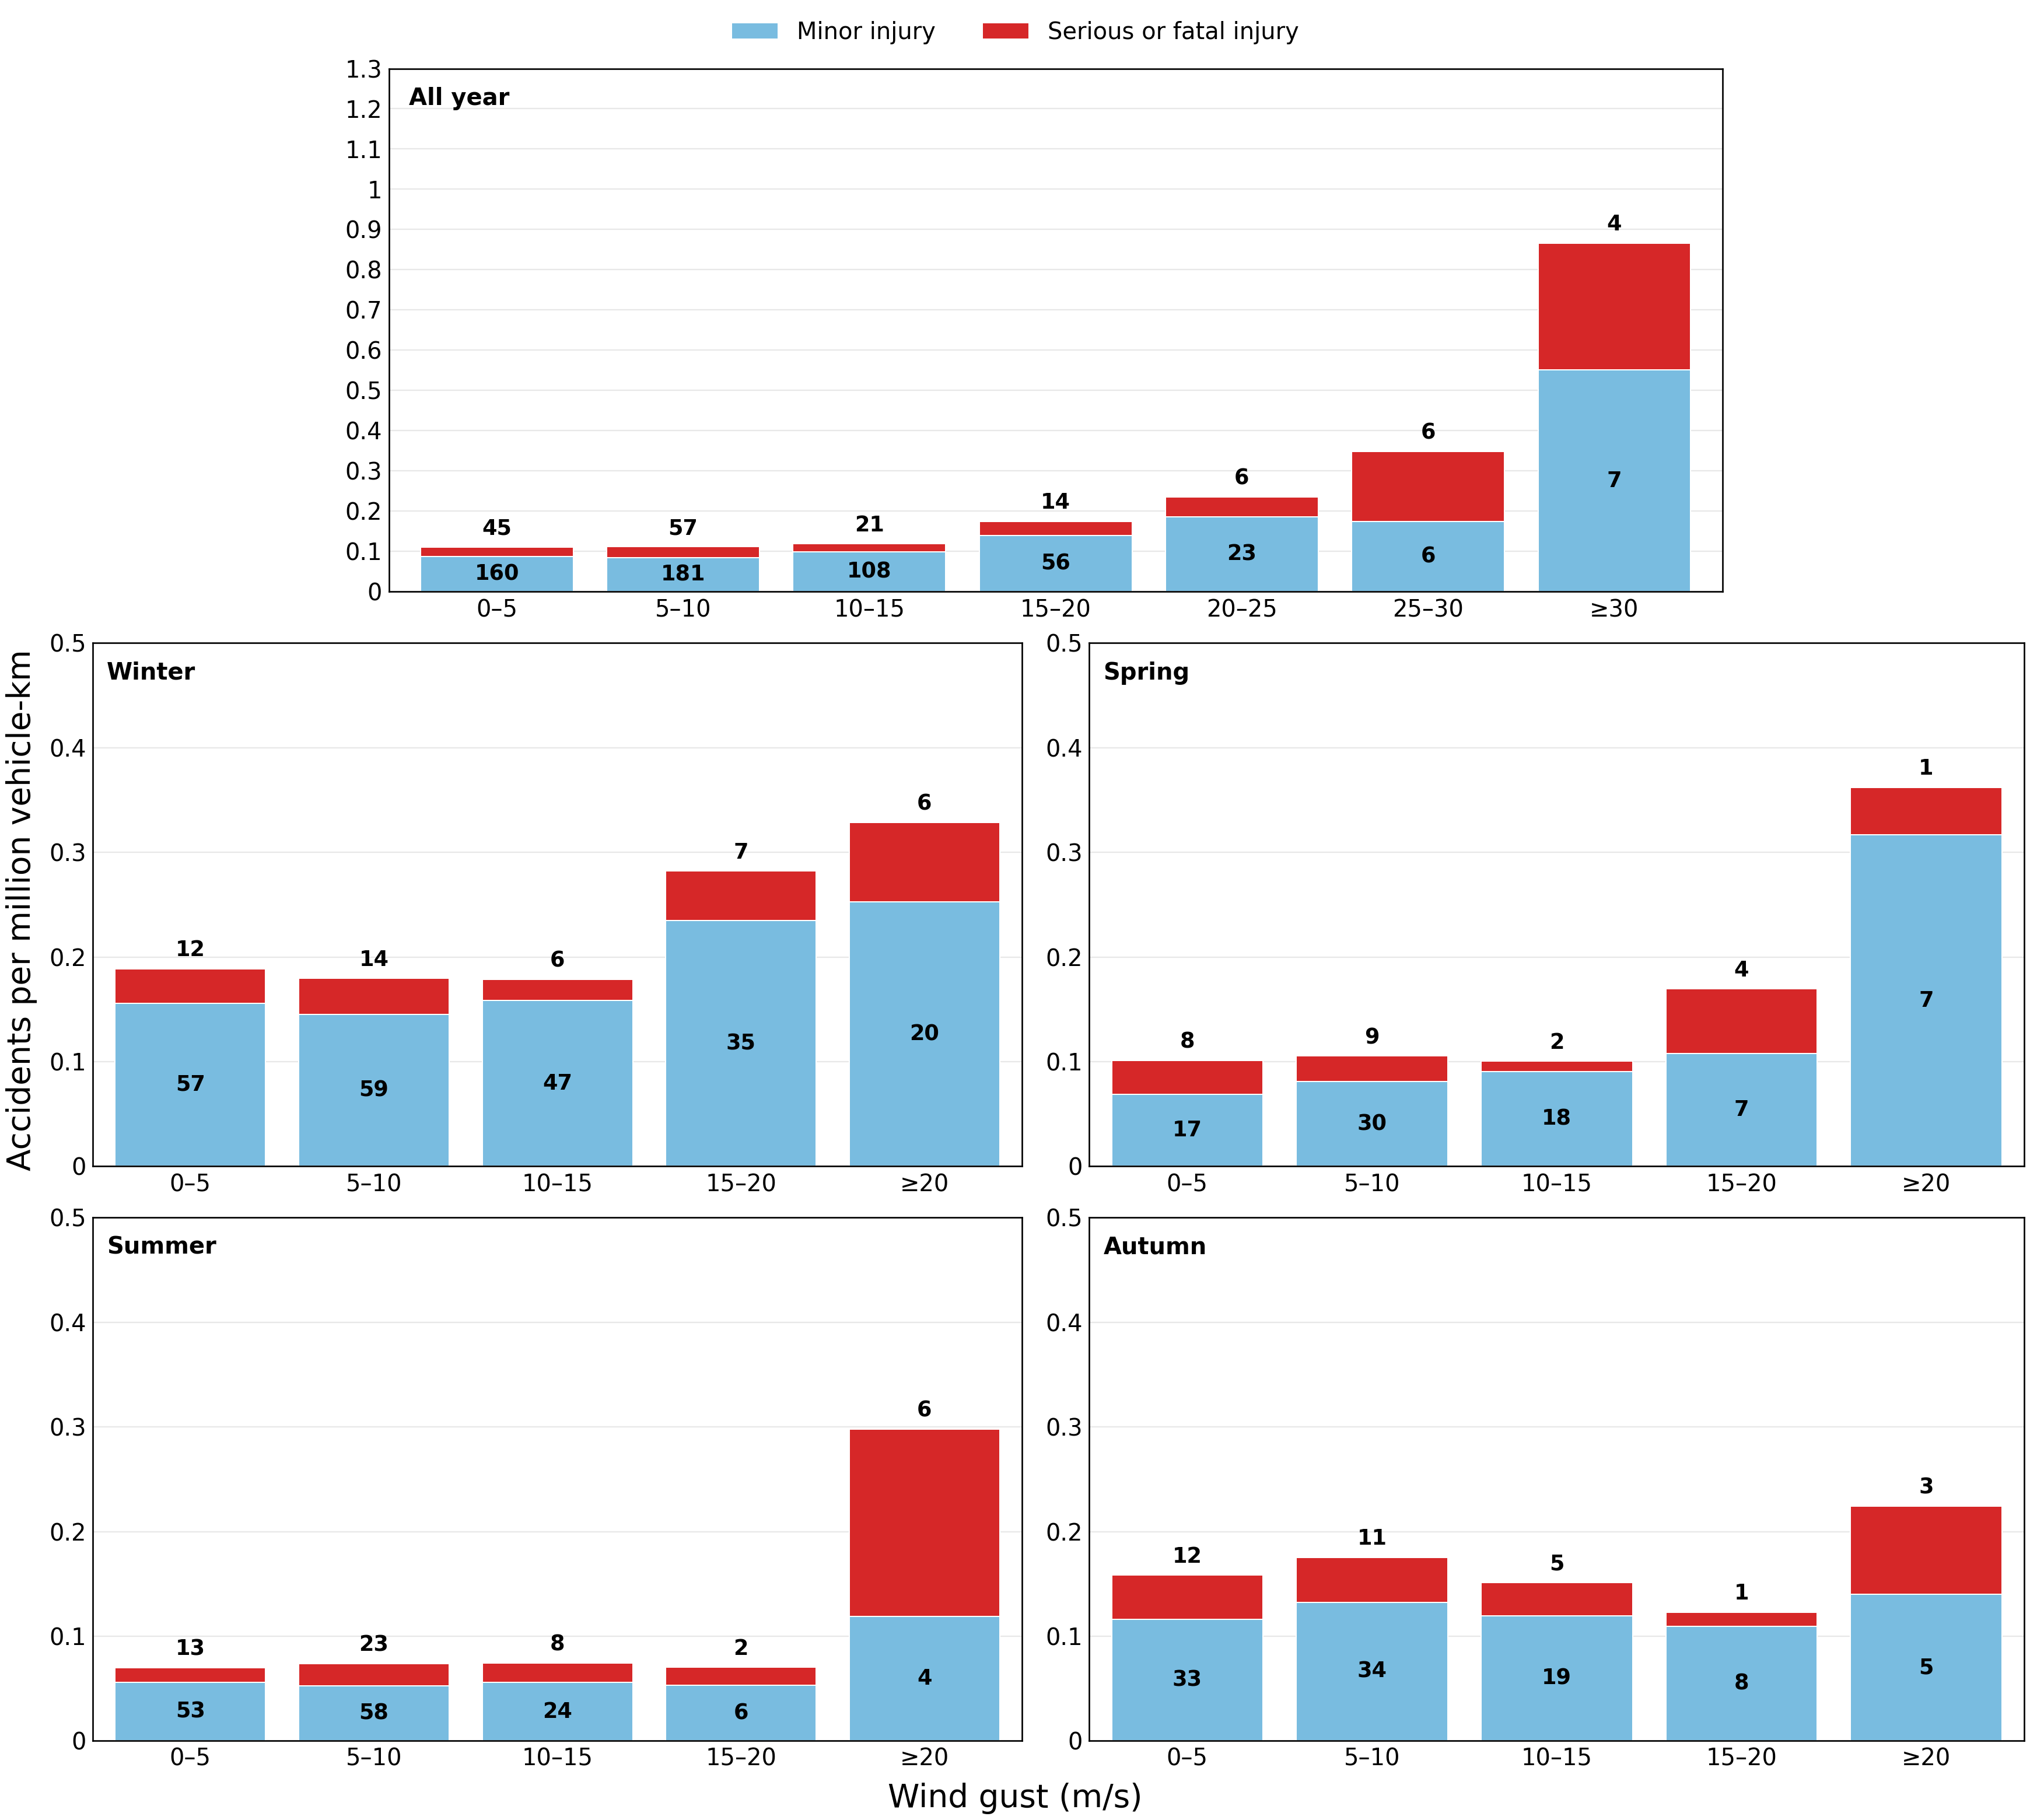
\includegraphics[width=\textwidth,height=0.66\textheight,keepaspectratio]{monthly_fg_traffic_rate_panels.png}
\caption[Traffic-based gust rates by season.]{Rural injury-accident rates by gust, 2019--2024, by season.
Blue is minor injury and red serious or fatal injury; the groups are disjoint.
The stacked components share the same exposure denominator and sum to the
all-injury rate. Estimated vehicle-km use daily traffic, rural length and pooled
monthly weather frequencies. Upper seasonal intervals are combined; labels show positive accident counts;
zero counts are unlabelled. Sparse cells and unobserved hourly traffic limit interpretation.}
\label{fig:monthly-vkt-gust}
\end{figure}
\clearpage

A stratified diagnostic gives smaller upper-bin contrasts when the comparison
is made within counter-section--year--season strata: O/E is 3.39 for mean wind
and 4.84 for gust. This suggests that sample and road-exposure composition
contribute to the larger pooled traffic-based rate ratios. The interpretation of this difference is considered in Chapter~5 rather than treated as a separate
main result here.

Table~\ref{tab:evidence-summary} summarises the headline wind and gust results
for Q1--Q3. Read each estimate against its stated denominator: the table is
an interpretation guide, not a ranking of estimates of one quantity.

\begin{table}[H]
\centering
\small
\caption[Headline wind and gust results.]{Headline mean-wind and gust results. The weather-frequency and approximate traffic-corrected O/E analyses report O/E; the monthly-frequency VKT analysis reports the upper-bin rate divided by the 0--5 m/s rate. The monthly-frequency VKT analysis uses a smaller counter-linked sample, with 11 accidents in each upper interval.}
\label{tab:evidence-summary}
\begin{tabularx}{\textwidth}{L{0.12\textwidth}L{0.17\textwidth}L{0.19\textwidth}L{0.12\textwidth}X}
\toprule
Parameter & Method & Comparison & Estimate & Denominator \\
\midrule
Mean wind & Weather-frequency O/E & $\geq20$ m/s & O/E 2.15 & Local weather frequency \\ \grayhline
Mean wind & Approximate traffic-corrected O/E & $\geq20$ m/s & O/E 2.71 & Traffic-reweighted weather frequency \\ \grayhline
Mean wind & Monthly-frequency VKT & $\geq20$ m/s vs 0--5 & 5.83$\times$ & Estimated VKT (monthly allocation) \\ \grayhline
Wind gust & Weather-frequency O/E & $\geq30$ m/s & O/E 3.34 & Local weather frequency \\ \grayhline
Wind gust & Approximate traffic-corrected O/E & $\geq30$ m/s & O/E 4.20 & Traffic-reweighted weather frequency \\ \grayhline
Wind gust & Monthly-frequency VKT & $\geq30$ m/s vs 0--5 & 7.78$\times$ & Estimated VKT (monthly allocation) \\
\bottomrule
\end{tabularx}
\end{table}


\section{Same-Day Weather Allocation Sensitivity}

Figure~\ref{fig:same-day-annual} and the seasonal Figures~\ref{fig:same-day-wind},
\ref{fig:same-day-gust} and \ref{fig:same-day-temperature} present the same-day
weather allocation sensitivity. These figures test sensitivity to the allocation assumption; the monthly-frequency
method remains the main traffic-rate analysis. The same 694 linked accidents are classified by
accident-time weather, but exposure follows the weather observed on each
counter-day and excludes unobserved weather time. The resulting rates therefore
have a different denominator from the monthly method. Their agreement in the
broad wind pattern is more informative than a direct comparison of magnitudes.

\begin{figure}[p]
\centering
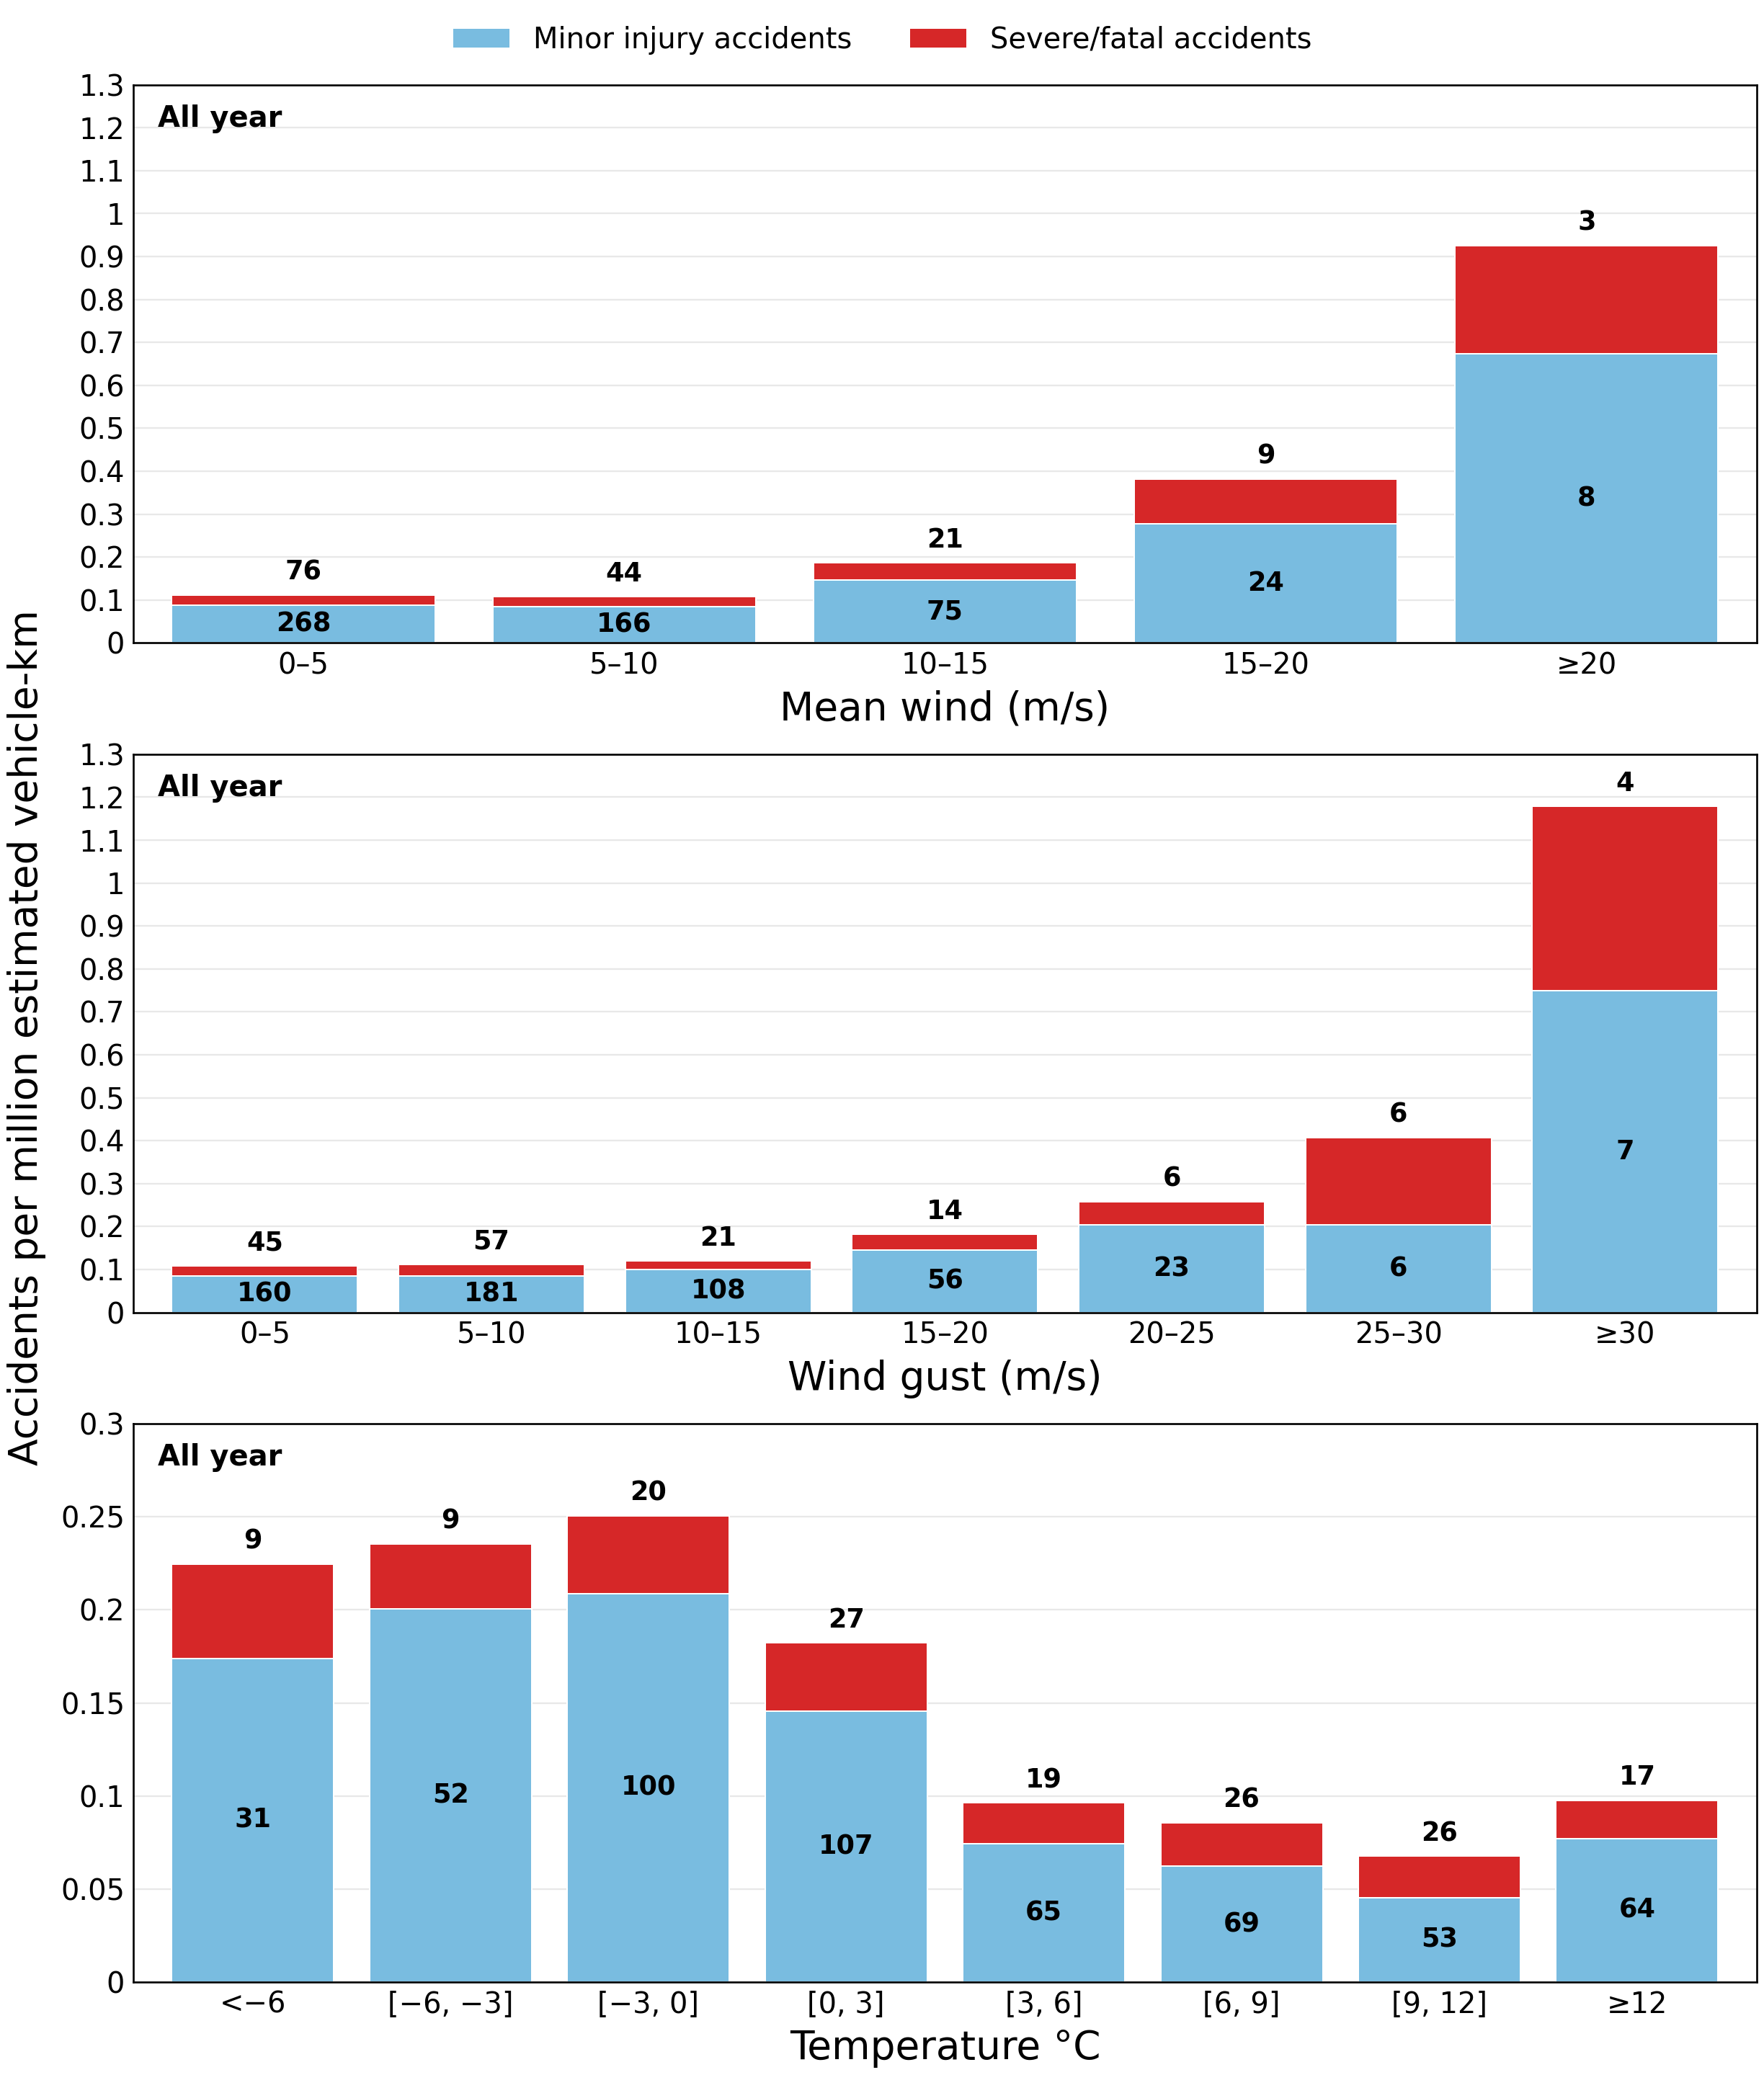
\includegraphics[width=\textwidth,height=0.76\textheight,keepaspectratio]{weather_rate_annual.png}
\caption[Same-day weather allocation sensitivity, All year.]{Same-day weather allocation sensitivity
for rural injury accidents, 2019--2024, All year. The numerator uses event-time
weather; exposure is daily traffic times rural length times observed bin minutes
within 07:00--24:00 divided by 1,020. Unobserved weather minutes contribute no
exposure. Light-blue minor and red serious or fatal rates share this denominator;
positive labels give counts. Parameter-specific scales follow the original
presentation. Daily counts do not measure hourly traffic.}
\label{fig:same-day-annual}
\end{figure}

The wind and gust seasonal plots combine upper intervals to reduce sparse cells:
mean wind ends at 15 m/s or above and gust at 20 m/s or above. All year retains
the finer intervals. Temperature retains its existing intervals throughout.
This difference in binning must be considered before comparing panel heights;
no seasonal rank or causal effect follows from the largest bar.

\begin{figure}[p]
\centering
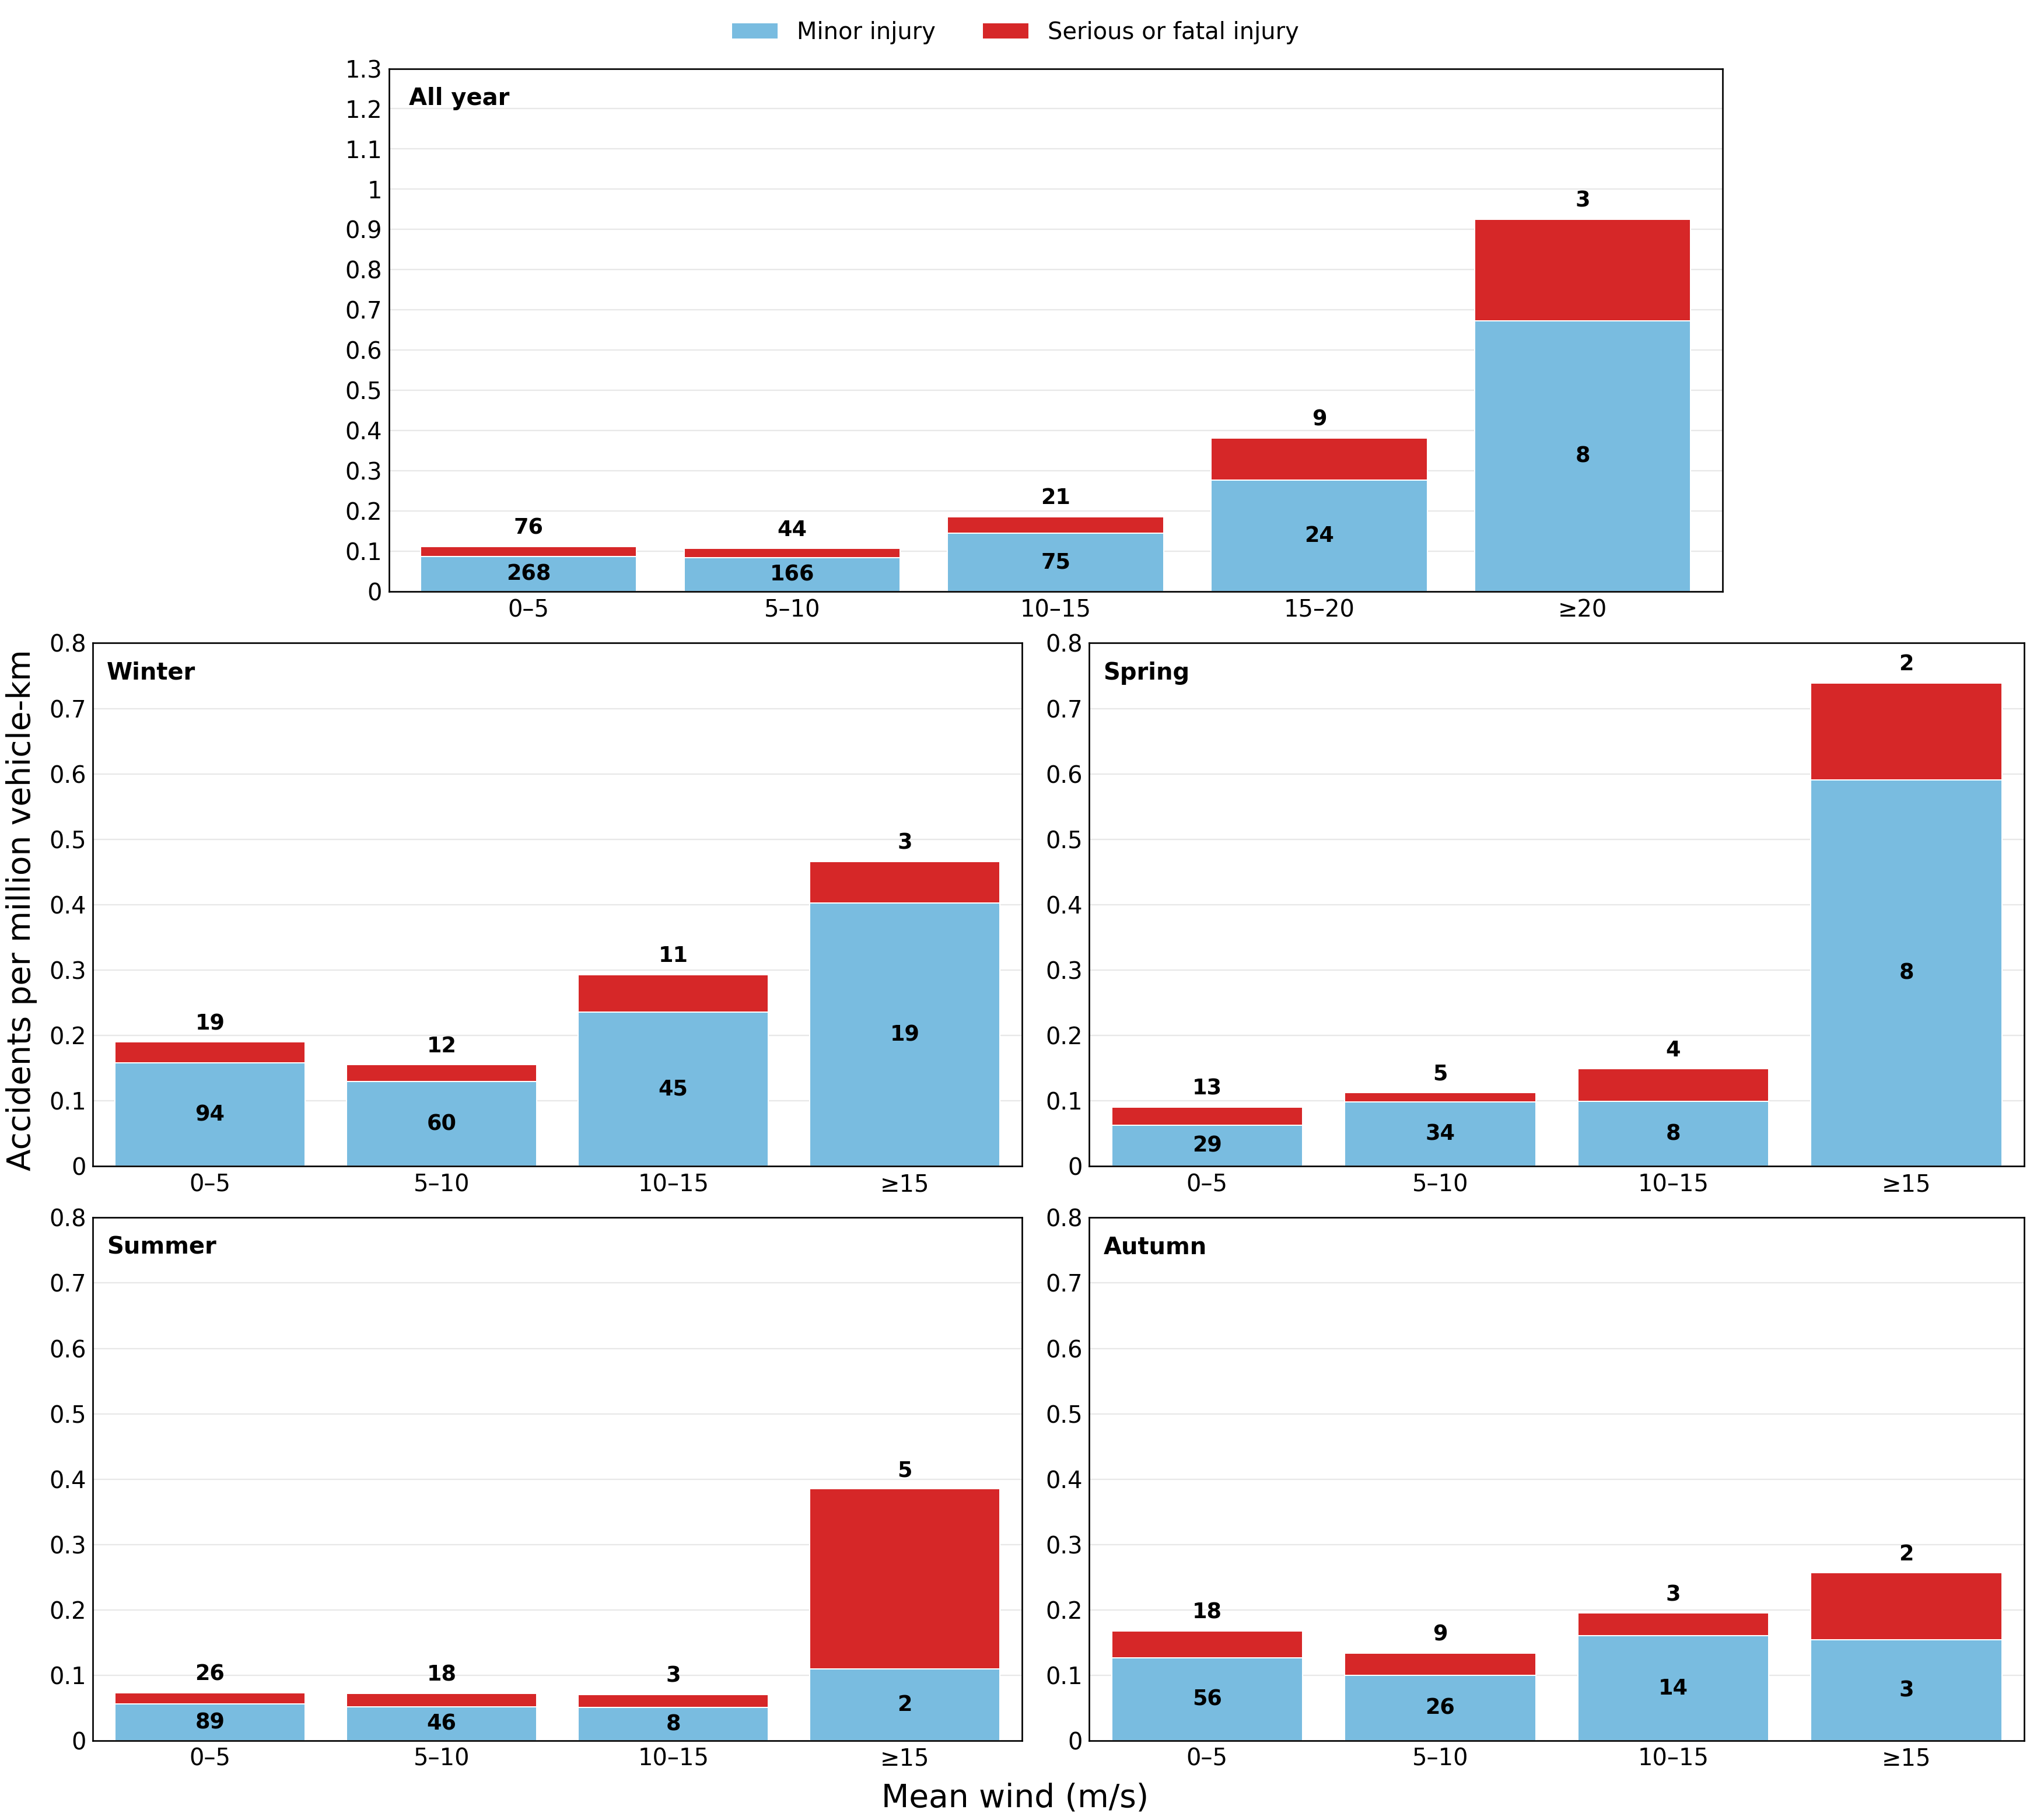
\includegraphics[width=\textwidth,height=0.76\textheight,keepaspectratio]{f_traffic_rate_panels.png}
\caption[Same-day mean-wind allocation sensitivity by season.]{Same-day mean-wind accident rates per million vehicle-km,
2019--2024. Estimated exposure allocates daily traffic using that day's
07:00--24:00 weather, excluding unobserved weather time. Blue and red stacks
show minor injury and serious or fatal injury; readable positive counts are
labelled. Seasonal upper bins are combined as described in the text. This is a sensitivity to same-day rather than monthly exposure allocation.}
\label{fig:same-day-wind}
\end{figure}

\begin{figure}[p]
\centering
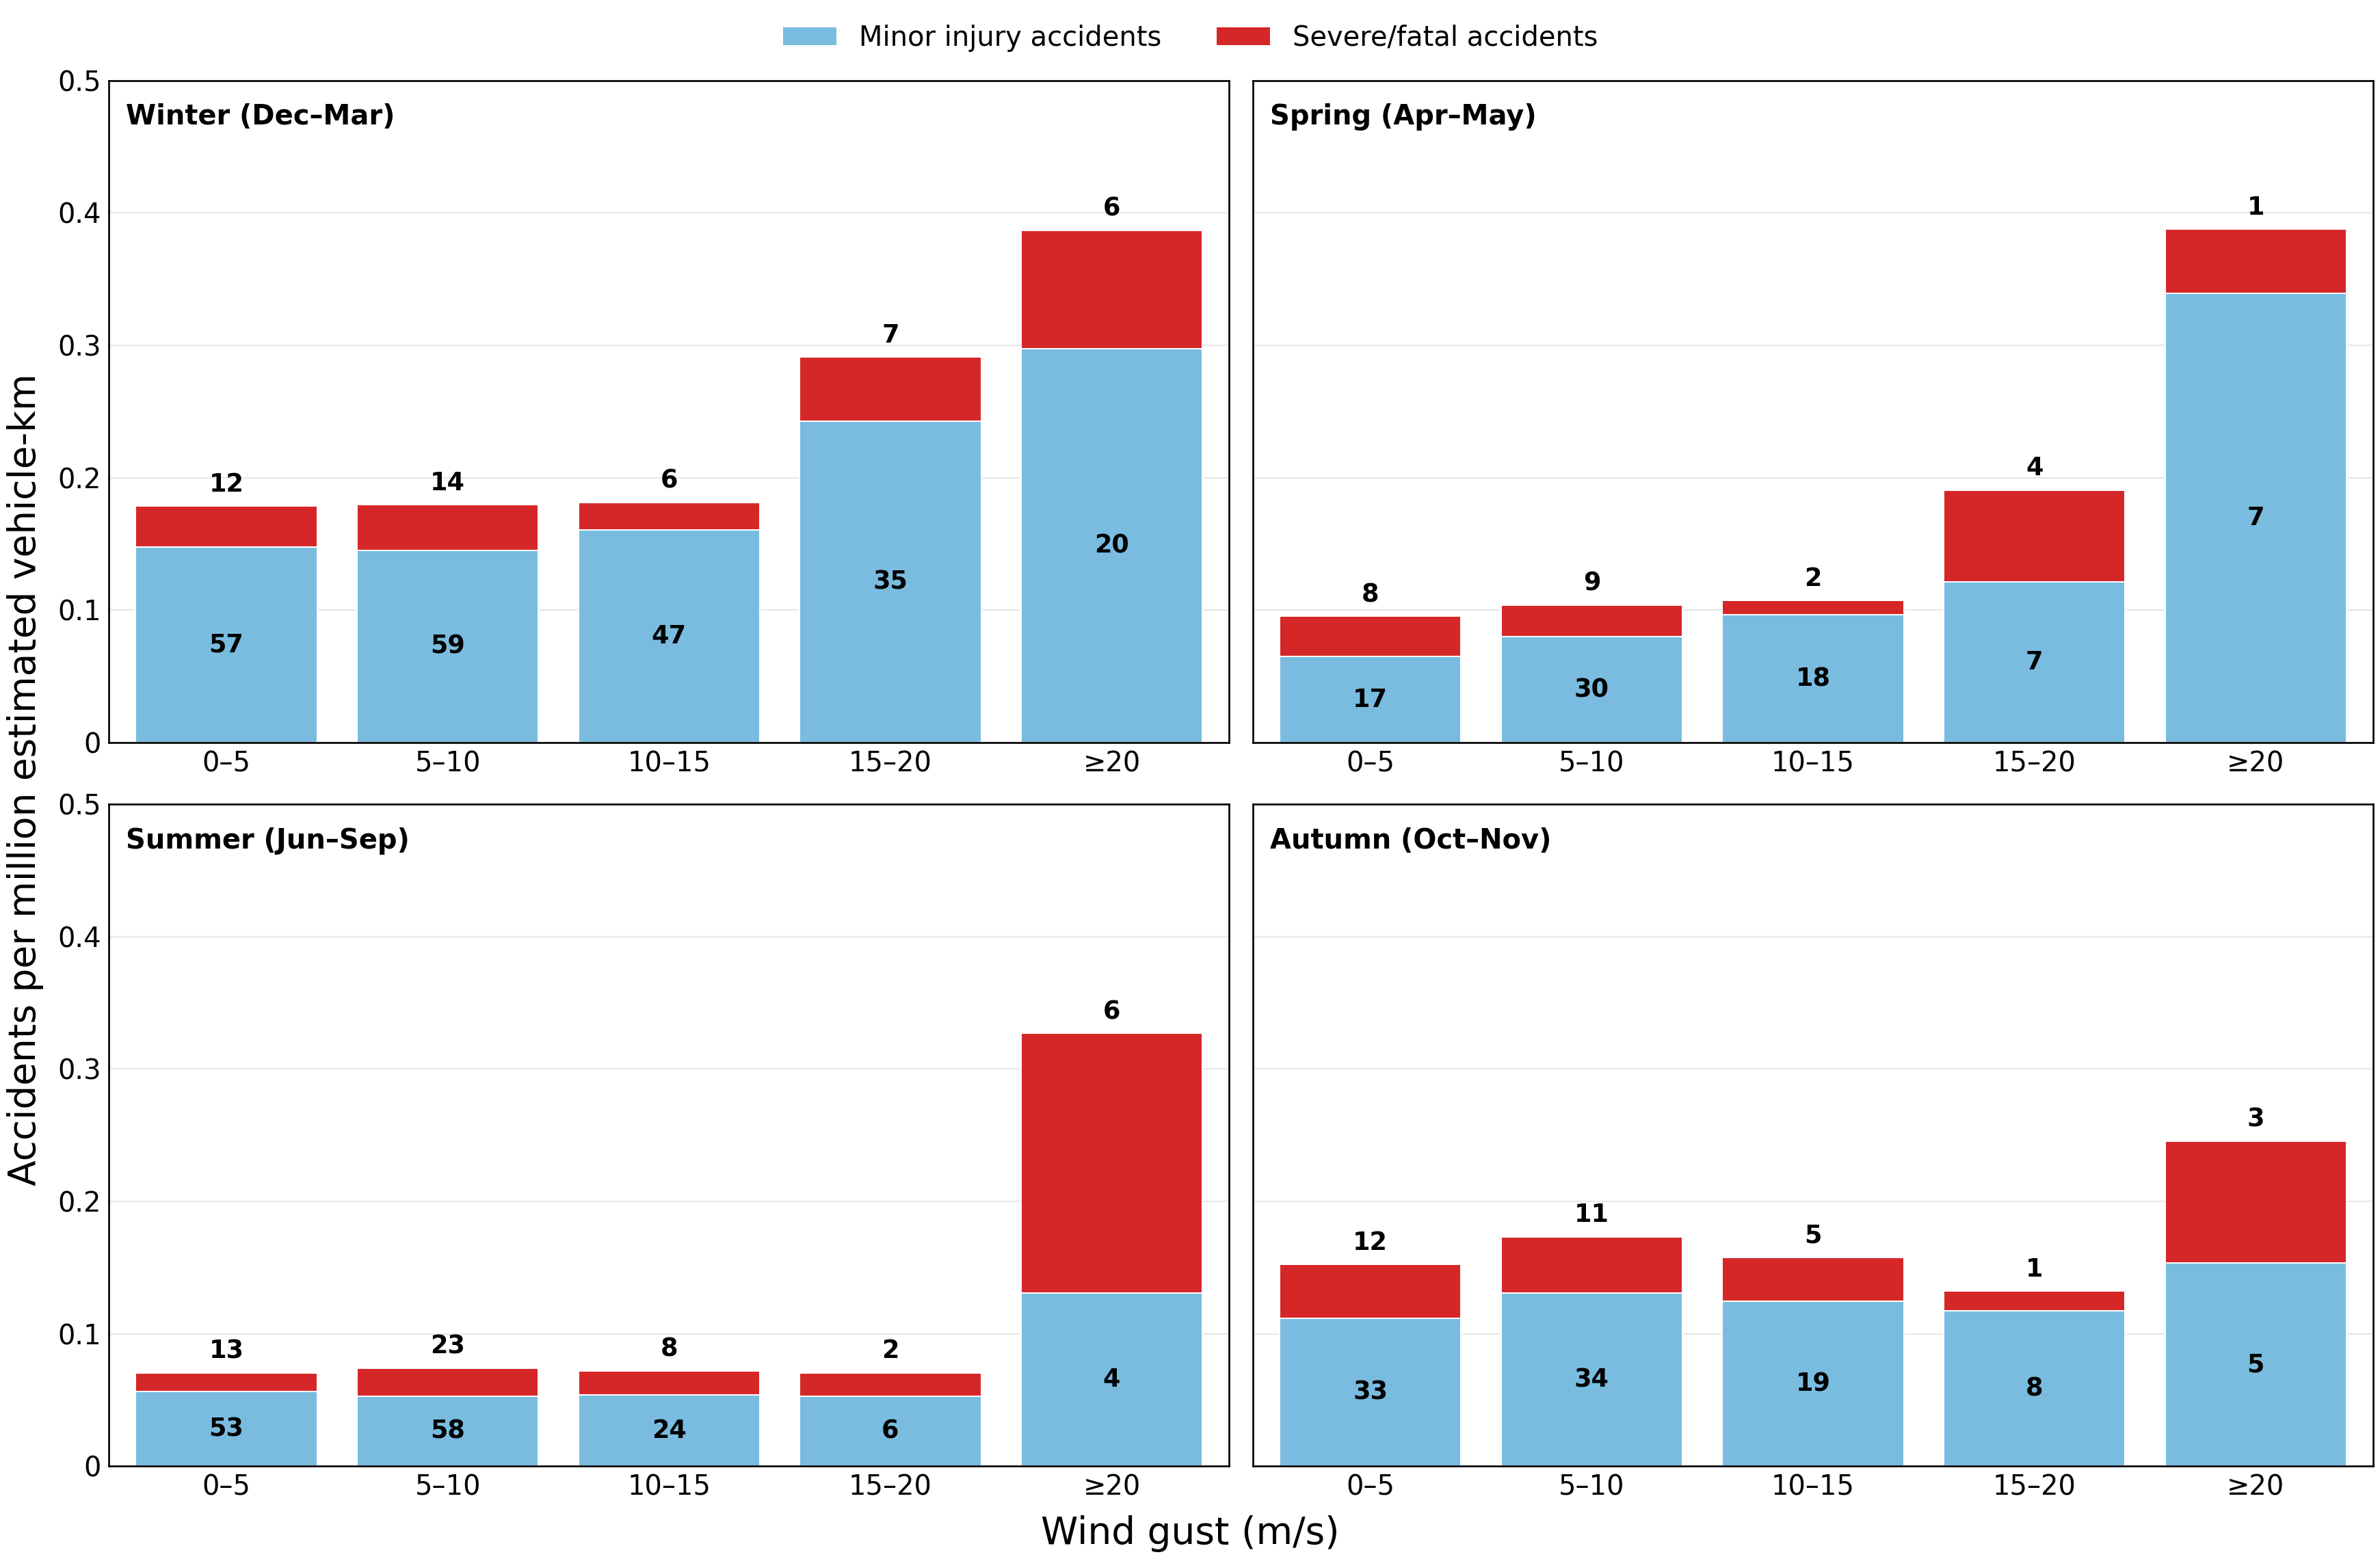
\includegraphics[width=\textwidth,height=0.76\textheight,keepaspectratio]{fg_traffic_rate_panels.png}
\caption[Same-day gust allocation sensitivity by season.]{Same-day wind-gust accident rates per million vehicle-km,
2019--2024. Estimated exposure allocates daily traffic using that day's
07:00--24:00 weather, excluding unobserved weather time. Blue and red stacks
show minor injury and serious or fatal injury; readable positive counts are
labelled. Seasonal upper bins are combined as described in the text. This is a sensitivity to same-day rather than monthly exposure allocation.}
\label{fig:same-day-gust}
\end{figure}

\begin{figure}[p]
\centering
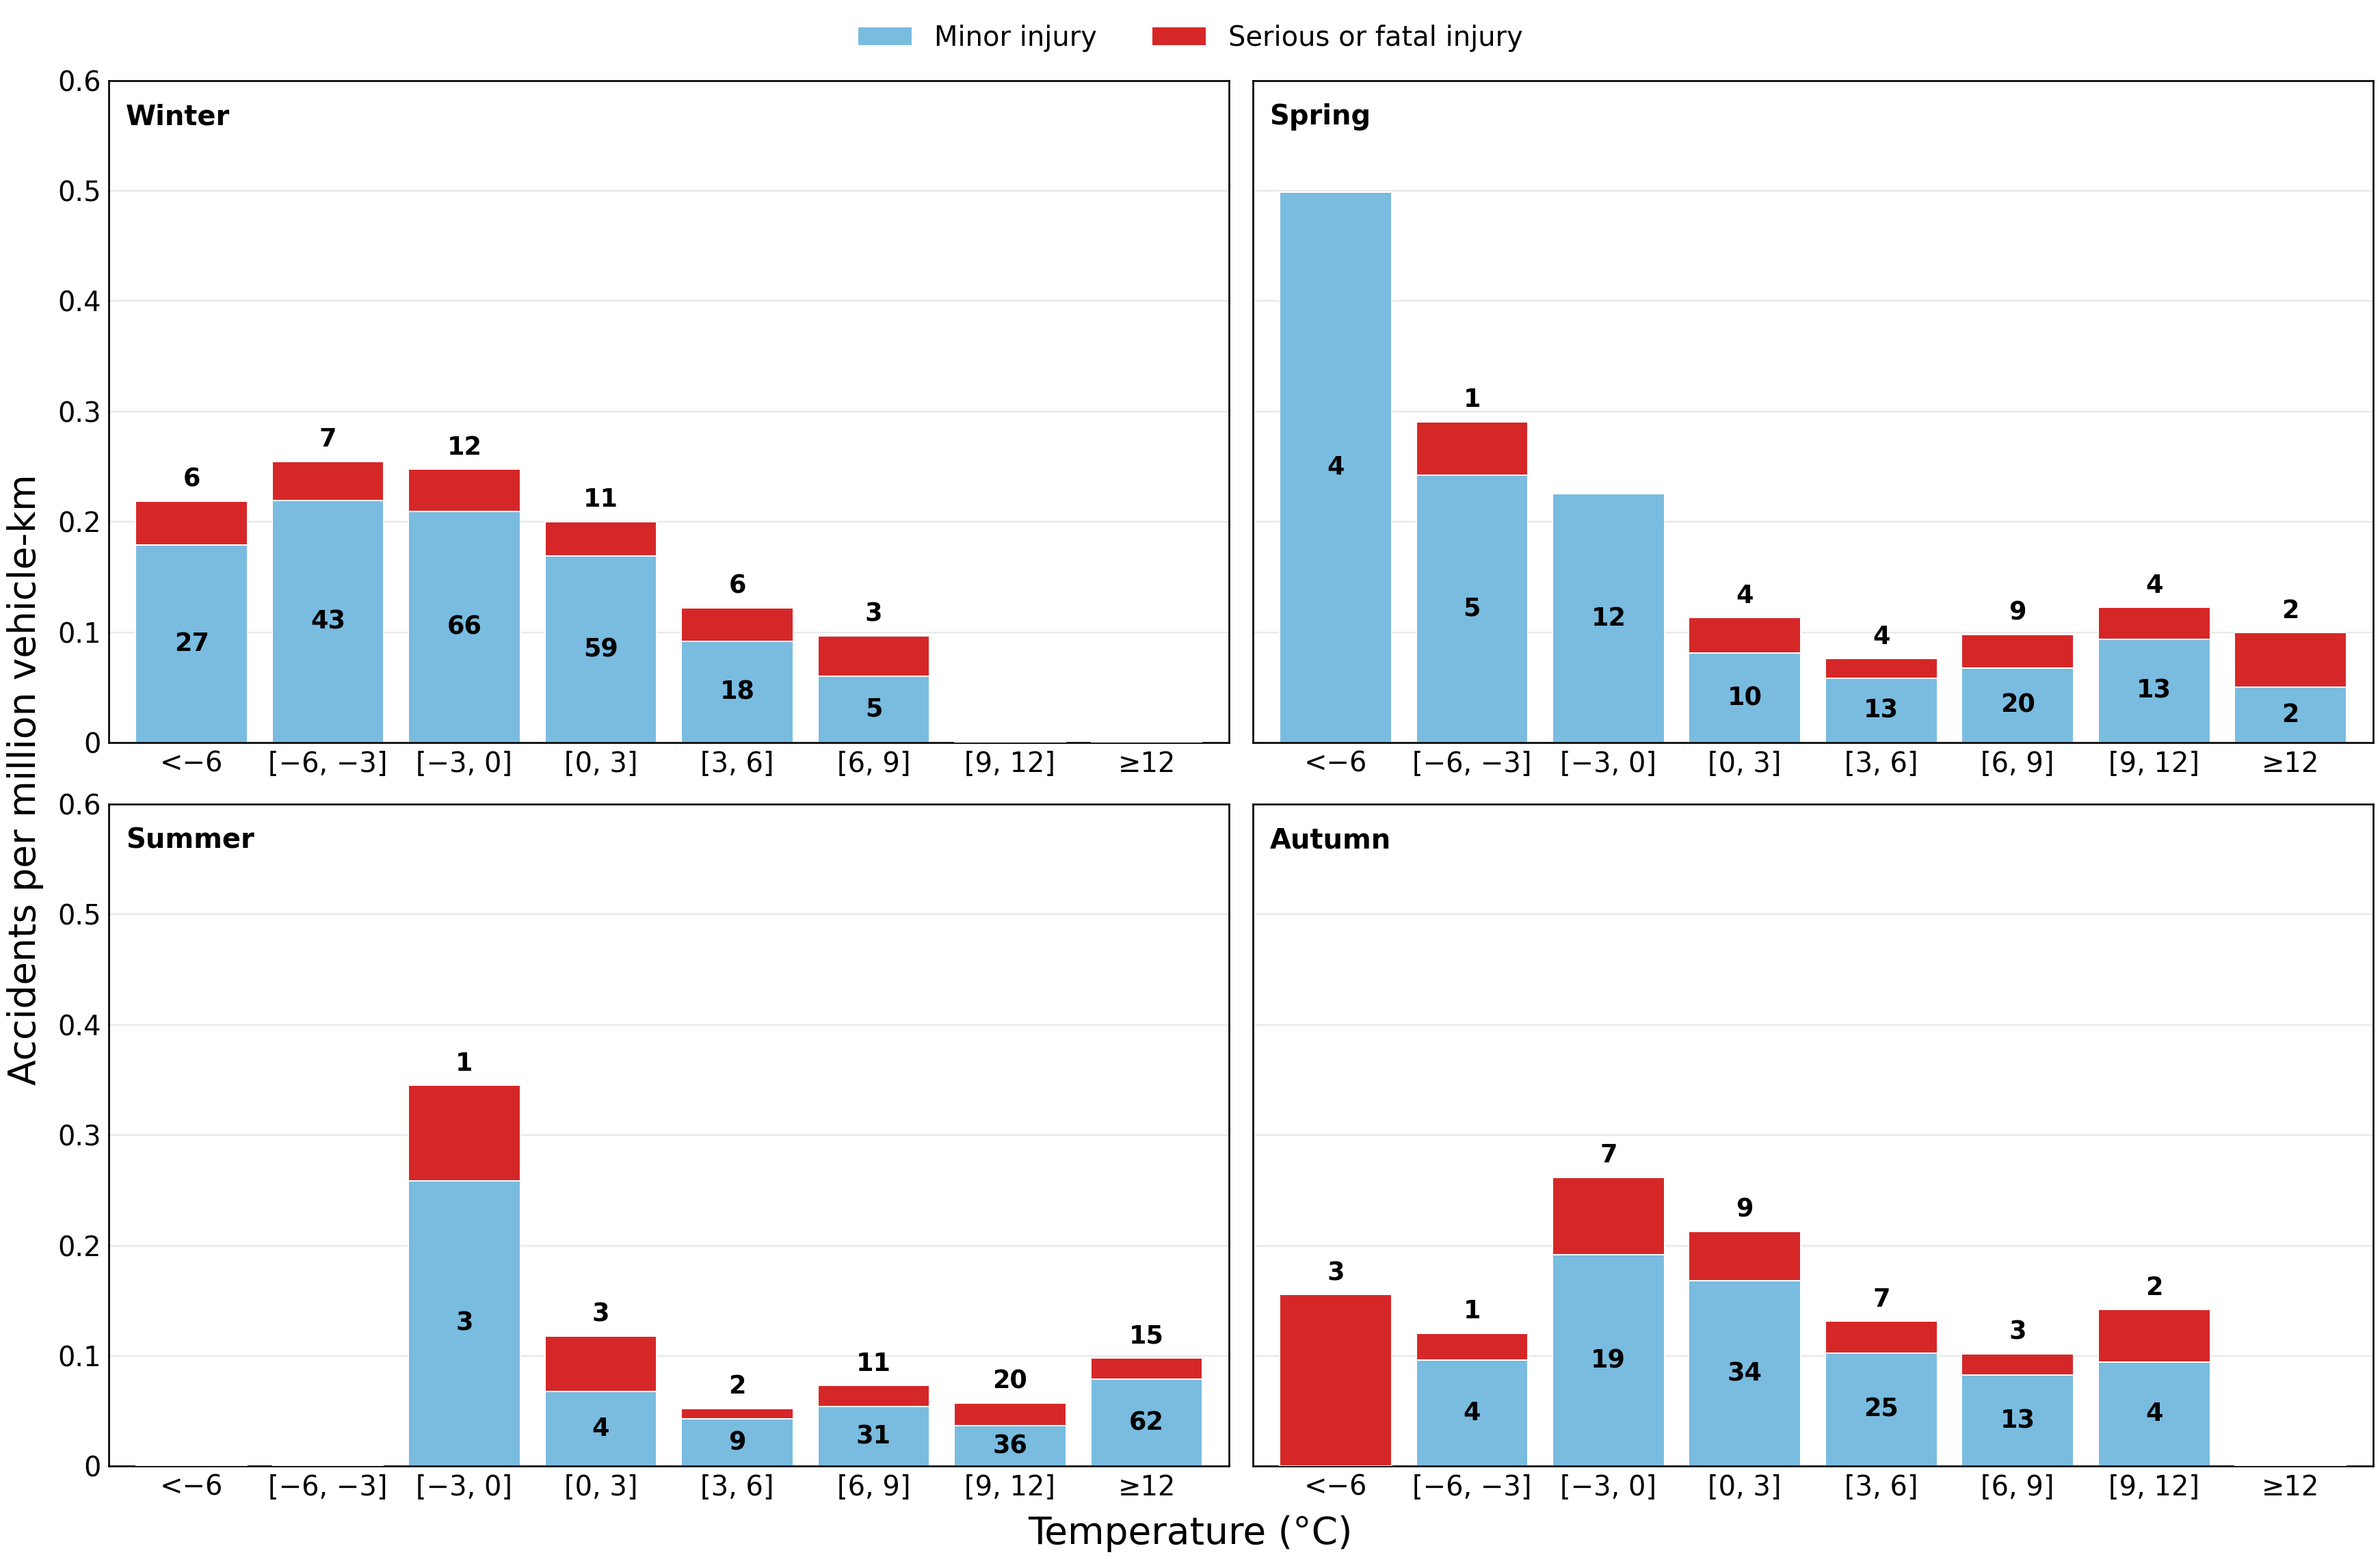
\includegraphics[width=\textwidth,height=0.76\textheight,keepaspectratio]{temperature_traffic_rate_panels.png}
\caption[Same-day temperature allocation sensitivity by season.]{Same-day temperature accident rates per million vehicle-km,
2019--2024. Estimated exposure allocates daily traffic using that day's
07:00--24:00 weather, excluding unobserved weather time. Blue and red stacks
show minor injury and serious or fatal injury; readable positive counts are
labelled. This is a sensitivity to same-day rather than monthly exposure allocation.}
\label{fig:same-day-temperature}
\end{figure}

\clearpage

\section{Secondary Robustness Checks}

These checks use different statistical conditioning or distinct traffic
models. The period and allocation sensitivities above directly address Q2
and Q3; the following checks test other aspects of the wind association.

\subsection{Matched-Time and Secondary Weather Checks}

The matched-time comparison tests whether the wind pattern persists after
controlling for station and recurring calendar time.
Table~\ref{tab:matched-time-summary} shows an upper-wind association, with
lower and moderate contrasts near one. This check does not control unusual
traffic or road conditions on a particular day.

\begin{table}[H]
\centering
\small
\caption[Selected matched-time contrasts.]{Selected matched-time contrasts. Each model uses 6,257 accident strata; the joint wind contrast includes temperature. Intervals are 95\% confidence intervals.}
\label{tab:matched-time-summary}
\begin{tabularx}{\textwidth}{Xrr}
\toprule
Comparison & OR & 95\% CI \\
\midrule
Mean wind: $\geq$15 vs 0--5 m/s & 1.61 & 1.38--1.87 \\ \grayhline
Mean wind, with temperature: $\geq$15 vs 0--5 m/s & 1.68 & 1.44--1.96 \\ \grayhline
Gust: $\geq$30 vs 0--10 m/s & 2.74 & 1.96--3.85 \\ \grayhline
Temperature: $-3$--0 vs 0--3 $^{\circ}$C & 1.13 & 1.02--1.25 \\ \grayhline
Temperature: 3--6 vs 0--3 $^{\circ}$C & 0.59 & 0.53--0.65 \\ \grayhline
Temperature: $\geq$15 vs 0--3 $^{\circ}$C & 0.99 & 0.80--1.23 \\
\bottomrule
\end{tabularx}
\end{table}


The gust model also rises in the upper intervals, whereas the temperature
results remain non-monotonic. Including temperature in the mean-wind model
changes the upper-wind estimate only slightly. The
matched-time temperature result reproduces the dip at moderate temperatures but
not the warm-end increase seen in Q1, reinforcing the cautious interpretation
of temperature.

Daylight and severity provide additional context. Few matched sets change
daylight class, making those estimates imprecise. The adjusted severity model
provides no clear evidence of greater severity during strong wind once an
injury accident has occurred (Appendix Table~\ref{tab:severity-conditions}).
A matched-time wind-by-season interaction is detectable, but sparse upper-wind
cells do not support ranking individual seasons.

\subsection{Supporting Traffic Models}

The annual road-section model and the allocated daily-counter model also
show higher rates in strong wind. Their samples and exposure constructions
differ from Q1--Q3, so agreement in direction is more informative than their
relative magnitudes. Appendix Table~\ref{tab:traffic-sensitivity} reports the
numerical sensitivity checks, including restrictions to official traffic
periods and exclusion of recorded zero counter-days.

\chapter{Discussion}

\section{Interpretation}

The analyses consistently place the strongest contrasts in the upper wind
intervals. Q1 establishes over-representation relative to local weather
frequency; Q2 asks whether reduced traffic explains it; Q3 relates accidents
to estimated distance travelled on counter-linked roads. Their agreement in
direction matters more than agreement in magnitude because they measure
different quantities.

Q2 addresses an important limitation of weather-frequency O/E: traffic volume
is not constant across weather conditions. At the selected counters, daily
traffic is lower during stronger wind. If that response also applies to the
broader rural road network, weighting expected accidents by the observed
traffic response makes the upper-wind contrast larger rather than explaining it
away. The correction remains approximate, however. It extrapolates a
2019--2024 counter relationship to the 2007--2025 primary population, and it
uses daily traffic totals rather than traffic observed in the same 10-minute
intervals used to classify accidents. Q2 is therefore best interpreted as a
sensitivity analysis of the primary O/E rather than as a measured
traffic-adjusted accident rate.

Q3 incorporates day-to-day traffic variation directly in the denominator, but
its larger rate ratio requires separate interpretation. The sample covers
only roads and years with usable counter information, and the upper wind
intervals contain few accidents. In addition, pooled
vehicle-kilometre rates can be influenced by which road sections contribute
exposure to each wind interval. A diagnostic comparison within
counter-section--year--season strata gives smaller contrasts than the pooled
Q3 rate ratios. This suggests that differences in road and exposure composition
account for part of the larger pooled contrasts. It does not establish that
particular roads are intrinsically more dangerous, and the sparse upper bins
leave substantial uncertainty about the exact magnitude of the contrast.

Monthly-frequency allocation is the preferred main denominator for the available
daily traffic totals. Same-day allocation is shown as a sensitivity because it
uses realised daily weather. Agreement in the high-wind pattern supports the
direction of the association, while differences in magnitude are expected from
the different allocations. Neither method observes hourly traffic.

The supporting analyses are consistent with this interpretation but answer
different questions. The matched-time comparison retains an upper-wind
association after controlling for station and recurring calendar time. This
makes an explanation based solely on regular differences between months,
weekdays or times of day less plausible. Gust shows a similar upper-tail
pattern, although mean wind and gust are related measurements from the same
weather observations. Temperature is less consistent: its O/E pattern is
non-monotonic and the matched-time analysis does not reproduce the warm-end
increase. The severity model likewise gives no clear evidence that strong wind
is associated with a greater probability of serious or fatal injury once an
injury accident has occurred. These results support a distinction between the
occurrence of accidents and their severity.

The main wind result is consistent with earlier work comparing accident shares
with the time spent in adverse weather \citep{edwards1994} and with engineering
research showing mechanisms by which crosswind can impair vehicle stability
\citep{baker1986,baker1994risk}. The contribution here is not a new physical
wind threshold, but a long Icelandic accident series linked to local weather
frequency and then examined under several complementary exposure
constructions. The non-monotonic temperature findings are also consistent with
previous evidence that temperature associations can vary by range and season
\citep{lee2014,zhan2020}, while the observed reduction in traffic during strong
wind agrees with recorder-based evidence that adverse weather changes travel
demand \citep{sathiaraj2018}.

\section{Strengths}

A principal strength is the broad primary sample: rural injury accidents
are linked to quality-controlled 10-minute weather observations, and expected
counts are standardised within weather station and study season rather than
against a single national weather distribution. Match coverage, observed
counts and weather-quality exclusions are reported explicitly, which makes the
primary O/E calculation transparent and auditable.

The exposure analyses complement rather than replace this broad comparison.
Q2 tests how the primary result changes under an empirically estimated traffic
response, while Q3 uses observed daily traffic, road length and all eligible
counter-days, including days without an accident. The matched-time and additional traffic models provide supporting checks under
different conditioning and exposure assumptions. Keeping these analyses separate makes their assumptions
visible instead of combining incompatible data sources into one apparently
precise measure. Documented transformations, automated tests and stage-specific
audits further support reproducibility.

\section{Limitations}

The main limitation is incomplete traffic exposure. Q1 uses weather time rather
than vehicle-kilometres. Q2 introduces traffic only through an approximate
response estimated from selected counters in 2019--2024 and extrapolated to the
broader 2007--2025 population. The counter data are daily totals, so neither Q2
nor Q3 observes how many vehicles were travelling during the specific
10-minute weather interval in which an accident occurred.

Q3 is more exposure-based but also more selective. It is limited to rural
counter sections with usable traffic, road geometry and weather in 2019--2024.
The full observed daily count is allocated to 07:00--24:00 using pooled
station-month weather frequencies, an assumption that preserves daily exposure
but does not reconstruct hourly traffic. The monthly weather frequencies use
the longer 2007--2025 weather record for stability, while the traffic and
accidents themselves are restricted to 2019--2024. Few Q3 accidents occur
in the highest mean-wind and gust intervals, so the corresponding large
rate ratios should be interpreted as directional evidence rather than precise
estimates. An assigned counter also represents exposure on a road section; it
does not establish that the vehicle involved in an accident passed that
counter.

Weather measurement introduces a separate source of uncertainty. A station up
to 20 km from an accident or counter location is a proxy for conditions on the
road, and Icelandic terrain can produce substantial variation over shorter
distances. The five-minute matching rule can also select an observation on the
adjacent calendar day for accidents close to midnight; this preserves the time
tolerance but should be understood as part of the matching definition. The
fixed 2020--2024 urban-boundary dataset is applied to the full 2007--2025
accident period, so historical changes in settlement boundaries are not
represented.

The supporting models have their own restrictions. The case-crossover design
controls recurring calendar time but not unusual traffic, road-surface
conditions, visibility or closures on a particular day. The annual traffic
model distributes seasonal traffic across wind intervals using weather
frequency rather than observed wind-specific traffic. More generally, all
analyses are observational. Unmeasured road characteristics, vehicle type,
speed, visibility, driver behaviour and weather-related road management may
contribute to the observed patterns. The study therefore supports associations
and exposure contrasts, not causal effects of wind.

\section{Future Work}

The most valuable extension would be verified hourly traffic linked to stable
counter coordinates, road-section identifiers, direction information and
counter downtime. Hourly exposure would remove the need to distribute daily
traffic totals across weather intervals and would allow accident-time weather
to be paired with traffic measured at a compatible temporal resolution. A
second useful extension would examine baseline accident rates and exposure
composition across road sections to determine how much of the difference
between pooled traffic-based rates and locally standardised O/E is attributable to road
mix. With sufficiently detailed data, vehicle class, road geometry and wind
direction relative to the road could also be incorporated.

\chapter{Conclusion}

Strong wind is over-represented at rural injury-accident times in Iceland
relative to how often it occurs locally. At mean wind speeds of at least
20 m/s, the primary observed-to-expected ratio is 2.15. Gust shows a similar
pattern, while temperature associations are less consistent.

Accounting approximately for reduced traffic strengthens the wind contrast.
The separate traffic-based rate analysis points in the same direction, but
covers a smaller, more selective road sample and has few accidents in the
highest wind intervals. Road and exposure composition appear to explain part of its
larger contrast.

These findings support an association, not a causal effect of wind or a direct
national estimate of accident risk per distance travelled. Broader counter
coverage and hourly traffic measurements are needed to estimate that risk
without relying on within-day exposure assumptions.

\begin{thebibliography}{23}

\bibitem[Ahmed et al.(2012)]{ahmed2012}
Ahmed, M. M., Abdel-Aty, M., and Yu, R. (2012).
\newblock Assessment of interaction of crash occurrence, mountainous freeway
geometry, real-time weather, and traffic data.
\newblock \emph{Transportation Research Record}, 2280(1), 51--59.
\newblock \url{https://doi.org/10.3141/2280-06}.

\bibitem[Andrey et al.(2003)]{andrey2003}
Andrey, J., Mills, B., Leahy, M., and Suggett, J. (2003).
\newblock Weather as a chronic hazard for road transportation in Canadian cities.
\newblock \emph{Natural Hazards}, 28, 319--343.

\bibitem[Baker(1986)]{baker1986}
Baker, C. J. (1986).
\newblock A simplified analysis of various types of wind-induced road vehicle
accidents.
\newblock \emph{Journal of Wind Engineering and Industrial Aerodynamics}, 22(1), 69--85.
\newblock \url{https://doi.org/10.1016/0167-6105(86)90012-7}.

\bibitem[Baker(1994)]{baker1994risk}
Baker, C. J. (1994).
\newblock The quantification of accident risk for road vehicles in cross winds.
\newblock \emph{Journal of Wind Engineering and Industrial Aerodynamics}, 52, 93--107.
\newblock \url{https://doi.org/10.1016/0167-6105(94)90041-8}.

\bibitem[Edwards(1994)]{edwards1994}
Edwards, J. B. (1994).
\newblock Wind-related road accidents in England and Wales 1980--1990.
\newblock \emph{Journal of Wind Engineering and Industrial Aerodynamics}, 52, 293--303.
\newblock \url{https://doi.org/10.1016/0167-6105(94)90055-8}.

\bibitem[Hagstofa Íslands(2026)]{hagstofaThettbyli}
Hagstofa Íslands. (2026).
\newblock Urban-locality geographic data, 2020--2024.
\newblock \url{https://gis.is/geoserver/Hagstofan/ows}.

\bibitem[Hrafnkelsdóttir(2020)]{hrafnkelsdottir2020}
Hrafnkelsdóttir, E. (2020).
\newblock \emph{Effects of wind on vehicles: Development of a calculation model}
(in Icelandic).
\newblock Vegagerðin research report 1800-707-2.
\newblock \url{https://www.vegagerdin.is/vegagerdin/gagnasafn/skyrslur/utgefnar-rannsoknaskyrslur/umferd/2020-umferd/ahrif-vinds-a-farartaeki-throun-reiknilikans/}.

\bibitem[Janes et al.(2005)]{janes2005}
Janes, H., Sheppard, L., and Lumley, T. (2005).
\newblock Case-crossover analyses of air pollution exposure data: Referent
selection strategies and their implications for bias.
\newblock \emph{Epidemiology}, 16(6), 717--726.
\newblock \url{https://doi.org/10.1097/01.ede.0000181315.18836.9d}.

\bibitem[Johansson et al.(2009)]{johansson2009}
Johansson, \"O., Wanvik, P. O., and Elvik, R. (2009).
\newblock A new method for assessing the risk of accident associated with darkness.
\newblock \emph{Accident Analysis \& Prevention}, 41(4), 809--815.
\newblock \url{https://doi.org/10.1016/j.aap.2009.04.003}.

\bibitem[Lee et al.(2014)]{lee2014}
Lee, W.-K., Lee, H. A., Hwang, S.-S., Kim, H., Lim, Y.-H., Hong, Y.-C.,
Ha, E.-H., and Park, H. (2014).
\newblock A time series study on the effects of cold temperature on road
traffic injuries in Seoul, Korea.
\newblock \emph{Environmental Research}, 132, 290--296.
\newblock \url{https://doi.org/10.1016/j.envres.2014.04.019}.

\bibitem[Lord and Mannering(2010)]{lord2010}
Lord, D. and Mannering, F. (2010).
\newblock The statistical analysis of crash-frequency data: a review and
assessment of methodological alternatives.
\newblock \emph{Transportation Research Part A: Policy and Practice},
44(5), 291--305.
\newblock \url{https://doi.org/10.1016/j.tra.2010.02.001}.

\bibitem[Pu et al.(2018)]{pu2018}
Pu, Y., Chen, F., Chen, P., and Pan, X. (2018).
\newblock Wind data collection and analysis of topographical features along a
highway for traffic safety assessment based on mobile mapping technology.
\newblock \emph{Transportation Research Record}, 2672(42), 292--301.
\newblock \url{https://doi.org/10.1177/0361198118788465}.

\bibitem[Samgöngustofa(2026)]{samgongustofaAccidents}
Samgöngustofa. (2026).
\newblock Traffic accident statistics.
\newblock \url{https://www.samgongustofa.is/umferd/tolfraedi/umferdarslys/}.

\bibitem[Sathiaraj et al.(2018)]{sathiaraj2018}
Sathiaraj, D., Punkasem, T.-O., Wang, F., and Seedah, D. P. K. (2018).
\newblock Data-driven analysis on the effects of extreme weather elements on
traffic volume in Atlanta, Georgia, USA.
\newblock \emph{Computers, Environment and Urban Systems}, 72, 212--220.
\newblock \url{https://doi.org/10.1016/j.compenvurbsys.2018.06.012}.

\bibitem[Sn\ae bj\"ornsson et al.(2007)]{snaebjornsson2007}
Sn\ae bj\"ornsson, J. Th., Baker, C. J., and Sigbj\"ornsson, R. (2007).
\newblock Probabilistic assessment of road vehicle safety in windy environments.
\newblock \emph{Journal of Wind Engineering and Industrial Aerodynamics},
95(9--11), 1445--1462.
\newblock \url{https://doi.org/10.1016/j.jweia.2007.02.020}.

\bibitem[Theofilatos and Yannis(2014)]{theofilatos2014}
Theofilatos, A., and Yannis, G. (2014).
\newblock A review of the effect of traffic and weather characteristics on road safety.
\newblock \emph{Accident Analysis \& Prevention}, 72, 244--256.
\newblock \url{https://doi.org/10.1016/j.aap.2014.06.017}.

\bibitem[Veðurstofa Íslands(2025)]{vedurSummer2025}
Veðurstofa Íslands. (2025).
\newblock Tíðarfar í september 2025. Section: Sumarið (júní til september).
\newblock Published 2 October 2025.
\newblock \url{https://www.vedur.is/um-vi/frettir/tidarfar-i-september-2025}.

\bibitem[Veðurstofa Íslands(2026)]{vedurApi}
Veðurstofa Íslands. (2026).
\newblock Weather observations and data services.
\newblock \url{https://api.vedur.is/weather/}.

\bibitem[Vegagerðin(2026)]{vegagerdinTraffic}
Vegagerðin. (2026).
\newblock Traffic statistics.
\newblock \url{https://www.vegagerdin.is/samgongukerfid/vegakerfid/umferdartolur}.

\bibitem[Washington et al.(2020)]{washington2020}
Washington, S., Karlaftis, M., Mannering, F., and Anastasopoulos, P. (2020).
\newblock \emph{Statistical and Econometric Methods for Transportation Data Analysis}.
\newblock CRC Press.

\bibitem[Xing et al.(2019)]{xing2019}
Xing, F., Huang, H., Zhan, Z. Y., Zhai, X., Ou, C., Sze, N. N., and Hon, K. K. (2019).
\newblock Hourly associations between weather factors and traffic crashes: Non-linear and lag effects.
\newblock \emph{Analytic Methods in Accident Research}, 24, 100109.
\newblock \url{https://doi.org/10.1016/j.amar.2019.100109}.

\bibitem[Young and Liesman(2007)]{young2007}
Young, R. K., and Liesman, J. (2007).
\newblock Estimating the relationship between measured wind speed and overturning truck crashes using a binary logit model.
\newblock \emph{Accident Analysis \& Prevention}, 39(3), 574--580.
\newblock \url{https://doi.org/10.1016/j.aap.2006.10.002}.

\bibitem[Zhan et al.(2020)]{zhan2020}
Zhan, Z.-Y., Yu, Y.-M., Chen, T.-T., Xu, L.-J., and Ou, C.-Q. (2020).
\newblock Effects of hourly precipitation and temperature on road traffic
casualties in Shenzhen, China (2010--2016): A time-stratified case-crossover study.
\newblock \emph{Science of the Total Environment}, 720, 137482.
\newblock \url{https://doi.org/10.1016/j.scitotenv.2020.137482}.

\end{thebibliography}


\appendix
\chapter{Supporting Checks}

This appendix contains the checks most relevant to interpreting the main
results. Additional checks are documented separately.

\section{Accident Characteristics}
\label{app:accident-characteristics}

Figures~\ref{fig:vehicles-per-accident} and
\ref{fig:accident-types-severity} complement the hour, season and daylight
counts in the data chapter. They describe the selected injury accidents without
a traffic-exposure denominator.

\begin{figure}[htbp]
\centering
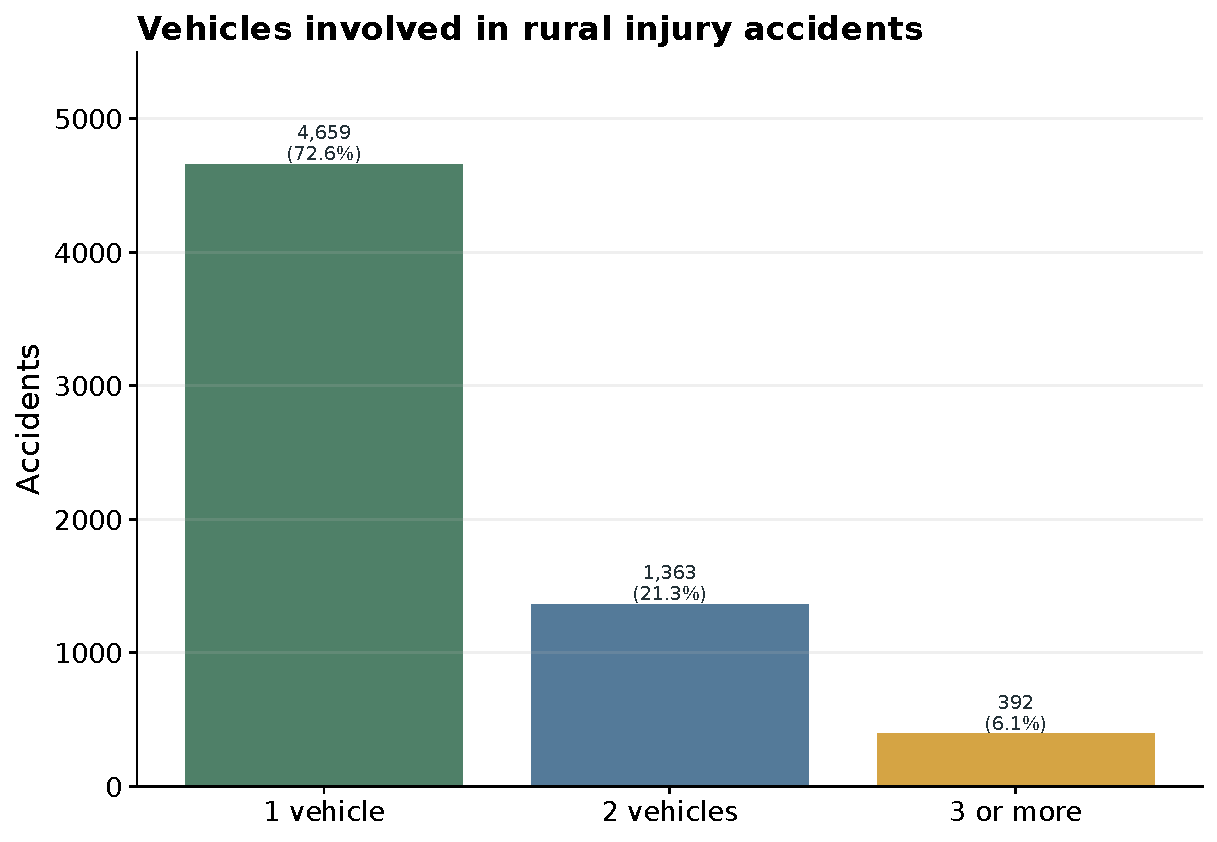
\includegraphics[width=0.72\textwidth]{vehicles_per_accident.pdf}
\caption[Registered vehicles involved in rural injury accidents.]{Number of registered vehicles involved in the 6,414 rural injury
accidents. Counts describe the selected sample, not risk by vehicle count.}
\label{fig:vehicles-per-accident}
\end{figure}

\begin{figure}[htbp]
\centering
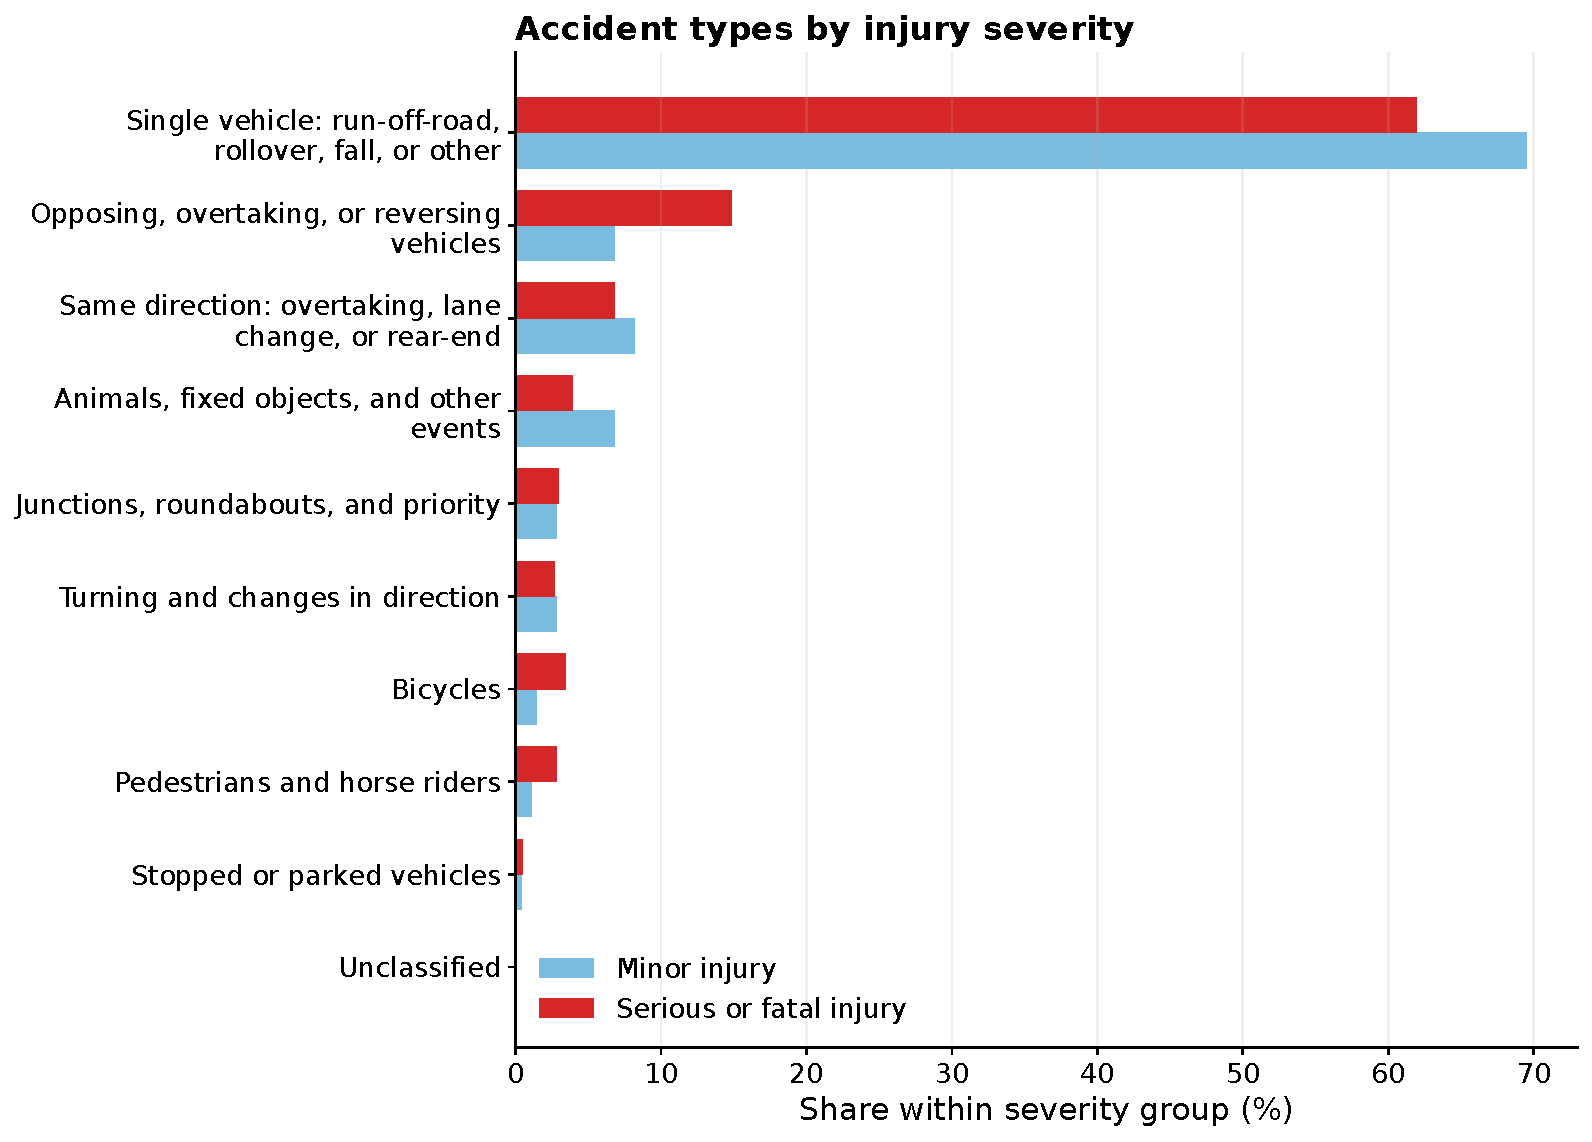
\includegraphics[width=\textwidth]{accident_types_by_severity.pdf}
\caption[Accident-type composition by injury severity.]{Accident-type composition for minor injury (blue, code 3) and
serious or fatal injury (red, codes 1--2). Percentages sum to 100 within
each separate severity group.}
\label{fig:accident-types-severity}
\end{figure}

\clearpage
\section{Supporting Statistical Models}
\label{app:statistical-models}

This section gives the fitting details for the supporting matched-time and severity models.

The matched-time models use \texttt{statsmodels} version 0.14.6 and
\texttt{ConditionalLogit}, maximising the conditional logistic likelihood by
BFGS optimisation. Conditioning on the single case in each stratum eliminates
its intercept. Model-based covariance is the inverse negative Hessian of the
conditional log-likelihood; ORs and normal-Wald intervals follow
Equation~\ref{eq:odds-ratio-ci}.

The joint model includes mean-wind and temperature categories together, using
these same references and matched times with both measures available. The
daylight model compares darkness and civil twilight with daylight at the
accident location, under the same calendar matching and fitting procedure.
The seasonal model uses mean-wind groups 0--10 (reference), 10--15, and at least
15 m/s, with Winter as the reference season for wind interactions. A
likelihood-ratio test compares models with and without the six interaction
terms against a chi-squared distribution with six degrees of freedom.
Season-specific log-odds contrasts combine the relevant coefficients; their
standard errors use the full covariance matrix, with intervals computed as in
Equation~\ref{eq:odds-ratio-ci} using 1.96.

The adjusted severity model uses \texttt{statsmodels.Logit}, estimating an
intercept and categorical coefficients jointly by Bernoulli maximum
likelihood with Newton optimisation. Among injury accidents with qualifying
wind, temperature, and daylight, the outcome is one for serious or fatal
injury (codes 1--2) and zero for minor injury (code 3). Reference categories
are mean wind 0--10 m/s, temperature 0--3\(^{\circ}\)C, daylight, 10:00--16:00,
and Summer. The fit requests HC1 heteroskedasticity-robust covariance;
adjusted ORs and normal-Wald intervals follow
Equation~\ref{eq:odds-ratio-ci} with those robust standard errors.
These ORs concern severity conditional on an injury accident, not accident
occurrence.

Table~\ref{tab:severity-conditions} shows the adjusted comparison of
serious or fatal and minor-injury accidents. It describes severity among
recorded injury accidents; it does not estimate accident occurrence or risk
per vehicle-kilometre.

\begin{table}[H]
\centering
\footnotesize
\caption{Adjusted odds ratios for a serious-or-fatal outcome among recorded injury accidents. All listed variables are included in the same model.}
\label{tab:severity-conditions}
\begin{tabularx}{\textwidth}{L{0.20\textwidth}L{0.45\textwidth}X}
\toprule
Variable & Comparison & Adjusted OR (95\% CI) \\
\midrule
Mean wind & 10-15 m/s vs 0-10 m/s & 0.99 (0.82--1.21) \\ \grayhline
Mean wind & $\geq$15 m/s vs 0-10 m/s & 0.93 (0.69--1.26) \\ \grayhline
Temperature & <-6 °C vs 0-3 °C & 1.13 (0.79--1.62) \\ \grayhline
Temperature & -6--3 °C vs 0-3 °C & 0.85 (0.63--1.15) \\ \grayhline
Temperature & -3-0 °C vs 0-3 °C & 0.83 (0.66--1.04) \\ \grayhline
Temperature & 3-6 °C vs 0-3 °C & 1.11 (0.88--1.39) \\ \grayhline
Temperature & 6-9 °C vs 0-3 °C & 1.41 (1.10--1.79) \\ \grayhline
Temperature & 9-12 °C vs 0-3 °C & 1.28 (0.98--1.68) \\ \grayhline
Temperature & 12-15 °C vs 0-3 °C & 1.33 (0.98--1.81) \\ \grayhline
Temperature & $\geq$15 °C vs 0-3 °C & 1.21 (0.83--1.76) \\ \grayhline
Daylight & Darkness vs Daylight & 0.89 (0.71--1.12) \\ \grayhline
Daylight & Civil twilight vs Daylight & 1.09 (0.87--1.36) \\ \grayhline
Time of day & 00-06 vs 10-16 & 0.86 (0.64--1.16) \\ \grayhline
Time of day & 06-10 vs 10-16 & 0.65 (0.52--0.82) \\ \grayhline
Time of day & 16-20 vs 10-16 & 0.98 (0.84--1.14) \\ \grayhline
Time of day & 20-24 vs 10-16 & 0.77 (0.61--0.98) \\ \grayhline
Season & Winter vs Summer & 0.82 (0.64--1.05) \\ \grayhline
Season & Spring vs Summer & 0.96 (0.78--1.18) \\ \grayhline
Season & Autumn vs Summer & 0.83 (0.65--1.05) \\
\bottomrule
\end{tabularx}
\end{table}


\clearpage
\section{Period and Counter-Era Sensitivity}
\label{app:period-sensitivity}

These checks assess whether period choice changes the upper-wind pattern.

Figures~\ref{fig:oe-early-period} and \ref{fig:oe-counter-period} repeat the
weather-frequency comparison for 2007--2018 and 2019--2024. They are supporting
All year checks; upper-bin counts should be read alongside the ratios.

\begin{figure}[!htbp]
\centering
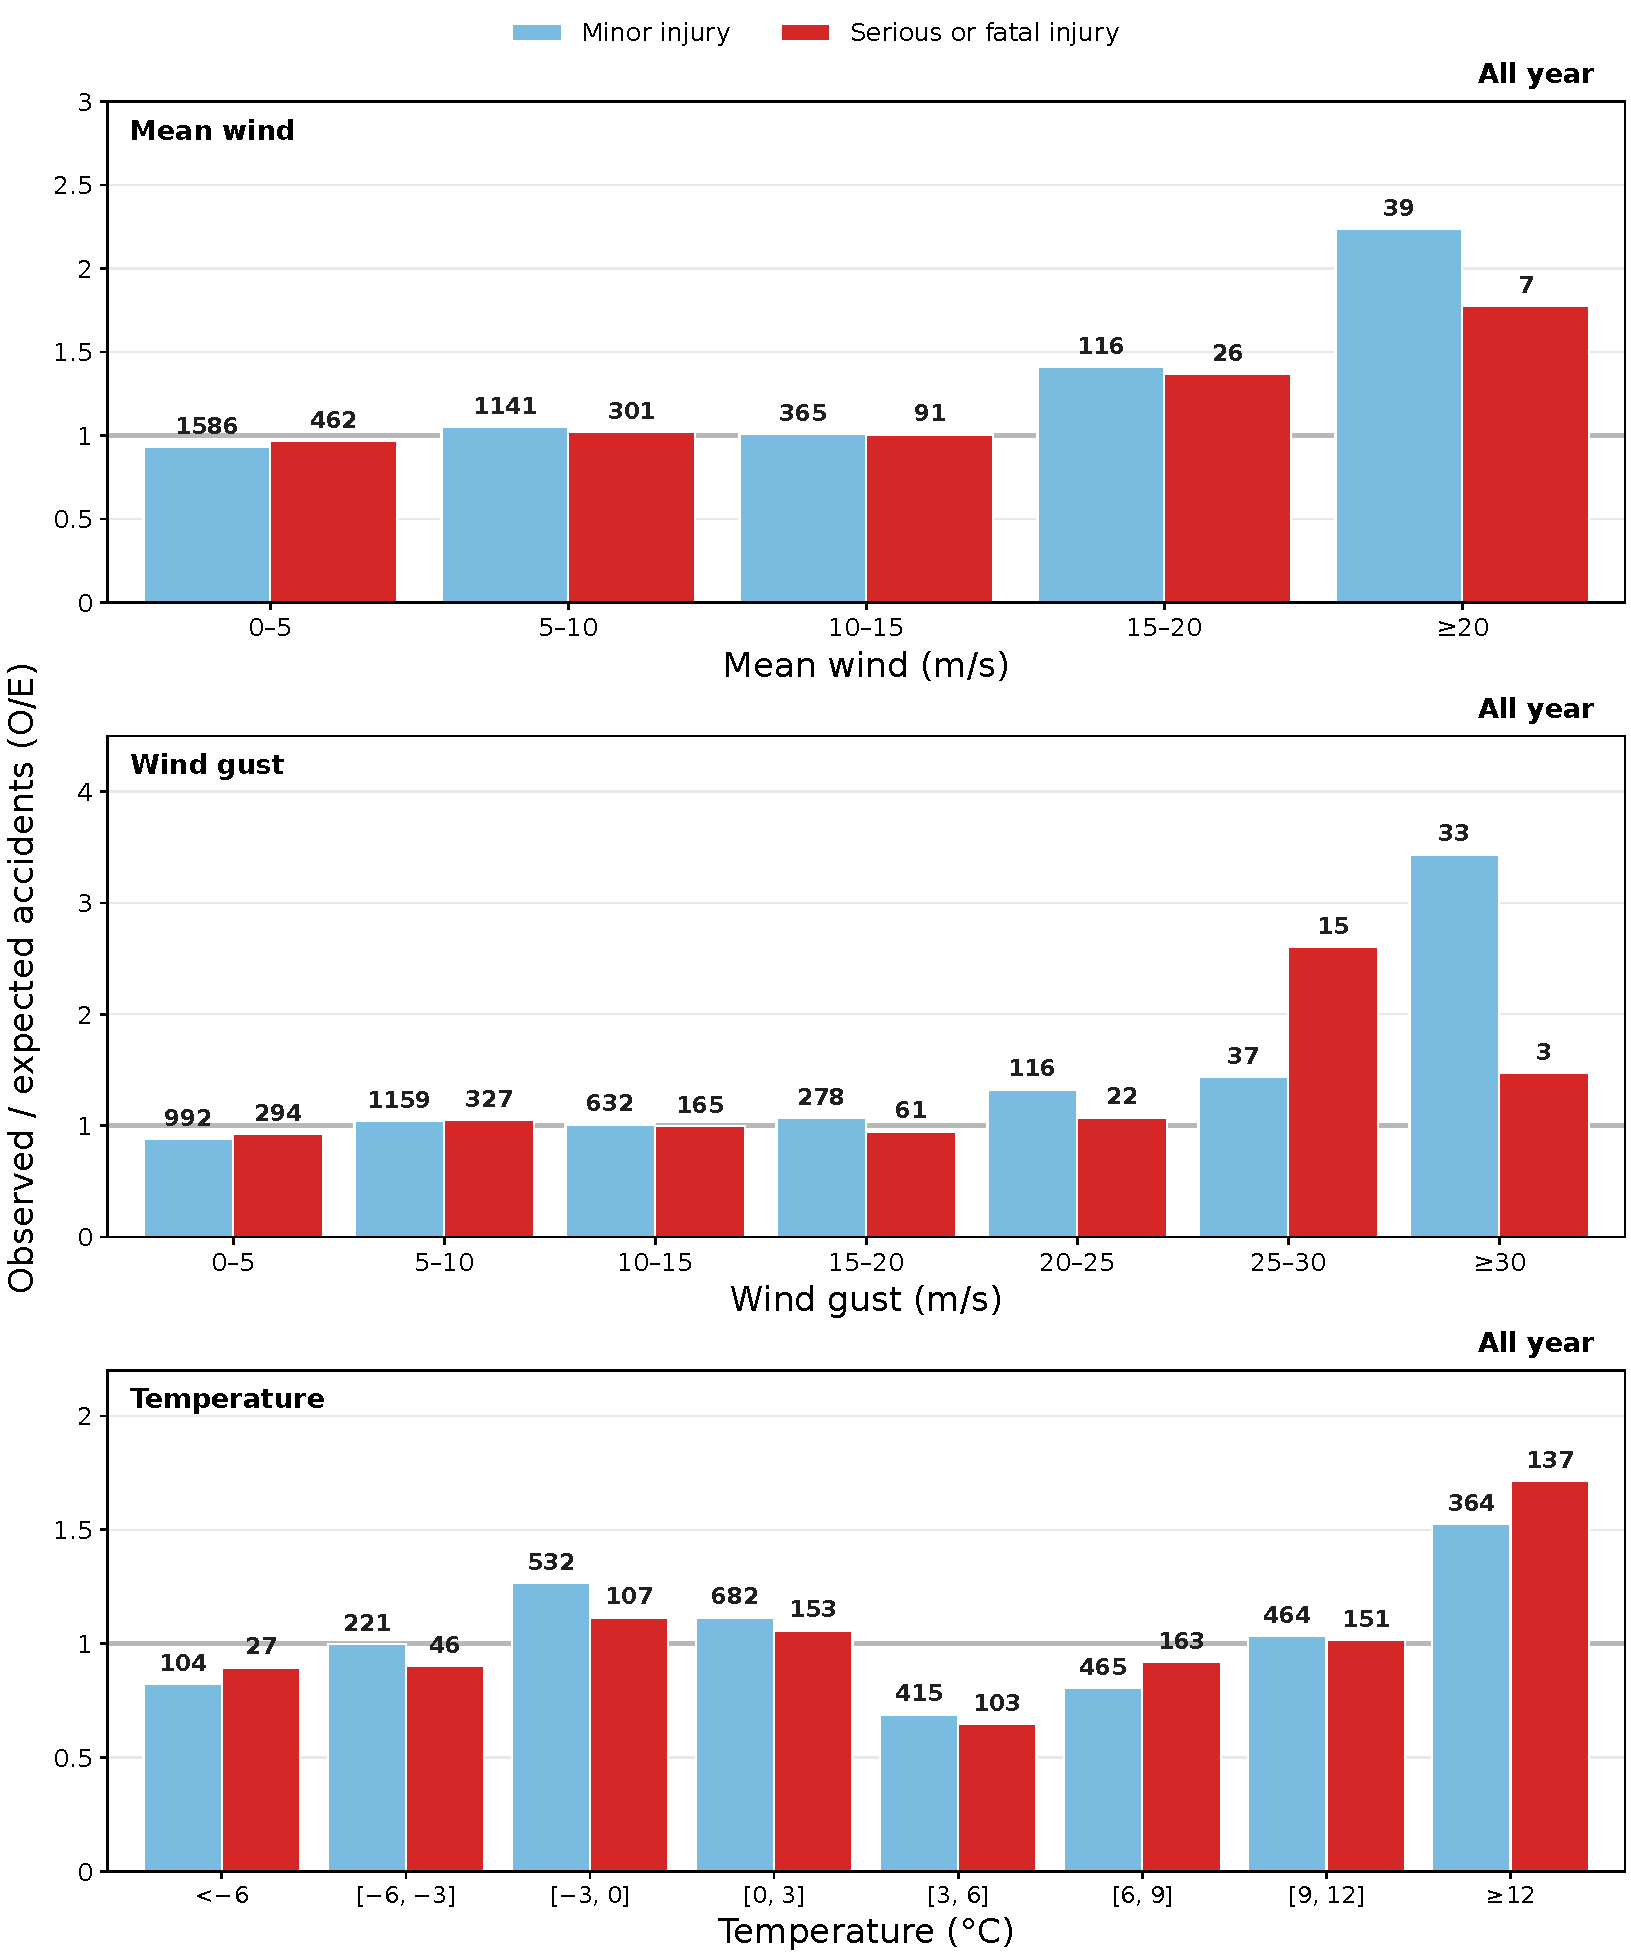
\includegraphics[width=\textwidth,height=0.65\textheight,keepaspectratio]{weather_oe_2007_2018.pdf}
\caption[All year weather-frequency O/E, 2007--2018.]{All year weather-frequency O/E for rural injury accidents, 2007--2018, with
accidents and background weather restricted to the same period. Blue and red
show minor and serious or fatal injury; labels give counts and the line marks
O/E = 1.}
\label{fig:oe-early-period}
\end{figure}

\begin{figure}[p]
\centering
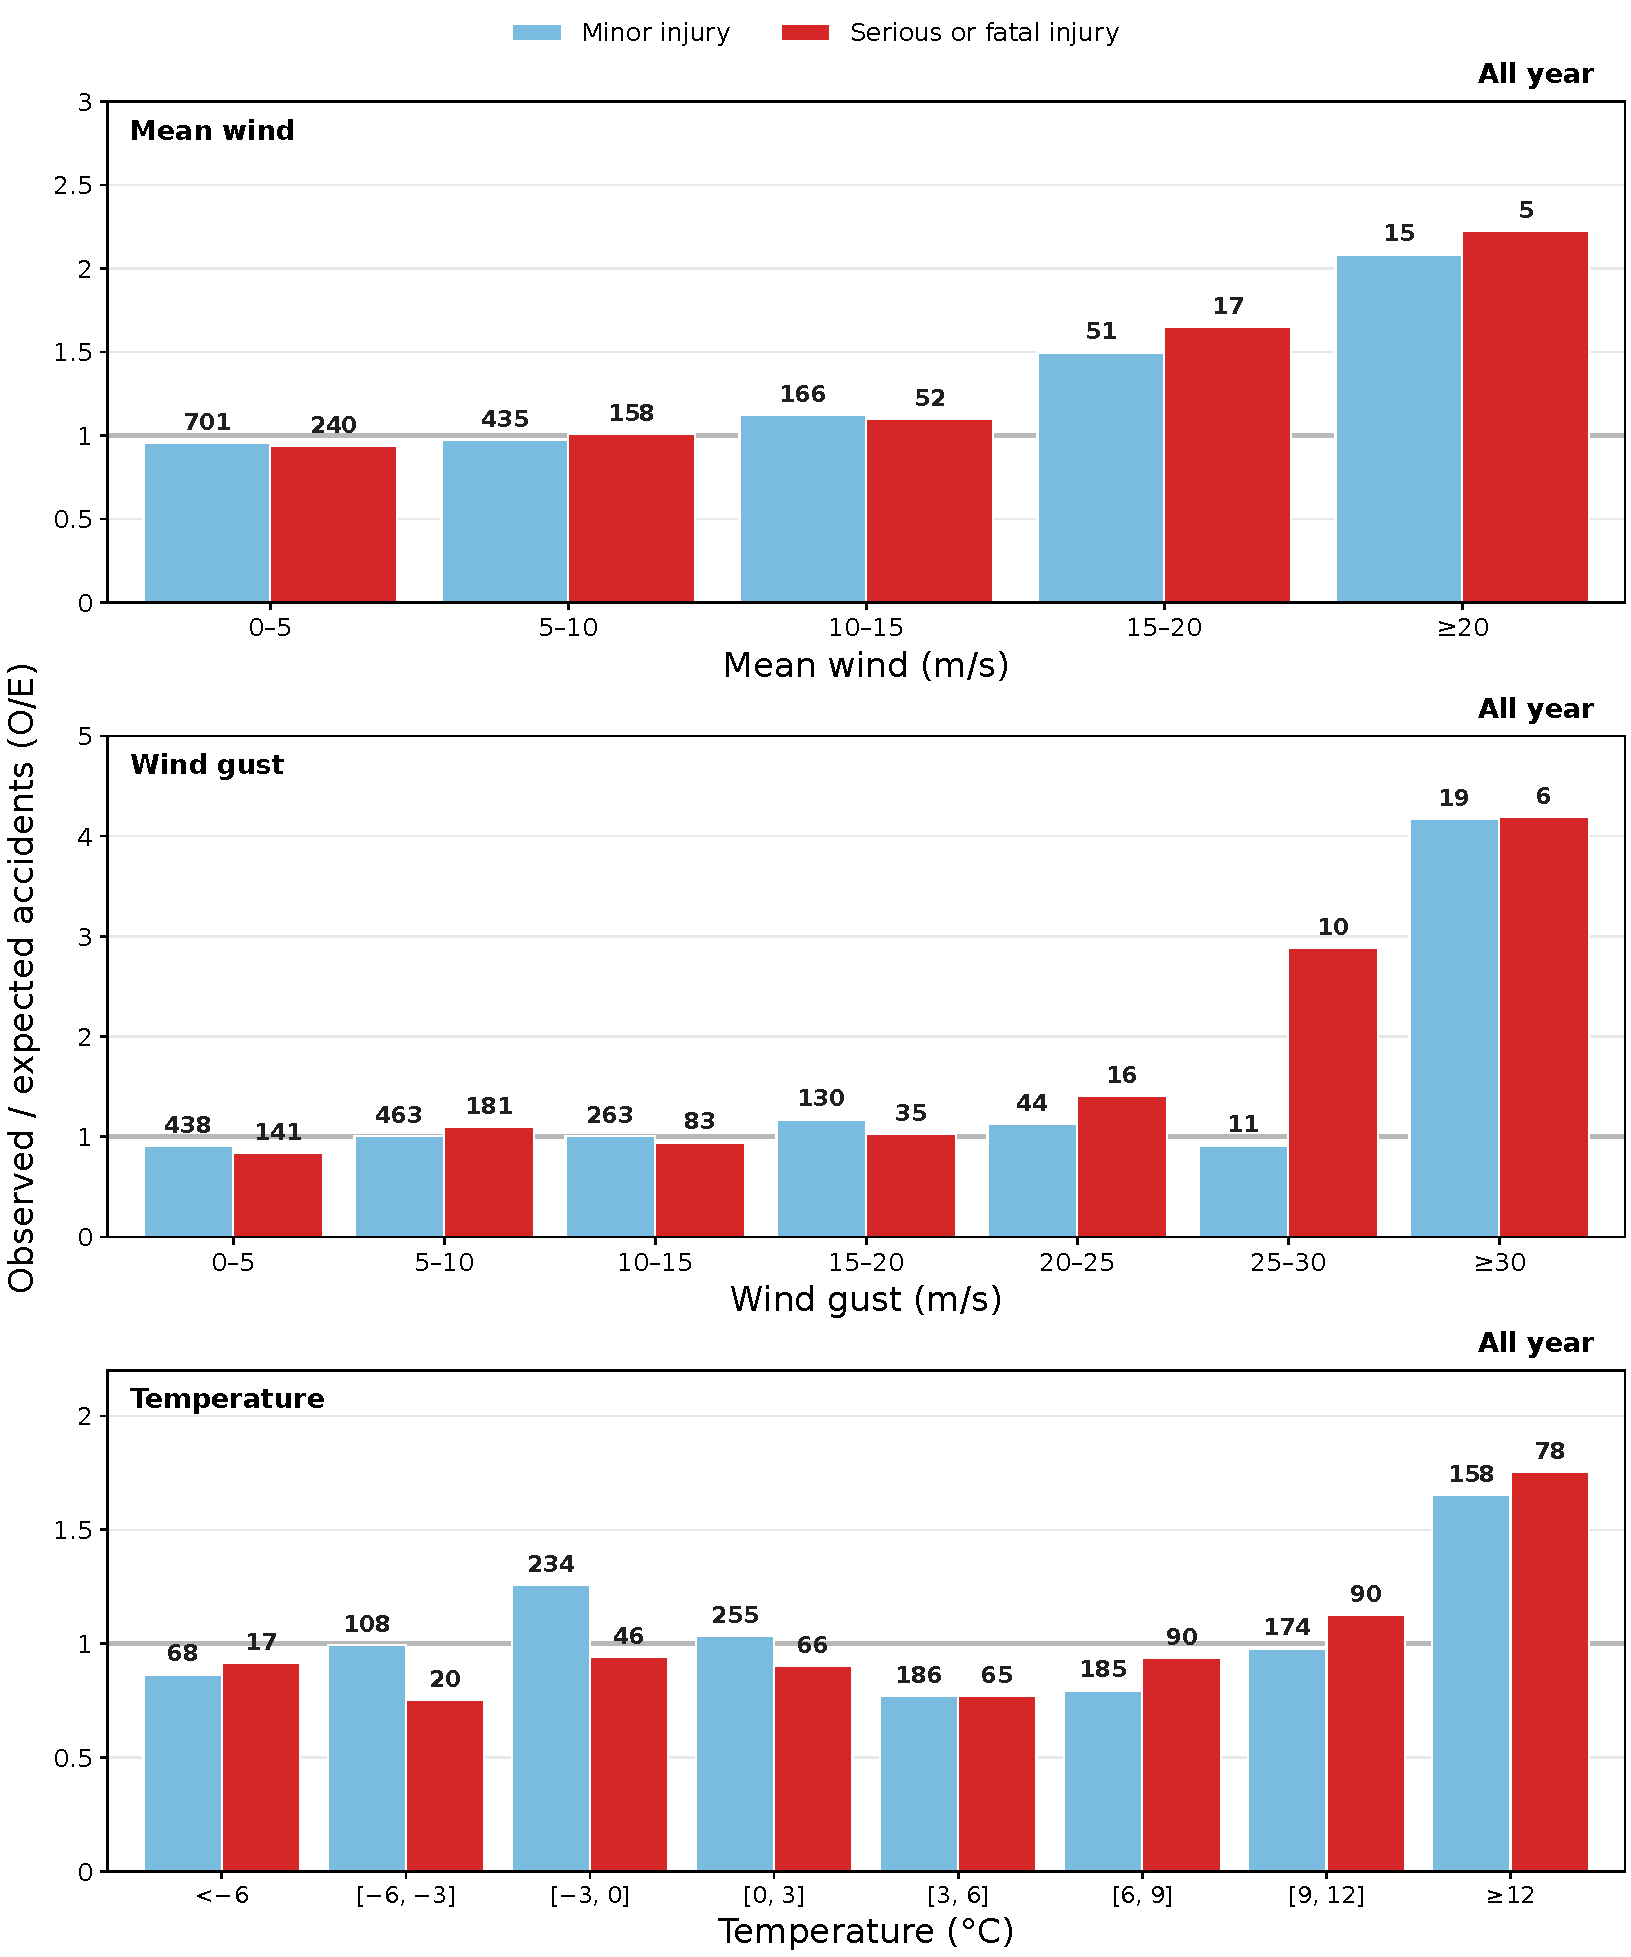
\includegraphics[width=\textwidth,height=0.73\textheight,keepaspectratio]{weather_oe_2019_2024.pdf}
\caption[All year weather-frequency O/E, 2019--2024.]{All year weather-frequency O/E for rural injury accidents, 2019--2024, with
accidents and background weather restricted to the same period. Blue and red
show minor and serious or fatal injury; labels give counts and the line marks
O/E = 1.}
\label{fig:oe-counter-period}
\end{figure}

Figure~\ref{fig:corrected-counter-period} applies the traffic correction within
2019--2024, allowing comparison with the uncorrected counter-era population in
Figure~\ref{fig:oe-counter-period}. Its temperature panel is corrected
weather-frequency O/E, not a VKT rate.

\begin{figure}[p]
\centering
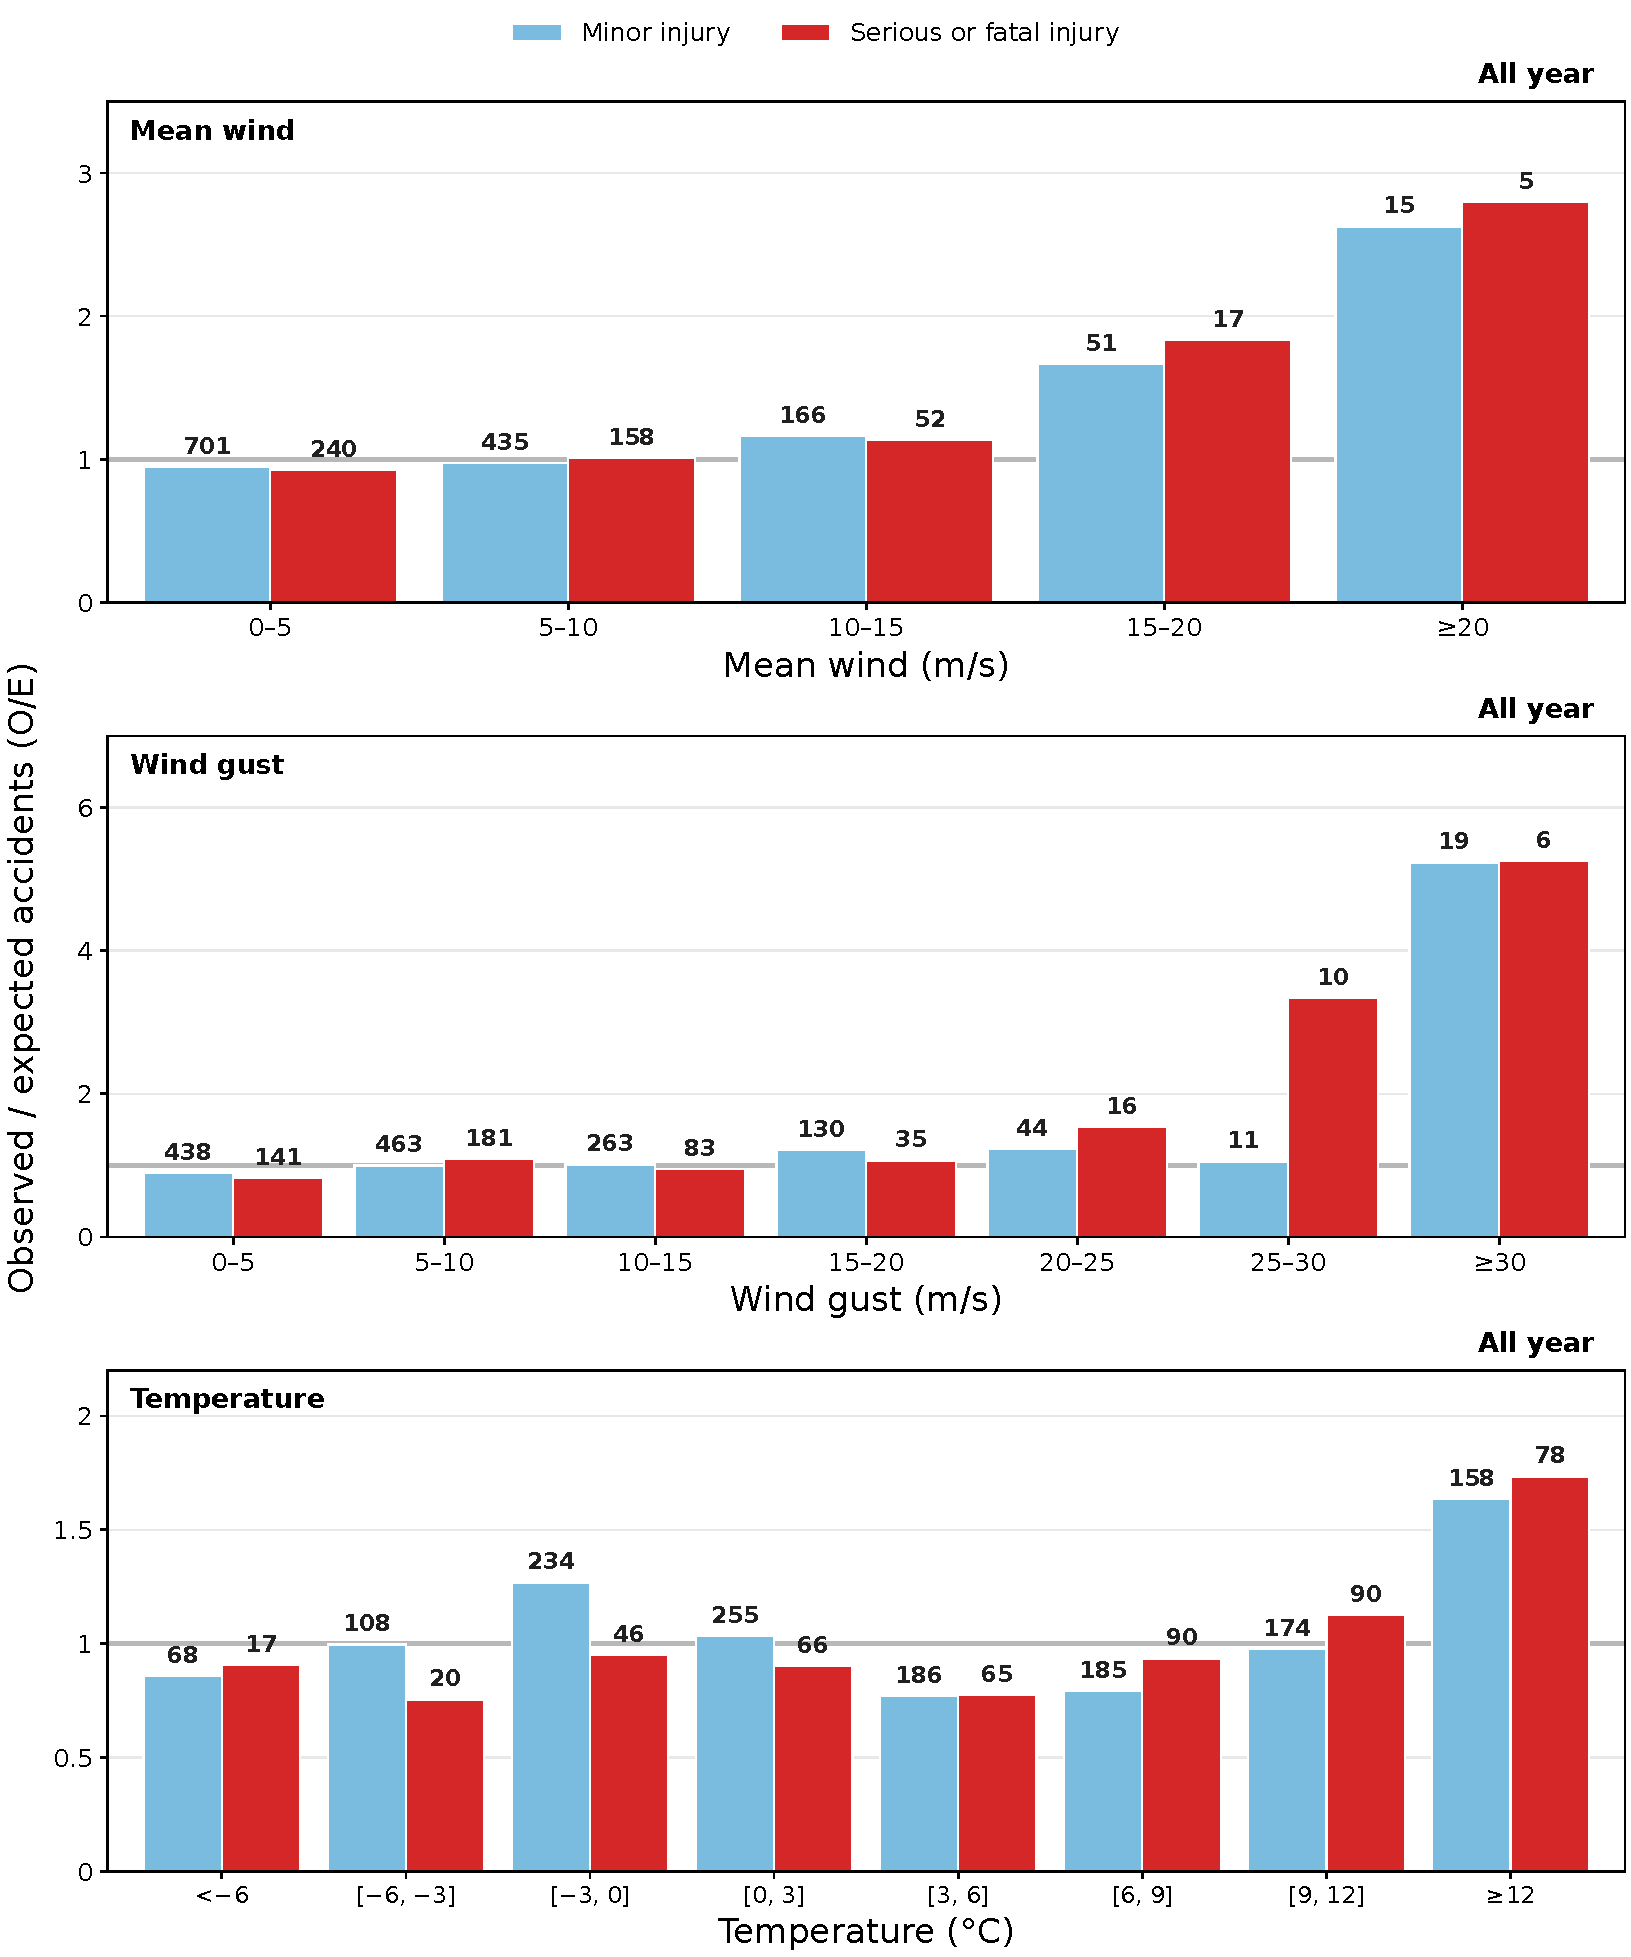
\includegraphics[width=\textwidth,height=0.73\textheight,keepaspectratio]{weather_oe_traffic_corrected_2019_2024.pdf}
\caption[Traffic-corrected All year O/E by injury group, 2019--2024.]{Approximately traffic-corrected O/E for rural injury accidents, 2019--2024,
All year. Blue and red show minor and serious or fatal injury using reweighted
expected counts; labels give observed accidents and the line marks O/E = 1.}
\label{fig:corrected-counter-period}
\end{figure}
\clearpage

\section{Supporting Allocated Daily-Counter Analysis}
\label{app:allocated-daily-counter}

This analysis checks the wind association under an alternative counter-linked
exposure construction. The supporting model uses observed 24-hour traffic
totals and allocates them across wind intervals according to each day's valid
10-minute weather observations. Directional channels are first summed to one
count for each physical counter and date. Accidents require a counter on the
exact registered road section and year, positive traffic on the accident date,
and a qualifying accident-time mean-wind observation. Eligible counter-days
require at least 108 valid 10-minute observations over the full day. The
allocated traffic is

\begin{equation}
\label{eq:allocated-counter-traffic}
\widehat Q_{cdj}=Q_{cd}\frac{N_{cdj}}{N_{cd}},
\end{equation}

where \(c\) indexes physical counters, \(d\) dates, and \(j\) wind intervals;
\(Q_{cd}\) is observed 24-hour traffic, \(N_{cdj}\) counts valid 10-minute
observations in interval \(j\), \(N_{cd}\) counts all valid observations that
day, and \(\widehat Q_{cdj}\) is traffic allocated to that interval.
Accidents use event-time mean wind from the denominator's station.
The allocation assumes uniform traffic across valid observation times.

Traffic and accidents are aggregated by counter, year, and wind interval.
The model uses \texttt{ConditionalPoisson} from \texttt{statsmodels} to estimate
coefficients for
10--15 and at least 15 m/s relative to 0--10 m/s. BFGS maximises the Poisson
likelihood conditional on each counter--year's total accident count, removing
its intercept. The offset is the logarithm of summed allocated traffic. An offset has its
coefficient fixed at one: it accounts for differing exposure so coefficients
compare accident rates rather than counts. Here exposure is allocated vehicle
counts, not vehicle-kilometres. Rate ratios are \(\exp(\widehat\beta)\), where
\(\widehat\beta\) is the fitted log-rate contrast. Normal-Wald 95\% intervals
use the same exponentiated-coefficient construction as
Equation~\ref{eq:odds-ratio-ci}, with standard errors from the inverse negative
Hessian of the conditional log-likelihood.

This supporting model is separate from the 694-accident main VKT analysis. The
tables below show how the 2019--2024 rural injury sample narrows under its
linkage. The 767 records at the last broad selection step include five records
that do not enter the final allocated-rate model, which retains 762 accidents.

Table~\ref{tab:allocated-selection} traces the linkage exclusions for this
supporting sample.

\begin{table}[H]
\centering
\small
\caption{Selection of accidents for the observed daily-counter analysis}

\begin{tabularx}{0.86\textwidth}{Xrr}
\toprule
Selection step & Accidents & Share of 2019--2024 sample \\
\midrule
Rural injury accidents in 2019--2024 & 1,863 & 100.0\% \\ \grayhline
Exact road-section/year counter candidate & 864 & 46.4\% \\ \grayhline
Assigned counter within 20 km & 863 & 46.3\% \\ \grayhline
Positive count and valid full-day wind & 767 & 41.2\% \\
\bottomrule
\end{tabularx}
\end{table}


Table~\ref{tab:allocated-sample} compares retained accidents with the broader
sample and excluded groups by severity, vehicles and season, making selection
differences visible.

\begin{table}[H]
\centering
\footnotesize
\caption{Characteristics of accidents retained and excluded by the daily-counter linkage}

\begin{tabularx}{\textwidth}{Xrrrr}
\toprule
Characteristic & All & No link & Linked, excluded & Retained \\
\midrule
Accidents & 1,863 & 999 & 106 & 758 \\ \grayhline
Share of all accidents & 100.0\% & 53.6\% & 5.7\% & 40.7\% \\ \grayhline
Distinct road sections & 563 & 374 & 59 & 189 \\ \grayhline
Serious or fatal & 25.6\% & 29.4\% & 17.9\% & 21.6\% \\ \grayhline
One vehicle & 67.7\% & 75.2\% & 54.7\% & 59.8\% \\ \grayhline
Winter & 32.6\% & 28.0\% & 41.5\% & 37.3\% \\ \grayhline
Spring & 13.0\% & 11.7\% & 8.5\% & 15.4\% \\ \grayhline
Summer & 36.0\% & 41.8\% & 33.0\% & 28.6\% \\ \grayhline
Autumn & 18.4\% & 18.4\% & 17.0\% & 18.6\% \\
\bottomrule
\end{tabularx}
\end{table}


The geographic selectivity of this traffic-linked sample is documented in
Figure~\ref{fig:counter-coverage}.

\begin{figure}[H]
\centering
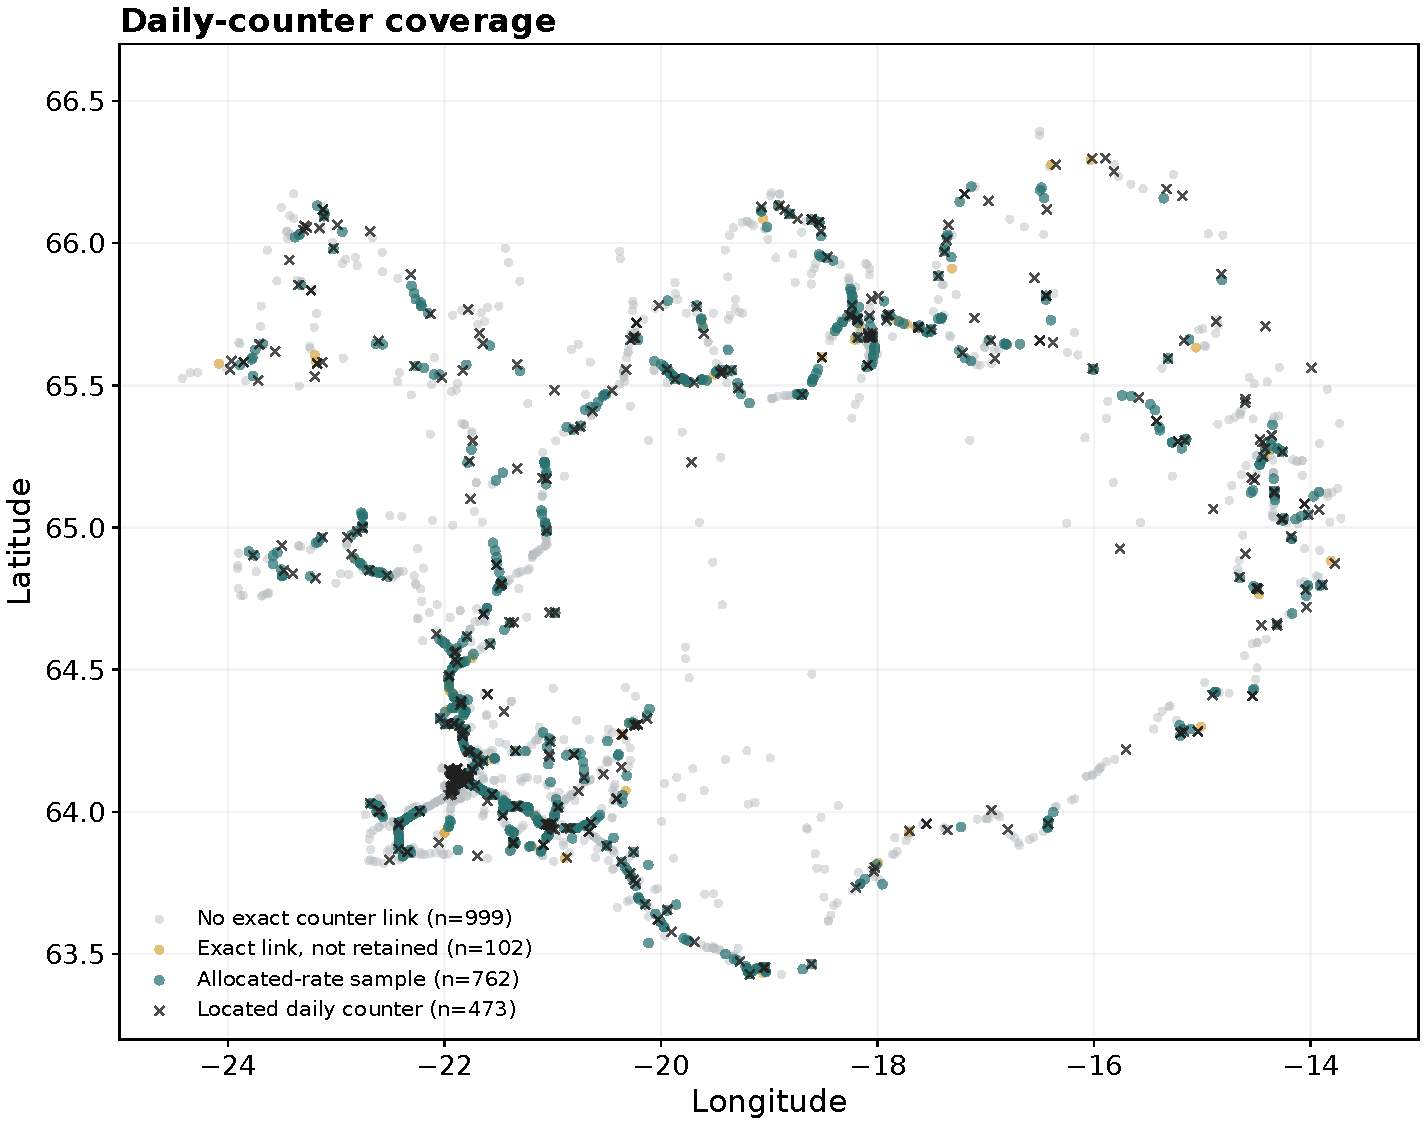
\includegraphics[width=0.9\textwidth]{counter_coverage.pdf}
\caption[Coverage of the supporting allocated daily-counter sample.]{Geographic coverage of located daily counters and rural injury
accidents retained or excluded by the daily-counter linkage, 2019--2024.}
\label{fig:counter-coverage}
\end{figure}

\section{Traffic Sensitivity Checks}
\label{app:traffic-sensitivity}

These checks assess sensitivity to counter assignment and recorded zero traffic.

Table~\ref{tab:allocated-radius} is a separate daily-mean-wind check under
5, 10, and 20 km accident-to-counter assignment limits. It classifies each
whole day's accident count and observed traffic by that day's mean wind,
without allocation among 10-minute weather intervals. The conditional Poisson
fit otherwise uses the counter--year strata, 0--10 m/s reference, BFGS
estimation, and RR/CI calculation described above; its offset is log summed
observed daily traffic in each counter--year--wind group. The upper bin is at
least 15 m/s. Included accidents count the linked sample before model filtering.

\begin{table}[H]
\centering
\small
\caption[Assignment-distance sensitivity of the daily-mean-wind model.]{Upper-bin estimate from the daily-mean-wind counter model under three accident-to-counter assignment distances.}
\label{tab:allocated-radius}

\begin{tabular}{rrrrr}
\toprule
Maximum distance & Included accidents & Upper-bin accidents & Rate ratio & 95\% CI \\
\midrule
5 km & 585 & 12 & 2.91 & 1.58--5.37 \\ \grayhline
10 km & 750 & 14 & 2.78 & 1.58--4.88 \\ \grayhline
20 km & 767 & 14 & 2.73 & 1.55--4.78 \\
\bottomrule
\end{tabular}
\end{table}


Table~\ref{tab:traffic-sensitivity} checks the effect of excluding recorded
zero counter-days from the daily traffic-response estimate. This supporting
check groups whole days by daytime mean wind (10:00--21:59) and compares
summed observed traffic with the counter--year--month--weekday mean expectation,
recomputed for each zero-count policy. Its 95\% intervals are the 2.5th and
97.5th percentiles of 1,000 bootstrap replicates that resample physical counters
with replacement, keeping their observed and expected traffic totals together.
The precomputed calendar expectations remain fixed within each bootstrap.

\begin{table}[H]
\centering
\footnotesize
\caption{Effect of excluding zero counter-days on the daily traffic response.}
\label{tab:traffic-sensitivity}
\begin{tabularx}{\textwidth}{L{0.19\textwidth}L{0.27\textwidth}L{0.22\textwidth}X}
\toprule
Check & Data included & Estimate (95\% interval) & Records \\
\midrule
Daily traffic, 20--25 m/s & Retain zero counter-days & 68.94\% (62.33--74.09) & 1,175 days \\ \grayhline
Daily traffic, 20--25 m/s & Exclude zero counter-days & 69.29\% (62.70--74.52) & 1,090 days \\
\bottomrule
\end{tabularx}
\end{table}



\end{document}
